\documentclass[11pt]{article}
\usepackage[margin=24mm]{geometry}\usepackage[T1]{fontenc}
\usepackage{amsmath,amssymb,amsthm,mathtools,mathrsfs,longtable,booktabs,array,graphicx,xurl}
\usepackage[hidelinks,hypertexnames=false]{hyperref}
\allowdisplaybreaks\setlength{\emergencystretch}{3em}
\providecommand{\tightlist}{\setlength{\itemsep}{0pt}\setlength{\parskip}{0pt}}
\DeclareUnicodeCharacter{03C0}{\ensuremath{\pi}}
\DeclareUnicodeCharacter{03C7}{\ensuremath{\chi}}
\DeclareUnicodeCharacter{03A6}{\ensuremath{\Phi}}
\DeclareUnicodeCharacter{0394}{\ensuremath{\Delta}}
\DeclareUnicodeCharacter{0393}{\ensuremath{\Gamma}}
\DeclareUnicodeCharacter{039B}{\ensuremath{\Lambda}}
\DeclareUnicodeCharacter{03C3}{\ensuremath{\sigma}}
\DeclareUnicodeCharacter{03B7}{\ensuremath{\eta}}
\DeclareUnicodeCharacter{03C4}{\ensuremath{\tau}}
\DeclareUnicodeCharacter{03B4}{\ensuremath{\delta}}
\DeclareUnicodeCharacter{03B3}{\ensuremath{\gamma}}
\DeclareUnicodeCharacter{03B1}{\ensuremath{\alpha}}
\DeclareUnicodeCharacter{03B2}{\ensuremath{\beta}}
\DeclareUnicodeCharacter{03C1}{\ensuremath{\rho}}
\DeclareUnicodeCharacter{03BA}{\ensuremath{\kappa}}
\DeclareUnicodeCharacter{03BB}{\ensuremath{\lambda}}
\DeclareUnicodeCharacter{03B8}{\ensuremath{\theta}}
\DeclareUnicodeCharacter{03B5}{\ensuremath{\varepsilon}}
\DeclareUnicodeCharacter{2208}{\ensuremath{\in}}
\DeclareUnicodeCharacter{2264}{\ensuremath{\le}}
\DeclareUnicodeCharacter{2265}{\ensuremath{\ge}}
\DeclareUnicodeCharacter{2260}{\ensuremath{\ne}}
\DeclareUnicodeCharacter{2192}{\ensuremath{\to}}
\DeclareUnicodeCharacter{2282}{\ensuremath{\subset}}
\DeclareUnicodeCharacter{2286}{\ensuremath{\subseteq}}
\DeclareUnicodeCharacter{2297}{\ensuremath{\otimes}}
\DeclareUnicodeCharacter{03A3}{\ensuremath{\Sigma}}
\DeclareUnicodeCharacter{221A}{\ensuremath{\surd}}
\DeclareUnicodeCharacter{221E}{\ensuremath{\infty}}
\DeclareUnicodeCharacter{00B2}{\ensuremath{{}^2}}
\DeclareUnicodeCharacter{00B3}{\ensuremath{{}^3}}
\DeclareUnicodeCharacter{2074}{\ensuremath{{}^4}}
\DeclareUnicodeCharacter{2080}{\ensuremath{{}_0}}
\DeclareUnicodeCharacter{2081}{\ensuremath{{}_1}}
\DeclareUnicodeCharacter{2082}{\ensuremath{{}_2}}
\DeclareUnicodeCharacter{2096}{\ensuremath{{}_k}}
\DeclareUnicodeCharacter{2212}{\ensuremath{-}}
\DeclareUnicodeCharacter{00D7}{\ensuremath{\times}}
\DeclareUnicodeCharacter{00B1}{\ensuremath{\pm}}
\DeclareUnicodeCharacter{2202}{\ensuremath{\partial}}
\DeclareUnicodeCharacter{2225}{\ensuremath{\Vert}}
\DeclareUnicodeCharacter{2113}{\ensuremath{\ell}}
\DeclareUnicodeCharacter{211D}{\ensuremath{\mathbb R}}
\DeclareUnicodeCharacter{2102}{\ensuremath{\mathbb C}}
\DeclareUnicodeCharacter{03BC}{\ensuremath{\mu}}
\DeclareUnicodeCharacter{03B6}{\ensuremath{\zeta}}
\DeclareUnicodeCharacter{03BE}{\ensuremath{\xi}}
\DeclareUnicodeCharacter{220F}{\ensuremath{\prod}}
\begin{document}

\title{Split-Zero cohomology: exact degree changes in the original kernel metric}
\author{}\date{21 September 2026}\maketitle
The programme represents finite zero-divisor classes of the completed Riemann
zeta function by polynomials in an arithmetic theta-source Hilbert space.
The observation kernel receives its metric by minimizing over every original
source representative. The preceding edition expressed its determinant by
complete mixed relations. This edition calculates its exact change with degree.

CD1--22 gives every Gamma covariance entry, including reflected-node collisions,
and its full correction after compression. CD-C1--16 supplies the independent
coefficient, divided-jet and metric calculation. DS1--28 gives the exact
degree-step factors and the product for the original four cutoffs. The paired
quartet relation proves a strictly positive finite kernel return; its magnitude
at the unresolved large-degree $kq$ scale is not evaluated. No RH conclusion
or arithmetic-zero identification is claimed.

The complete seven-body predecessor follows the new proofs, with all its
human citations and original-source providers retained. Classical methods are
credited at their point of use. The source archive also contains three full
cumulative LaTeX successors; those large cumulative documents have not been
freshly compiled in this edition.

% BEGIN COMPLETE CD AND DEGREE STEP 20260921

\clearpage\begingroup
\part*{Every boundary-kernel entry and its exact compressed correction}
\newcommand{\cdrootC}{\mathbb C}
\newcommand{\cdrootR}{\mathbb R}
\newcommand{\cdrootconj}[1]{\overline{#1}}


\section{Source, mass, coordinates and scope}

This is a finite calculation on the original Gamma receiver MR22--23
\cite{cdroot:MR}%
% BEGIN VERIFIED PUBLIC PROOF LINK
~\href{https://github.com/KokunoYumeto/zeta-function-research-reader/blob/5992ad50c0f2a06921f1fcaded7b4e38097c0739/workbenches/splitzero-tandem/continuations/20260920-original-kernel-mixed-determinants/ORIGINAL_KERNEL_MIXED_DETERMINANT.tex\#L36}{[proof MR1]}%
% END VERIFIED PUBLIC PROOF LINK
{}, not a replacement of the arithmetic source or its original
coefficient frame. The underlying Christoffel--Darboux identity is
classical; Akemann--Vernizzi's original author source explicitly gives
its real-line formula and its algebraic continuation in the footnote
at \texttt{CD} \cite{cdroot:AV}. The exact Gamma recurrence and norms below
are the Meixner--Pollaczek formulas \cite{cdroot:DLMF}, transported in the
original JM26 and KG6 coordinates \cite{cdroot:JM,cdroot:KG}%
% BEGIN VERIFIED PUBLIC PROOF LINK
~\href{https://github.com/KokunoYumeto/zeta-function-research-reader/blob/5992ad50c0f2a06921f1fcaded7b4e38097c0739/workbenches/splitzero-tandem/continuations/20260920-original-kernel-mixed-determinants/providers/JOINT_MINIMUM_RECEIVERS.tex\#L286}{[proof JM21]} \href{https://github.com/KokunoYumeto/zeta-function-research-reader/blob/5992ad50c0f2a06921f1fcaded7b4e38097c0739/workbenches/splitzero-tandem/continuations/20260920-original-kernel-mixed-determinants/providers/KERNEL_GAMMA_INDEPENDENT.tex\#L73}{[proof KG1]}%
% END VERIFIED PUBLIC PROOF LINK
{}. We derive every finite
identity used here. No large-degree coefficient, limit estimate,
arithmetic zero statement, or priority claim about the classical
identity is asserted.

The retained density, original physical coordinate and its complex
evaluation chart are
\begin{equation}\label{cdroot:eq:source}
 d\sigma(y)=\frac{|\Gamma(1/4+iy/2)|^2}{2\pi}\,dy,
 \quad M_\sigma=\sqrt{2\pi},\quad c=k/2,
 \quad S=c+iy,
 \quad u=\frac{v-c}{i},\quad w=\frac{z-c}{i}.
 \tag{CD1}
\end{equation}
In formulas with two scalar polynomial variables, write \(x=u\) and
\(t=\overline w\); these variables are independent during
differentiation. An asterisk on a matrix always means conjugate
transpose. The source inner product is
\(\langle P,Q\rangle=\int\overline{P(c+iy)}Q(c+iy)\,d\sigma(y)\).

Here is the mass check, retaining the scale in \(y\). The original DLMF
weight and norm at \(\lambda=1/4,\phi=\pi/2\) are
\[
 |\Gamma(1/4+ix)|^2\,dx,
 \qquad
 h_j=\frac{2\pi\Gamma(j+1/2)}{\sqrt2\,j!}.
\]
Set \(y=2x\) and
\(p_j(y)=j!P_j^{(1/4)}(y/2;\pi/2)\).
The measure becomes \(|\Gamma(1/4+ix)|^2dx/\pi\). Hence the actual
squared norm is
\begin{equation}\label{cdroot:eq:norm}
 \gamma_j=\frac{(j!)^2}{\pi}h_j
 =\sqrt2\,j!\Gamma(j+1/2)
 =\sqrt{2\pi}\,j!(1/2)_j.
 \tag{CD2}
\end{equation}
In particular \(\gamma_0=M_\sigma=\sqrt{2\pi}\). The exact density
change \(dy=2dx\) is already included in CD2.

The original generating function, after the same substitution, is
\[
 \sum_{j\geq0}\frac{p_j(y)}{j!}\zeta^j
 =(1+\zeta^2)^{-1/4}e^{y\arctan\zeta}.
\]
Its highest \(y\) coefficient proves monicity. Differentiating in
\(\zeta\) gives
\((1+\zeta^2)\partial_\zeta F=(y-\zeta/2)F\).
Coefficient comparison therefore proves the original recurrence
\begin{equation}\label{cdroot:eq:recurrence}
 p_0=1,\quad p_1=y,\quad
 p_{j+1}(y)=yp_j(y)-a_jp_{j-1}(y),
 \quad a_j=j(j-\tfrac12)=\frac{\gamma_j}{\gamma_{j-1}}
 \quad(j\geq1).
 \tag{CD3}
\end{equation}
All coefficients of \(p_j\) are real. We put \(p_{-1}=0\) only in
recurrences whose coefficient is zero; no negative-index norm is used.

\section{The two-polynomial identity and its sign}

For \(d\geq0\), set
\[
 \mathcal K_d(x,t)=\sum_{j=0}^{d-1}\frac{p_j(x)p_j(t)}{\gamma_j},
 \qquad K_d(v,\overline z)=\mathcal K_d(u,\overline w).
\]
An empty sum is zero. For \(d\geq1\), define
\[
 F_d(x,t)=p_d(x)p_{d-1}(t)-p_{d-1}(x)p_d(t).
\]
Then the exact polynomial identity is
\begin{equation}\label{cdroot:eq:cd}
 (x-t)\mathcal K_d(x,t)=\frac{F_d(x,t)}{\gamma_{d-1}}.
 \tag{CD4}
\end{equation}
To prove it without dividing by \(x-t\), put
\(T_j=p_{j+1}(x)p_j(t)-p_j(x)p_{j+1}(t)\).
The recurrence gives
\[
 (x-t)p_j(x)p_j(t)=T_j-a_jT_{j-1}.
\]
For \(j=0\) the second term is zero. Division by \(\gamma_j\) and
\(a_j/\gamma_j=1/\gamma_{j-1}\) make the finite sum telescope to
\(T_{d-1}/\gamma_{d-1}=F_d/\gamma_{d-1}\).
This proves \eqref{cdroot:eq:cd} as an identity in \(\cdrootC[x,t]\), including
\(x=t\). Away from that diagonal it gives
\begin{equation}\label{cdroot:eq:offdiagonal}
 \boxed{\mathcal K_d(x,t)=
 \frac{p_d(x)p_{d-1}(t)-p_{d-1}(x)p_d(t)}
      {\gamma_{d-1}(x-t)}.}
 \tag{CD5}
\end{equation}
At the diagonal, differentiation of the polynomial identity in \(x\)
and then setting \(x=t\) gives
\begin{equation}\label{cdroot:eq:diagonal}
 \boxed{\mathcal K_d(t,t)=
 \frac{p_d'(t)p_{d-1}(t)-p_{d-1}'(t)p_d(t)}{\gamma_{d-1}}.}
 \tag{CD6}
\end{equation}
At \(d=1\) both formulas give \(1/M_\sigma\), fixing the denominator
sign. At \(d=0\), the kernel and all its derivatives are zero; neither
CD5 nor CD6 is used.

The collision in these formulas is \(u=\overline w\), not merely
\(u=w\). For complex off-line arguments, the Hermitian kernel entry
\(\mathcal K_d(u,\overline u)\) usually belongs to CD5, not CD6.
CD6 applies when the two polynomial arguments coincide, whether or not
that common argument is real. Positivity is asserted for Hermitian Gram
matrices, not for every analytically continued scalar entry.

\section{Every divided jet, both away from and at a collision}

For a polynomial \(f\), write \(f^{[a]}=f^{(a)}/a!\). Define
\[
 F_{d;a,b}(x,t)=p_d^{[a]}(x)p_{d-1}^{[b]}(t)
             -p_{d-1}^{[a]}(x)p_d^{[b]}(t),
 \qquad
 \mathcal K_{d;r,s}=\frac{\partial_x^r\partial_t^s\mathcal K_d}{r!s!}.
\]
For all nonnegative integers \(r,s\), at \(x\ne t\),
\begin{equation}\label{cdroot:eq:jets-away}
 \boxed{\mathcal K_{d;r,s}(x,t)=\frac1{\gamma_{d-1}}
  \sum_{a=0}^r\sum_{b=0}^s
  \frac{(-1)^a\binom{a+b}{a}\,
        F_{d;r-a,s-b}(x,t)}{(x-t)^{a+b+1}}.}
 \tag{CD7}
\end{equation}
Indeed the divided \((a,b)\) derivative of \((x-t)^{-1}\) is
\((-1)^a\binom{a+b}{a}(x-t)^{-a-b-1}\). The divided-derivative product
rule is convolution with no further binomial factor. Applying it to
CD5 proves CD7.

At a collision \((x,t)=(\tau,\tau)\), the exact formula is
\begin{equation}\label{cdroot:eq:jets-collision}
 \boxed{\mathcal K_{d;r,s}(\tau,\tau)
  =\frac1{\gamma_{d-1}}
      \sum_{j=0}^{s}F_{d;r+1+j,s-j}(\tau,\tau)
  =-\frac1{\gamma_{d-1}}
      \sum_{j=0}^{r}F_{d;r-j,s+1+j}(\tau,\tau).}
 \tag{CD8}
\end{equation}
For a complete proof, expand both sides of
\(F_d(x,t)=\gamma_{d-1}(x-t)\mathcal K_d(x,t)\) at
\(x=\tau+h,t=\tau+z\). Equality of the coefficient of \(h^az^b\)
gives
\[
 F_{d;a,b}(\tau,\tau)=\gamma_{d-1}
 \bigl(\mathcal K_{d;a-1,b}(\tau,\tau)
       -\mathcal K_{d;a,b-1}(\tau,\tau)\bigr),
\]
where any negative derivative index means zero. Starting with
\((a,b)=(r+1,s)\) and iterating downward in \(s\) proves the first
sum. Starting with \((r,s+1)\) and iterating downward in \(r\)
proves the second. The expansion is finite, so there is no interchange
of infinite limiting operations. CD7--8 include arbitrary repeated
roots and all mixed divided jets. Derivatives beyond the degree are
zero, exactly as in the original finite kernel.

\section{The original \(S\) coordinate and its reflection denominator}

The monic polynomials in the physical coordinate are
\[
 P_j(v)=i^jp_j((v-c)/i),\qquad \|P_j\|^2=\gamma_j.
\]
The paired phases cancel in each kernel summand, so this is the same
\(K_d\) already defined. Since
\[
 u-\overline w=-i(v+\overline z-2c),
\]
and
\[
 F_d(u,\overline w)=-i\bigl(
 P_d(v)\overline{P_{d-1}(z)}+
 P_{d-1}(v)\overline{P_d(z)}\bigr),
\]
CD5 becomes
\begin{equation}\label{cdroot:eq:S-CD}
 \boxed{K_d(v,\overline z)=
 \frac{P_d(v)\overline{P_{d-1}(z)}+
       P_{d-1}(v)\overline{P_d(z)}}
      {\gamma_{d-1}(v+\overline z-2c)}.}
 \tag{CD9}
\end{equation}
This expression is used away from \(v+\overline z=2c\); the
polynomial extension supplies the remaining values. The numerator is a
sum and the denominator is a reflection sum. Replacing either by the
usual real-line difference would change the original coordinate.

The exact divided-jet transport is
\begin{equation}\label{cdroot:eq:S-jets}
 \frac{\partial_v^r\partial_{\overline z}^sK_d(v,\overline z)}{r!s!}
   =i^{-r}i^s\mathcal K_{d;r,s}(u,\overline w).
 \tag{CD10}
\end{equation}
This follows from \(\partial_v=i^{-1}\partial_u\) and
\(\partial_{\overline z}=i\partial_{\overline w}\), so it also
fixes the phases at collisions. For a direct formula in physical
variables, write \(G_d(v,b)=P_d(v)\overline{P_{d-1}(\overline b)}+
P_{d-1}(v)\overline{P_d(\overline b)}\), a polynomial in independent
variables \(v,b\), and use divided derivatives \(G_{d;a,b}\), with
the second subscript here an integer. Away from \(v+b=2c\), the
counterpart of CD7 has denominator \((v+b-2c)^{a+b+1}\) and sign
\((-1)^{a+b}\) in each summand. At a point \(v_0+b_0=2c\), it is
\begin{equation}\label{cdroot:eq:S-jets-collision}
 \frac{\partial_v^r\partial_b^sK_d(v,b)}{r!s!}
 \bigg|_{(v_0,b_0)}
  =\frac1{\gamma_{d-1}}
      \sum_{j=0}^s(-1)^jG_{d;r+1+j,s-j}(v_0,b_0).
 \tag{CD11}
\end{equation}
To prove this independently, expand
\(G_d=\gamma_{d-1}(v+b-2c)K_d\) at that point; the local linear
factor is now \(h+z\), so solving the same coefficient recurrence
alternates the signs. This agrees with CD10.

\section{Every entry at the original quartet and all four cutoffs}

The original simple-packet domain is
\[
 0<\delta<\tfrac12,\quad \gamma>2,\quad k\equiv1\pmod4,
 \quad k\geq9,\quad q=(k+1)^2,
\]
on the original five-orbit period locus of OCF \cite{cdroot:OCF}%
% BEGIN VERIFIED PUBLIC PROOF LINK
~\href{https://github.com/KokunoYumeto/zeta-function-research-reader/blob/5992ad50c0f2a06921f1fcaded7b4e38097c0739/workbenches/splitzero-tandem/continuations/20260920-original-kernel-mixed-determinants/providers/ORIGINAL_CONDUCTOR_STRIP_FRAME.tex\#L27}{[proof OCF1]}%
% END VERIFIED PUBLIC PROOF LINK
{}. Here
\(\gamma\) is the retained zero height, whereas \(\gamma_j\) is a
squared polynomial norm. The ordered roots and their exact charts are
\begin{equation}\label{cdroot:eq:roots}
 v_{ab}=c+(2a-k)\delta+i(2b-k)\gamma,
 \qquad u_{ab}=(2b-k)\gamma-i(2a-k)\delta,
 \quad 0\leq a,b\leq k.
 \tag{CD12}
\end{equation}
Distinctness follows by comparing the two real coordinates, since
\(\delta,\gamma>0\). However
\[
 u_{ab}=\overline{u_{a'b'}}
 \quad\Longleftrightarrow\quad b=b',\quad a'=k-a.
\]
Indeed equality of real parts gives \(b=b'\), and equality of imaginary
parts gives \(-(2a-k)=2a'-k\). Thus the full covariance has exactly
one collision entry per row, at its reflected column \((k-a,b)\).
There are \(q\) such ordered entries. Since \(k\) is odd, there are no
fixed points \(a=k-a\), and these are not its Hermitian diagonal
entries. Their CD6 values must be retained.

For \(d=N+1\), let \(C_d\) denote the matrix
\([\mathcal K_d(u_\alpha,\overline{u_\beta})]\) in exactly that
lexicographic root order. For every pair of entries it is computed from
the same two polynomials by
\begin{equation}\label{cdroot:eq:entry-recipe}
 (C_d)_{\alpha\beta}=
 \begin{cases}
 \dfrac{p_d(u_\alpha)\overline{p_{d-1}(u_\beta)}-
 p_{d-1}(u_\alpha)\overline{p_d(u_\beta)}}
 {\gamma_{d-1}(u_\alpha-\overline{u_\beta})},
 &u_\alpha\ne\overline{u_\beta},\\[7pt]
 \dfrac{p_d'(u_\alpha)p_{d-1}(u_\alpha)-
 p_{d-1}'(u_\alpha)p_d(u_\alpha)}{\gamma_{d-1}},
 &u_\alpha=\overline{u_\beta}.
 \end{cases}
 \tag{CD13}
\end{equation}
This is an exact two-boundary-polynomial expression, including the
derivatives of those same polynomials at the resonant entries.
The four original cutoffs require exactly these pairs:
\[
\begin{array}{c|c|c|c}
N&d&\text{boundary pair}&\text{denominator norm}\\\hline
q-1&q&(p_q,p_{q-1})&\gamma_{q-1}\\
q&q+1&(p_{q+1},p_q)&\gamma_q\\
2q-1&2q&(p_{2q},p_{2q-1})&\gamma_{2q-1}\\
2q&2q+1&(p_{2q+1},p_{2q})&\gamma_{2q}
\end{array}
 \tag{CD14}
\]
Every number in the table follows from \(d=N+1\); no degree shift is
absorbed into a different kernel convention.

The original nonreal frame from OCF and MR6--8 is retained literally:
\[
 Z=[\,M_A\ \ S_kZ_k\,]\in\cdrootC^{q\times r},\qquad
 \pi Z=0,\quad r=k^2-6k+17,
 \quad m=q-r=8k-16.
\]
All its period and amplitude coefficients, pivot choices and column
order remain those of the original construction. The compressed matrix
is therefore given entry by entry by
\begin{equation}\label{cdroot:eq:compression-recipe}
 A_d=Z^TC_d\overline Z,
 \qquad
 (A_d)_{ij}=\sum_{\alpha,\beta=1}^q
    Z_{\alpha i}(C_d)_{\alpha\beta}\overline{Z_{\beta j}},
 \tag{CD15}
\end{equation}
with CD13 substituted in every term. Thus two boundary polynomials
suffice for the full original compression at each cutoff, provided all
root entries, all nonreal frame coefficients and all collision values
are retained. This statement is not an assertion that the two already
compressed boundary vectors alone obey a closed rank-two displacement.
The exact additional term is calculated next.

\section{Full displacement and its confluent version}

Put \(Y=\operatorname{diag}(u_\alpha)\) and
\(f_j=(p_j(u_\alpha))_\alpha\). CD4 is precisely the matrix identity
\begin{equation}\label{cdroot:eq:full-displacement}
 YC_d-C_dY^*=
 \frac{f_df_{d-1}^*-f_{d-1}f_d^*}{\gamma_{d-1}}
 =:B_d.
 \tag{CD16}
\end{equation}
The right side is skew-Hermitian and has rank at most two. For a
resonant entry the scalar multiplier on the left is zero, and the
corresponding numerator on the right is zero. Consequently CD16 alone
does not determine those entries of \(C_d\); CD6 or CD8 supplies them.
For example a matrix supported at a single resonant entry belongs to
the kernel of \(X\mapsto YX-XY^*\). This proves the need for the
collision data without assuming uniqueness for a singular matrix map.

For arbitrary finite divided-jet blocks, define instead
\[
 f_j=\bigl(p_j^{[a]}(u_\alpha)\bigr)_{(\alpha,a)},
 \qquad J=\bigoplus_\alpha(u_\alpha I+L_\alpha),
 \qquad (L_\alpha)_{a,a-1}=1.
\]
The other entries of each \(L_\alpha\) are zero; rows are ordered by
increasing derivative degree. Divided Leibniz differentiation gives
\((yp_j)^{[a]}(u_\alpha)=u_\alpha p_j^{[a]}(u_\alpha)
+p_j^{[a-1]}(u_\alpha)\). Hence
\(Jf_j=f_{j+1}+a_jf_{j-1}\), and the same telescoping proof gives
\begin{equation}\label{cdroot:eq:jet-displacement}
 JC_d-C_dJ^*=
 \frac{f_df_{d-1}^*-f_{d-1}f_d^*}{\gamma_{d-1}},
 \quad C_d=\sum_{j<d}\frac{f_jf_j^*}{\gamma_j}.
 \tag{CD17}
\end{equation}
Its entries are exactly the divided derivatives in CD7--8. If the total
jet count is at most \(d\), the first that many monic polynomial columns
have full row rank: a polynomial of smaller degree in the kernel would
be divisible by the product of all the specified root powers, by its
finite Taylor expansions, and would therefore be zero. Thus \(C_d>0\)
in the original admitted-degree regime. The displacement identity itself
does not require this positivity or a matrix inverse.

\section{Exact compression and the complementary coupling term}

For the original simple-root frame put
\[
\begin{gathered}
 V=\overline Z,\quad W=V^*V=Z^T\overline Z,\quad P=VW^{-1}V^*,\quad Q=I-P,\\
 H=(V^*YV)W^{-1},\quad g_j=V^*f_j=Z^Tf_j.
\end{gathered}
\]
Full column rank of \(Z\), proved in OCF and MR7, makes \(W>0\).
Direct multiplication gives \(P^*=P\), \(P^2=P\),
\(PV=V\), and \(V^*Q=0\). Therefore \(P\) is the Euclidean
orthogonal projection to \(\operatorname{im}V\). This projection is
an algebraic device; the original source Gram and the original columns
of \(Z\) are not changed.

The placement of \(W^{-1}\) is essential: \(A_d=V^*C_dV\) is a
covariant Gram, so the reduced operator appearing on its left is
\(H=(V^*YV)W^{-1}\). The coefficient operator with the opposite
placement \(W^{-1}(V^*YV)\) cannot be inserted into the following
formula without also transporting the Gram.

Define the two actual complement maps
\[
 L=QY^*V,\qquad T_d^{\perp}=QC_dV,\qquad
 \mathcal E_d=L^*T_d^{\perp}-(T_d^{\perp})^*L.
\]
Then the exact compressed displacement is
\begin{equation}\label{cdroot:eq:compressed-displacement}
 \boxed{HA_d-A_dH^*=
 \frac{g_dg_{d-1}^*-g_{d-1}g_d^*}{\gamma_{d-1}}
   -\mathcal E_d.}
 \tag{CD18}
\end{equation}
To prove it, use
\[
 HA_d=V^*YPC_dV,\qquad A_dH^*=V^*C_dPY^*V.
\]
Insert \(P=I-Q\), apply CD16 to the full terms, and retain the
remaining difference
\(V^*YQC_dV-V^*C_dQY^*V=L^*T_d^\perp-(T_d^\perp)^*L\).
This proves both the sign and every factor in CD18.

Equivalently, put \(\rho_j=V^*YQf_j\). Projecting the original
three-term recurrence gives its exact inhomogeneous receiver
\[
 Hg_j=g_{j+1}+a_jg_{j-1}-\rho_j.
\]
Since \(T_d^\perp=\sum_{j<d}Qf_jg_j^*/\gamma_j\), its correction is
\begin{equation}\label{cdroot:eq:correction-sum}
 \mathcal E_d=\sum_{j<d}
    \frac{\rho_jg_j^*-g_j\rho_j^*}{\gamma_j}.
 \tag{CD19}
\end{equation}
Thus all lower-degree complement couplings occur, with their exact
signs, in addition to the two projected boundary vectors. Formula CD15
still computes this entire matrix from the two full boundary
polynomials and their collision data; CD19 describes what a closed
recurrence on compressed vectors alone would otherwise omit.

The original complementary frame is available without selecting a new
one. Put
\[
 U=\pi^T\in\cdrootC^{q\times m},\qquad M=U^*U=\overline\pi\pi^T.
\]
The coefficient identity \(\pi Z=0\) gives \(U^*V=0\); the ranks
sum to \(q\), so \(Q=UM^{-1}U^*\). Define
\[
 F=V^*YU,\qquad T_d=U^*C_dV.
\]
Substitution into the already proved correction gives
\begin{equation}\label{cdroot:eq:actual-complement}
 \boxed{\mathcal E_d=FM^{-1}T_d-T_d^*M^{-1}F^*,
 \qquad
 \operatorname{rank}(HA_d-A_dH^*)\leq\min(r,2+2m).}
 \tag{CD20}
\end{equation}
Each correction summand has rank at most \(m\), so their difference
has rank at most \(2m\). Adding the rank-at-most-two boundary term
proves the bound. Equivalently the displacement's image lies in the
span of the \(2+2m\) columns
\([g_d,g_{d-1},F,T_d^*]\). The exact original dimensions are
\(r=k^2-6k+17\), \(m=8k-16\); consequently the finite bound is
\(\min(k^2-6k+17,16k-30)\). This is a finite rank statement, not an
estimate of a determinant or a large-degree return.
More explicitly, in block sizes \(1,1,m,m\), put
\(\mathcal G_d=[g_d,g_{d-1},F,T_d^*]\). Then the same formula is
\[
 HA_d-A_dH^*=\mathcal G_d
 \begin{pmatrix}
 0&\gamma_{d-1}^{-1}&0&0\\
 -\gamma_{d-1}^{-1}&0&0&0\\
 0&0&0&-M^{-1}\\
 0&0&M^{-1}&0
 \end{pmatrix}\mathcal G_d^*.
\]
Expanding its four nonzero blocks gives CD18 and CD20 exactly. The
matrix \(M\) depends only on the original coefficient frame, not on
the degree cutoff or on an inverse of the complete source covariance.

For a fixed cutoff the rank-two formula without the correction holds
if and only if \(L^*T_d^\perp\) is Hermitian, equivalently
\(FM^{-1}T_d=T_d^*M^{-1}F^*\). The stronger equation \(L=0\) is
sufficient at every cutoff and is equivalent to
\(Y^*\operatorname{im}V\subseteq\operatorname{im}V\).
For the original diagonal matrix \(Y\), whose eigenvalues are distinct,
this is equivalent to invariance under \(Y\): polynomial interpolation
at the finite distinct eigenvalues expresses \(Y^*\) as a polynomial
in \(Y\), and conversely expresses \(Y\) as a polynomial in \(Y^*\).
Neither invariance is asserted for the original OCF image merely from
its definition as an invariant-polynomial coefficient image. CD18--20
apply to its exact coefficients whether or not the displayed correction
vanishes.

All compression calculations also apply to CD17 with \(Y\) replaced
by its divided-jet multiplication matrix \(J\). For that possibly
nonnormal matrix, \(L=0\) means \(J^*\)-invariance. The diagonal
interpolation argument does not apply to a Jordan block, and no
equivalence with \(J\)-invariance is used.
In this general divided-jet statement \(r\) denotes the retained frame's
column count and \(m\) its complementary dimension. The OCF polynomial
rank formulas above are claimed only on the original simple-quartet
domain, not newly extended to a repeated-root coefficient construction.

\section{A finite Gamma example in which the correction is nonzero}

The following is an exact algebra fixture, not a sample of the original
period. It demonstrates why a general compression argument cannot
delete the term in CD18. Take the actual Gamma recurrence coefficient
\(a_1=1/2\), let \(M=M_\sigma\), and use
\[
 u=(0,i),\quad Y=\operatorname{diag}(0,i),\quad
 V=(1,i)^T,\quad Z=(1,-i)^T,\quad d=2.
\]
Then \(\gamma_0=M\), \(\gamma_1=M/2\),
\(f_0=(1,1)^T\), \(f_1=(0,i)^T\), and
\(f_2=(-1/2,-3/2)^T\). Direct multiplication gives
\[
 C_2=M^{-1}\begin{pmatrix}1&1\\1&3\end{pmatrix},\qquad
 A_2=4/M,\qquad W=2,\qquad H=i/2.
\]
Therefore \(HA_2-A_2H^*=4i/M\). But
\(g_1=1\), \(g_2=-1/2+3i/2\), so the compressed boundary term is
\[
 (g_2\overline{g_1}-g_1\overline{g_2})/\gamma_1=6i/M.
\]
The difference is the nonzero correction \(\mathcal E_2=2i/M\), with
the minus sign in CD18. This example has nonreal frame entries and
uses the retained positive Gamma mass. It establishes failure of an
uncorrected compression formula, not a claim about the value of the
original period's correction.

\section{Physical-coordinate displacement and mass powers}

Let \(X=cI+iY=\operatorname{diag}(v_\alpha)\),
\(h_j=i^jf_j\), and \(H_S=cI+iH\).
Multiplying CD16 by \(i\) gives the exact physical-coordinate identity
\begin{equation}\label{cdroot:eq:S-displacement}
 XC_d+C_dX^*-2cC_d
 =\frac{h_dh_{d-1}^*+h_{d-1}h_d^*}{\gamma_{d-1}}.
 \tag{CD21}
\end{equation}
Indeed \(h_dh_{d-1}^*=if_df_{d-1}^*\) and
\(h_{d-1}h_d^*=-if_{d-1}f_d^*\). The corresponding original-frame
compression is
\begin{equation}\label{cdroot:eq:S-compressed}
 H_SA_d+A_dH_S^*-2cA_d
 =\frac{(i^dg_d)(i^{d-1}g_{d-1})^*
       +(i^{d-1}g_{d-1})(i^dg_d)^*}{\gamma_{d-1}}
       -i\mathcal E_d.
 \tag{CD22}
\end{equation}
Every term is Hermitian, since \(\mathcal E_d\) is skew-Hermitian.
Thus both the anti-Hermitian displacement in the Gamma coordinate and
the shifted Hermitian displacement in the physical coordinate are
retained exactly.

As a diagnostic only, replacing \(d\sigma\) by \(a\,d\sigma\),
\(a>0\), leaves all monic polynomials, root coordinates, frames and
projection matrices unchanged. It multiplies every \(\gamma_j\) by
\(a\), so \(C_d,A_d,T_d,T_d^\perp,\mathcal E_d\) all scale by
\(a^{-1}\). Both sides of every CD formula scale identically.
The original source uses \(a=1\) and the exact mass in CD1--2.

\section{Verification and source boundary}

The companion checker compares finite polynomial sums against CD5--11,
the full and divided-jet displacement identities, the actual matrix
form of CD18--20 in declared nonreal algebra fixtures, the collision
pattern of the original quartet coordinate formula, the four cutoff
shifts, and the retained mass factors. Those fixtures do not evaluate
the actual period or change the original frame in the theorem.
The separate mathematical audit retains a second exact compression
derivation and its explicit nonzero-correction check.

\begin{thebibliography}{9}
\bibitem{cdroot:AV} G. Akemann and G. Vernizzi,
\emph{Characteristic Polynomials of Complex Random Matrix Models},
arXiv:hep-th/0212051v2, original author source
\texttt{AkemannVernizzi.tex}, \texttt{CD} and its following footnote,
\url{https://arxiv.org/abs/hep-th/0212051v2}.
\bibitem{cdroot:DLMF} T. H. Koornwinder, R. Wong, R. Koekoek and R. F. Swarttouw;
W. P. Reinhardt, \emph{Orthogonal Polynomials}, NIST DLMF Chapter 18,
original retained TeX for equations
\url{https://dlmf.nist.gov/18.19.E8},
\url{https://dlmf.nist.gov/18.19.E9a}, and
\url{https://dlmf.nist.gov/18.23.E7}.
The calculation above retains the exact density change \(dy=2dx\).
\bibitem{cdroot:MR} Split-Zero programme,
\emph{The original observation kernel as an exact mixed-relation
determinant}, 20 September 2026, complete original MR1--23.

% BEGIN VERIFIED PUBLIC PROOF LINK
\href{https://github.com/KokunoYumeto/zeta-function-research-reader/blob/5992ad50c0f2a06921f1fcaded7b4e38097c0739/workbenches/splitzero-tandem/continuations/20260920-original-kernel-mixed-determinants/ORIGINAL_KERNEL_MIXED_DETERMINANT.tex\#L36}{Source proof MR1}.
% END VERIFIED PUBLIC PROOF LINK
\bibitem{cdroot:OCF} Split-Zero programme,
\emph{An exact conductor frame and a fixed invariant-generator
recursion}, 14 September 2026, complete original OCF1--26,
especially OCF17 and OCF21--24.

% BEGIN VERIFIED PUBLIC PROOF LINK
\href{https://github.com/KokunoYumeto/zeta-function-research-reader/blob/5992ad50c0f2a06921f1fcaded7b4e38097c0739/workbenches/splitzero-tandem/continuations/20260920-original-kernel-mixed-determinants/providers/ORIGINAL_CONDUCTOR_STRIP_FRAME.tex\#L27}{Source proof OCF1}.
% END VERIFIED PUBLIC PROOF LINK
\bibitem{cdroot:JM} Split-Zero programme,
\emph{The joint source in the original arithmetic metric: full
spectrum, observation, and heat return}, original JM21--28,
especially JM26--27.

% BEGIN VERIFIED PUBLIC PROOF LINK
\href{https://github.com/KokunoYumeto/zeta-function-research-reader/blob/5992ad50c0f2a06921f1fcaded7b4e38097c0739/workbenches/splitzero-tandem/continuations/20260920-original-kernel-mixed-determinants/providers/JOINT_MINIMUM_RECEIVERS.tex\#L286}{Source proof JM21}.
% END VERIFIED PUBLIC PROOF LINK
\bibitem{cdroot:KG} Split-Zero programme,
\emph{Independent derivation of the complete Gamma reduction for the
original kernel}, 20 September 2026, KG1--21; and the accompanying
\emph{COERCIVITY\_INDEPENDENT}, C1--4, retaining the original DLMF
TeX sources and their norm conversion.

% BEGIN VERIFIED PUBLIC PROOF LINK
\href{https://github.com/KokunoYumeto/zeta-function-research-reader/blob/5992ad50c0f2a06921f1fcaded7b4e38097c0739/workbenches/splitzero-tandem/continuations/20260920-original-kernel-mixed-determinants/providers/KERNEL_GAMMA_INDEPENDENT.tex\#L73}{Source proof KG1}.
% END VERIFIED PUBLIC PROOF LINK
\end{thebibliography}

\endgroup

\clearpage\begingroup
\part*{Independent complete compression, jet and metric calculation}
\providecommand{\cdaudittightlist}{\setlength{\itemsep}{0pt}\setlength{\parskip}{0pt}}

\section{Exact compressed Christoffel--Darboux displacement}\label{cdaudit:exact-compressed-christoffeldarboux-displacement}

Independent algebra audit, 2026-09-20. All results are finite-dimensional. The original roots, frame, and Gram matrix remain fixed. No assertion about generic or actual OCF period values is made. The scalar Gamma recurrence and full CD identity are mathematical inputs supplied by the parent derivation; the compression statements below are proved here. The degree-two fixture uses the supplied exact Gamma coefficients and checks its full identity directly.

\subsection{CD-C1. Fixed objects and the full boundary}\label{cdaudit:cd-c1.-fixed-objects-and-the-full-boundary}

Let \(1\le r\le N\), \(d\ge1\), and retain \[
u_\alpha=(v_\alpha-c)/i,\qquad Y=\operatorname{diag}(u_\alpha),\qquad
Z\in\mathbb C^{N\times r},\quad \operatorname{rank}Z=r.
\] Put \[
V=\overline Z,\quad W=V^*V=Z^T\overline Z,\quad
C=\sum_{j=0}^{d-1}\frac{f_jf_j^*}{\gamma_j},\quad
A=V^*CV=Z^TC\overline Z,
\] where \(f_j=(p_j(u_\alpha))_\alpha\), \(\gamma_j>0\), \(^{*}\) means conjugate transpose, and \(T\) means transpose without conjugation. Then \(C=C^*\ge0\), \(A=A^*\ge0\), and \[
YC-CY^*=\frac{f_df_{d-1}^*-f_{d-1}f_d^*}{\gamma_{d-1}}.
\tag{CD-C1}
\] The full boundary has rank at most two.

The finite telescoping proof of the supplied boundary is worth recording. For monic polynomials with the actual recurrence \[
xp_j=p_{j+1}+\alpha_jp_j+\beta_jp_{j-1},\quad
\alpha_j\in\mathbb R,\quad \beta_j=\gamma_j/\gamma_{j-1}\ (j\ge1),
\] and \(p_{-1}=0\), the \(j\)-th contribution to \(YC-CY^*\) is \[
\frac{f_{j+1}f_j^*-f_jf_{j+1}^*}{\gamma_j}
+\frac{f_{j-1}f_j^*-f_jf_{j-1}^*}{\gamma_{j-1}}.
\] The second term is absent at \(j=0\); the real \(\alpha_j\)-terms cancel. Summation cancels all internal pairs and leaves (CD-C1). This does not replace any coefficient of the original Gamma recurrence.

The Gram \(W\) is positive definite because \(x^*Wx=\|Vx\|^2>0\) for nonzero \(x\). Define \[
P=VW^{-1}V^*,\quad Q=I_N-P,\quad S=\operatorname{ran}V.
\] Direct multiplication gives \(P^*=P\), \(P^2=P\), and \(PV=V\). Thus \(P\) is the Euclidean orthogonal projection onto \(S\), and \(Q\) projects onto \(S^\perp\).

\subsection{CD-C2. Exact compression and the correct operator orientation}\label{cdaudit:cd-c2.-exact-compression-and-the-correct-operator-orientation}

Define matrices and maps \[
B=V^*YV,\quad H=BW^{-1},\quad
L=QY^*V:\mathbb C^r\to S^\perp,\quad
G=QCV:\mathbb C^r\to S^\perp,
\] \[
E=L^*G=V^*YQCV,\quad
\Delta=E-E^*=L^*G-G^*L,\quad g_j=V^*f_j=Z^Tf_j.
\] Then the exact result in the original frame is \[
\boxed{HA-AH^*
=\frac{g_dg_{d-1}^*-g_{d-1}g_d^*}{\gamma_{d-1}}-\Delta.}
\tag{CD-C2}
\] Proof: \(HA=V^*YPCV\), while \(AH^*=V^*CPY^*V\). Inserting \(I=P+Q\) gives \[
\begin{aligned}
V^*(YC-CY^*)V
&=V^*YPCV-V^*CPY^*V\\
&\quad+V^*YQCV-V^*CQY^*V\\
&=HA-AH^*+\Delta.
\end{aligned}
\] Compression of (CD-C1) supplies the stated boundary. The identity \(E=L^*G\) uses \(Q^*=Q=Q^2\).

The primal coordinate matrix for \(PY|_S\) is \(K=W^{-1}B\), since \(PYV=VK\). The left operator in (CD-C2) is instead \(H=BW^{-1}=WKW^{-1}\). Equivalently, for \[
K_\sharp=W^{-1}V^*Y^*V,
\] one has \(PY^*V=VK_\sharp\), \(H=K_\sharp^*\), and the left side is \(K_\sharp^*A-AK_\sharp\). No invariant-subspace assertion was used.

The placement can also be checked without changing the original frame. Under a hypothetical \(V'=VR\), \(R\) invertible, \[
W'=R^*WR,\ A'=R^*AR,\ B'=R^*BR,\quad
K'=R^{-1}KR,\quad H'=R^*HR^{-*}.
\] Thus \[
H'A'-A'H'^*=R^*(HA-AH^*)R,\qquad \Delta'=R^*\Delta R.
\] This proves congruence covariance for the Gram identity.

\subsection{CD-C3. Exact vanishing and nonvanishing criteria}\label{cdaudit:cd-c3.-exact-vanishing-and-nonvanishing-criteria}

For the given \(C\), the correction-free formula holds if and only if \[
\boxed{L^*G=G^*L.}
\tag{CD-C3}
\] This follows directly from (CD-C2). Equivalently, \[
\langle Lx,Gy\rangle=\langle Gx,Ly\rangle
\quad\text{for all }x,y\in\mathbb C^r,
\] or \[
\operatorname{Im}\langle Lx,Gx\rangle=0
\quad\text{for all }x\in\mathbb C^r.
\tag{CD-C4}
\] Here \(\langle a,b\rangle=a^*b\). To prove the second equivalence, note \(x^*\Delta x=2i\operatorname{Im}(x^*Ex)\). If every such quadratic form is zero, applying it to \(e_j\), \(e_j+e_k\), and \(e_j+ie_k\) forces each matrix entry of \(\Delta\) to vanish. Conversely \(\Delta=0\) annihilates those quadratic forms. In particular, one \(x\) with nonzero imaginary part in (CD-C4) proves nonclosure.

Exact sufficient mechanisms are:

\begin{itemize}
\cdaudittightlist
\item
  \(L=0\) if and only if \(Y^*S\subset S\), since \(Q\) annihilates exactly \(S\).
\item
  \(G=0\) if and only if \(CS\subset S\).
\item
  Orthogonality of \(\operatorname{ran}L\) and \(\operatorname{ran}G\) gives \(L^*G=0\).
\end{itemize}

Each makes \(\Delta=0\). Neither leakage need vanish when their pairing is Hermitian. Thus nonzero leakage alone does not prove failure.

For diagonal \(Y\), \(YS\subset S\) and \(Y^*S\subset S\) are equivalent. Indeed, let \(\lambda_1,\ldots,\lambda_t\) be its distinct diagonal values, and define \[
h(z)=\sum_{a=1}^t\overline{\lambda_a}
\prod_{b\ne a}\frac{z-\lambda_b}{\lambda_a-\lambda_b}.
\] Then \(Y^*=h(Y)\). Invariance under \(Y\) implies invariance under every power and hence under \(h(Y)\). Repeating with \(Y^*\) gives the converse. This proof does not establish either invariance for the actual OCF subspace.

For clarity about the scope of the obstruction, the following universal algebra statement is also exact: \(\Delta=0\) for every positive-definite Hermitian ambient \(C\) if and only if \(L=0\). Only necessity remains to prove. If \(L\ne0\), set \(G_0=iL\) and \[
C_0=G_0W^{-1}V^*+VW^{-1}G_0^*.
\] Then \(C_0=C_0^*\), \(G_0^*V=0\), and \(C_0V=G_0\). Choose real \(\lambda>\|C_0\|_{\rm op}\), and set \(C=C_0+\lambda I>0\); positivity follows from \[
z^*Cz\ge(\lambda-\|C_0\|_{\rm op})\|z\|^2>0.
\] Since \(QV=0\), \(QCV=G_0\), so \(\Delta=2iL^*L\ne0\). This statement concerns general Hermitian matrices; it asserts no genericity of the actual Gamma kernels or OCF periods.

\subsection{CD-C4. Receiver complement and precise rank bound}\label{cdaudit:cd-c4.-receiver-complement-and-precise-rank-bound}

Let \(\pi\in\mathbb C^{m\times N}\) have full row rank, \(\pi Z=0\), and \(N=r+m\), and put \(U=\pi^T\). In the parent\textquotesingle s receiver, \(m=8k-16\). Then \[
U^*V=\overline\pi\,\overline Z=\overline{\pi Z}=0.
\] Since \(\operatorname{rank}U=m=\dim S^\perp\), \(\operatorname{ran}U=S^\perp\). Define \[
M_U=U^*U>0,\quad F=V^*YU\in\mathbb C^{r\times m},
\quad T=U^*CV\in\mathbb C^{m\times r}.
\] The subscript distinguishes the receiver Gram \(M_U\) from scalar mass \(M\). The projection proof from CD-C1 gives \[
Q=UM_U^{-1}U^*,\quad E=FM_U^{-1}T,\quad
\boxed{\Delta=FM_U^{-1}T-T^*M_U^{-1}F^*.}
\tag{CD-C5}
\] In particular, the signs in the compressed displacement are boundary minus the first product plus its adjoint.

There is an explicit generator factorization \[
HA-AH^*=\mathcal B\mathcal J\mathcal B^*,\qquad
\mathcal B=[\,g_d\ \ g_{d-1}\ \ F\ \ T^*\,],
\] \[
\mathcal J=
\begin{pmatrix}
0&\gamma_{d-1}^{-1}&0&0\\
-\gamma_{d-1}^{-1}&0&0&0\\
0&0&0&-M_U^{-1}\\
0&0&M_U^{-1}&0
\end{pmatrix},
\tag{CD-C6}
\] with block sizes \(1,1,m,m\). Multiplication gives exactly (CD-C2) and (CD-C5). Since the image is contained in that of the \(r\)-by-\((2+2m)\) matrix \(\mathcal B\), \[
\boxed{\operatorname{rank}(HA-AH^*)\le\min(r,2+2m),\quad m=8k-16.}
\tag{CD-C7}
\] Likewise \(\operatorname{rank}\Delta\le2m\). These are upper bounds, not equality assertions. If \(m=0\), the receiver blocks are empty, \(Q=0\), and the bound is \(\min(r,2)\).

\subsection{CD-C5. Nonreal exact Gamma degree-two algebra fixture}\label{cdaudit:cd-c5.-nonreal-exact-gamma-degree-two-algebra-fixture}

Keep arbitrary scalar mass \(M>0\). The original supplied value is \(M=\sqrt{2\pi}\), not \(\sqrt2\,\pi\). Use \[
p_0=1,\quad p_1=x,\quad p_2=x^2-\tfrac12,\qquad
\gamma_0=M,\quad \gamma_1=M/2,
\] and \[
u=(0,i),\quad v=(c,c-1),\quad Y=\operatorname{diag}(0,i),
\quad Z=\binom1{-i},\quad V=\overline Z=\binom1i.
\] The coordinate identity \(u=(v-c)/i\) holds exactly. This is a declared algebra fixture, not an evaluation of the actual period-derived OCF frame.

The vectors and complete kernel are \[
f_0=\binom11,\quad f_1=\binom0i,\quad f_2=\binom{-1/2}{-3/2},
\quad C=\frac1M\begin{pmatrix}1&1\\1&3\end{pmatrix}>0.
\] The leading principal minors are \(1/M\) and \(2/M^2\), proving positivity. Direct multiplication gives \[
D=YC-CY^*=\frac1M\begin{pmatrix}0&i\\i&6i\end{pmatrix}
=\frac{f_2f_1^*-f_1f_2^*}{M/2}.
\] The compressed data are \[
W=2,\quad A=4/M,\quad B=i,\quad H=i/2,
\] \[
V^*DV=6i/M,\qquad HA-AH^*=4i/M,\qquad
\boxed{\Delta=2i/M\ne0.}
\tag{CD-C8}
\] Explicitly, \[
P=\frac12\begin{pmatrix}1&-i\\i&1\end{pmatrix},\quad
L=\binom{i/2}{1/2},\quad G=\frac1M\binom{i-1}{1+i},
\quad E=(1+i)/M.
\] Hence \(E-E^*=2i/M\), exactly the missing term. A compatible receiver fixture is \[
\pi=(i,1),\ U=\binom i1,\ M_U=2,\ F=1,\ T=(2+2i)/M.
\] It satisfies \(\pi Z=0\), \(U^*V=0\), and \(FM_U^{-1}T=(1+i)/M\).

More generally \(p_2=x^2-\beta\), \(\gamma_1=M\beta\), \(\beta>0\), gives \[
A=(2+\beta^{-1})/M,\quad
V^*DV=2i(1+\beta^{-1})/M,\quad
HA-AH^*=i(2+\beta^{-1})/M,\quad
\Delta=i/(M\beta).
\] The Gamma fixture is its exact specialization \(\beta=1/2\).

\subsection{CD-C6. Literal all-jet displacement and factorial map}\label{cdaudit:cd-c6.-literal-all-jet-displacement-and-factorial-map}

Let \(\xi_\alpha\) be distinct nodes with multiplicities \(n_\alpha\), \(N=\sum n_\alpha\), ordered by \(\alpha\) and then \(k=0,\ldots,n_\alpha-1\). Define \[
\mathcal T_{\rm der}p=(p^{(k)}(\xi_\alpha))_{\alpha,k}.
\] Multiplication by \(x\) has the literal-jet matrix \[
J_{\rm der}=\bigoplus_\alpha J_{\alpha,\rm der},\quad
(J_{\alpha,\rm der})_{kk}=\xi_\alpha,\quad
(J_{\alpha,\rm der})_{k,k-1}=k\ (k\ge1),
\tag{CD-C9}
\] all other entries zero. This follows from \[
(xp)^{(k)}(\xi_\alpha)
=\xi_\alpha p^{(k)}(\xi_\alpha)+k p^{(k-1)}(\xi_\alpha),
\] with no second term at \(k=0\). Consequently \(\mathcal T_{\rm der}(xp)=J_{\rm der}\mathcal T_{\rm der}p\). Writing \(f_{j,\rm der}=\mathcal T_{\rm der}p_j\) and \[
C_{\rm der}=\sum_{j<d}f_{j,\rm der}f_{j,\rm der}^*/\gamma_j,
\] the same fully finite recurrence cancellation proves \[
J_{\rm der}C_{\rm der}-C_{\rm der}J_{\rm der}^*
=\frac{f_{d,\rm der}f_{d-1,\rm der}^*
-f_{d-1,\rm der}f_{d,\rm der}^*}{\gamma_{d-1}}.
\tag{CD-C10}
\] All identities CD-C2--CD-C7 follow with these objects and the original literal-coordinate frame, because their proofs used no normality.

Let \(D_{\rm fac}=\operatorname{diag}(k!)_{\alpha,k}\). The exact divided-derivative map is \[
\mathcal T_{\rm div}=D_{\rm fac}^{-1}\mathcal T_{\rm der},\quad
J_{\rm div}=D_{\rm fac}^{-1}J_{\rm der}D_{\rm fac}.
\] Its subdiagonal entries are \(1\). Moreover \[
f_{j,\rm der}=D_{\rm fac}f_{j,\rm div},\qquad
C_{\rm der}=D_{\rm fac}C_{\rm div}D_{\rm fac}.
\tag{CD-C11}
\] The same compressed form requires the dual frame relation \[
V_{\rm div}=D_{\rm fac}V_{\rm der},\quad
V_{\rm der}^*C_{\rm der}V_{\rm der}
=V_{\rm div}^*C_{\rm div}V_{\rm div}.
\] This is an exact relation between presentations, not a replacement of the fixed frame. Their Euclidean Gram matrices need not agree, so original \(W,P,H\) must either be computed in the original coordinates or transported with the metric below.

\subsection{CD-C7. Jordan invariance is not adjoint invariance}\label{cdaudit:cd-c7.-jordan-invariance-is-not-adjoint-invariance}

For jets, \(L=0\) is exactly \(J_{\rm der}^*S\subset S\). Ordinary \(J_{\rm der}\)-invariance alone is insufficient. A full all-jet Gamma fixture proves this.

At the single node \(\xi=i\), with derivative orders \(0,1\), use the same degree-two polynomials and norms as CD-C5: \[
J=\begin{pmatrix}i&0\\1&i\end{pmatrix},\
f_0=\binom10,\ f_1=\binom i1,\ f_2=\binom{-3/2}{2i},\
C=\frac1M\begin{pmatrix}3&2i\\-2i&2\end{pmatrix}>0.
\] Its positive leading minors are \(3/M\) and \(2/M^2\). Direct multiplication, or CD-C10, verifies the full boundary. Choose \(V=e_2\). Then \(S=\mathbb Ce_2\) is \(J\)-invariant, but \[
W=1,\ A=2/M,\ H=i,\quad
L=\binom10,\quad G=\frac1M\binom{2i}0.
\] Therefore \[
\Delta=4i/M\ne0,\quad
V^*(JC-CJ^*)V=8i/M,\quad HA-AH^*=4i/M.
\tag{CD-C12}
\] This fixture proves the stated insufficiency; it asserts nothing about actual confluent OCF period values.

\subsection{CD-C8. Polynomial quotient identity and exact metric transport}\label{cdaudit:cd-c8.-polynomial-quotient-identity-and-exact-metric-transport}

Let \(q(x)=\prod_\alpha(x-\xi_\alpha)^{n_\alpha}\). Division by the monic degree-\(N\) polynomial \(q\) gives a unique remainder of degree \(<N\): successively subtract its leading multiples for existence; uniqueness follows because a nonzero multiple of \(q\) cannot have degree \(<N\). Use the original ordered coefficient basis \(1,x,\ldots,x^{N-1}\) for these remainders. Let \(R_q\) be multiplication by \(x\) modulo \(q\), and define the literal-jet matrix \[
\mathsf T_{(\alpha,k),\ell}
=\begin{cases}
\ell!\,\xi_\alpha^{\ell-k}/(\ell-k)!,&\ell\ge k,\\
0,&\ell<k,
\end{cases}\qquad 0\le\ell<N.
\] It is invertible: a degree-\(<N\) polynomial with zero indicated jets is divisible by every \((x-\xi_\alpha)^{n_\alpha}\), and hence their product, so is zero. Both spaces have dimension \(N\), so this injective map is bijective. Jets agree for polynomials differing by a multiple of \(q\), by the product rule. The multiplication formula therefore proves \[
\mathsf T R_q=J_{\rm der}\mathsf T.
\tag{CD-C13}
\]

Let \(a_j\) be the coefficient vector of the remainder of \(p_j\), and put \[
K_q=\sum_{j<d}a_ja_j^*/\gamma_j.
\] Then \(f_{j,\rm der}=\mathsf T a_j\) and \(C_{\rm der}=\mathsf T K_q\mathsf T^*\). Multiplying CD-C10 by \(\mathsf T^{-1}\) and \(\mathsf T^{-*}\) proves \[
R_qK_q-K_qR_q^*
=\frac{a_da_{d-1}^*-a_{d-1}a_d^*}{\gamma_{d-1}}.
\tag{CD-C14}
\]

Retain the original literal-jet frame \(V\). Set \[
\widehat V=\mathsf T^*V,\quad
\mathsf G=\mathsf T^{-1}\mathsf T^{-*}=(\mathsf T^*\mathsf T)^{-1}.
\] Since \(V=\mathsf T^{-*}\widehat V\), multiplication gives \[
A=\widehat V^*K_q\widehat V,\quad
W=\widehat V^*\mathsf G\widehat V,\quad
B=\widehat V^*R_q\mathsf G\widehat V.
\tag{CD-C15}
\] The original operator and correction are consequently \[
H=(\widehat V^*R_q\mathsf G\widehat V)
(\widehat V^*\mathsf G\widehat V)^{-1},
\] \[
E=\widehat V^*R_q
\bigl(I-\mathsf G\widehat VW^{-1}\widehat V^*\bigr)
K_q\widehat V,\qquad \Delta=E-E^*.
\tag{CD-C16}
\] To verify the latter formula, use \[
\mathsf T^{-1}Q\mathsf T
=I-\mathsf G\widehat VW^{-1}\widehat V^*
\] in \(E=V^*J_{\rm der}QC_{\rm der}V\), followed by CD-C13. These are exact maps between the polynomial and all-jet presentations. Replacing the \(W\) of CD-C15 by \(\widehat V^*\widehat V\) would change the original metric.

\subsection{Verification and limits}\label{cdaudit:verification-and-limits}

The accompanying exact checker tests the fixtures, nonscalar nonorthonormal orientation, receiver factorization, literal and divided jets, polynomial quotient transport, and negative controls. The proofs above establish the identities independently of those checks.

For the fixed original OCF \(Z\), the unconditional conclusions are CD-C2, the necessary-and-sufficient criterion CD-C3, the exact receiver CD-C5, and rank bound CD-C7. This audit does not claim the actual period correction vanishes or is nonzero. No frozen sibling file, source index, rendering, or publication was changed.

\endgroup

\clearpage\begingroup
\part*{Degree-step determinants and the original invariant-image cancellation}
\newcommand{\dsrootC}{\mathbb C}
\newcommand{\dsrootR}{\mathbb R}
\newcommand{\dsrootcalD}{\mathscr D}


\section{The retained objects and the finite outcome}

This note calculates one-degree updates of the original Gamma covariance,
its compression by the full original invariant-image frame, and the
inverse restriction to the original observation kernel. It uses the
finite Christoffel--Darboux calculation CD1--22 \cite{dsroot:CD}%
% BEGIN VERIFIED PUBLIC PROOF LINK
~\href{https://github.com/KokunoYumeto/zeta-function-research-reader/blob/main/workbenches/splitzero-tandem/continuations/20260921-kernel-degree-steps/COMPLETE_CD_BOUNDARY.tex\#L42}{[proof CD1]}%
% END VERIFIED PUBLIC PROOF LINK
{}, with its
classical source in Akemann--Vernizzi's original \texttt{CD} formula
\cite{dsroot:AV}, and the original Meixner--Pollaczek source identities
\cite{dsroot:DLMF}. It retains the original OCF coefficient construction
\cite{dsroot:OCF}%
% BEGIN VERIFIED PUBLIC PROOF LINK
~\href{https://github.com/KokunoYumeto/zeta-function-research-reader/blob/5992ad50c0f2a06921f1fcaded7b4e38097c0739/workbenches/splitzero-tandem/continuations/20260920-original-kernel-mixed-determinants/providers/ORIGINAL_CONDUCTOR_STRIP_FRAME.tex\#L27}{[proof OCF1]}%
% END VERIFIED PUBLIC PROOF LINK
{} and the original MR8--23 receiver \cite{dsroot:MR}%
% BEGIN VERIFIED PUBLIC PROOF LINK
~\href{https://github.com/KokunoYumeto/zeta-function-research-reader/blob/5992ad50c0f2a06921f1fcaded7b4e38097c0739/workbenches/splitzero-tandem/continuations/20260920-original-kernel-mixed-determinants/ORIGINAL_KERNEL_MIXED_DETERMINANT.tex\#L36}{[proof MR1]}%
% END VERIFIED PUBLIC PROOF LINK
{}.
Every determinant and inverse identity used below is proved directly.
No large-degree coefficient or estimate at the unresolved \(kq\) scale
is asserted.

Keep the actual simple-quartet, five-orbit domain
\[
\begin{gathered}
0<\delta<\tfrac12,\quad \gamma>2,\quad k\equiv1\pmod4,\quad k\geq9,\\
c=k/2,\quad q=(k+1)^2,\quad r=k^2-6k+17,\quad m=8k-16,\quad q=r+m.
\end{gathered}
\]
The zero height is \(\gamma\); the polynomial norms below are
\(\gamma_j\). In the original lexicographic order,
\begin{equation}\label{dsroot:eq:roots}
v_{ab}=c+(2a-k)\delta+i(2b-k)\gamma,
\quad u_{ab}=(v_{ab}-c)/i
=(2b-k)\gamma-i(2a-k)\delta,
\quad 0\leq a,b\leq k.
\tag{DS1}
\end{equation}
The original scalar relation is \(\chi(S)=\prod_{a,b}(S-v_{ab})\).
The Gamma comparison source, never divided by its mass, is
\begin{equation}\label{dsroot:eq:gamma}
\begin{gathered}
d\sigma(y)=\frac{|\Gamma(1/4+iy/2)|^2}{2\pi}\,dy,\quad M_\sigma=\sqrt{2\pi},\\
p_0=1,\quad p_1=y,\quad p_{j+1}=yp_j-j(j-\tfrac12)p_{j-1},\\
\gamma_j=\|p_j\|_\sigma^2=M_\sigma j!(1/2)_j.
\end{gathered}
\tag{DS2}
\end{equation}
These are monic orthogonal polynomials. To check the exact mass against
the retained DLMF formulas \cite[18.19.E8--E9a,18.23.E7]{dsroot:DLMF}, set
\(\lambda=1/4,\phi=\pi/2,x=y/2\), and multiply the degree-\(j\)
Meixner--Pollaczek polynomial by \(j!\). The norm
\(2\pi\Gamma(j+1/2)/(\sqrt2\,j!)\) in \(dx\), multiplied by
\((j!)^2/\pi\), is precisely \(\gamma_j\). The generating function
\((1+z^2)^{-1/4}\exp(y\arctan z)\) gives the displayed recurrence
by differentiating in \(z\). The physical monic polynomial is
\(P_j(S)=i^jp_j((S-c)/i)\), with the same squared norm.

Use the complete original frame and quotient, not the conductor alone:
\begin{equation}\label{dsroot:eq:frames}
\begin{gathered}
Z=[M_A\ \ S_kZ_k]\in\dsrootC^{q\times r},\quad \pi\in\dsrootC^{m\times q},\quad \ker\pi=\operatorname{im}Z,\\
V=\overline Z,\quad U=\pi^T,\quad W=V^*V,\quad M_U=U^*U.
\end{gathered}
\tag{DS3}
\end{equation}
OCF7, OCF17 and OCF21--24 prove these exact ranks and the coefficient
maps, with their original period, amplitude and pivot coefficients.
The dual coefficient pairing is bilinear, hence the transpose in
\(U=\pi^T\). In particular \(U^*V=\overline{\pi Z}=0\), and
\(U,V\) are complementary full-column-rank frames.

For \(d=N+1\geq q\), define
\begin{equation}\label{dsroot:eq:covariance}
f_j=(p_j(u_{ab}))_{ab},\quad g_j=V^*f_j=Z^Tf_j,
\quad C_d=\sum_{j<d}\frac{f_jf_j^*}{\gamma_j},
\quad A_d=V^*C_dV,\quad G_d=U^*C_d^{-1}U.
\tag{DS4}
\end{equation}
Here \(A_d\) is the compressed Gram asked for, and \(G_d\) is the
original restricted least-source-norm metric at cutoff \(N=d-1\).
The first \(q\) monic evaluation columns are a Vandermonde matrix
times a unit-triangular matrix; their determinant is nonzero because
the roots are distinct. Thus \(C_d,A_d,G_d\) are positive definite.
The exact minimum formula follows by solving the complete evaluation
constraint in the orthogonal source basis: if its coefficient matrix
is \(B\), then \(BB^*=C_d\), and \(B^*C_d^{-1}y\) is a lift of
\(y\) orthogonal to \(\ker B\). Every other lift adds an orthogonal
kernel vector, and hence increases its squared norm by that vector's
squared norm. Restriction by the original value-space frame \(U\)
therefore gives exactly \(G_d\), after minimizing all source relations.

\section{Entry updates, including every reflected entry}

The definition gives the entire one-degree update before any compression:
\begin{equation}\label{dsroot:eq:rankone}
C_{d+1}=C_d+\frac{f_df_d^*}{\gamma_d},\qquad
A_{d+1}=A_d+\frac{g_dg_d^*}{\gamma_d}.
\tag{DS5}
\end{equation}
No entry is omitted. For precision, the full CD evaluation is
\[
(C_d)_{\alpha\beta}=
\frac{p_d(u_\alpha)\overline{p_{d-1}(u_\beta)}
-p_{d-1}(u_\alpha)\overline{p_d(u_\beta)}}
{\gamma_{d-1}(u_\alpha-\overline{u_\beta})}
\]
away from \(u_\alpha=\overline{u_\beta}\). Its proof is the finite
telescoping of the recurrence in DS2, using
\(\gamma_j/\gamma_{j-1}=j(j-1/2)\). At a collision its exact value is
\(\mathcal W_d(u_\alpha)/\gamma_{d-1}\), where
\[
\mathcal W_d(x)=p_d'(x)p_{d-1}(x)-p_{d-1}'(x)p_d(x).
\]
In the original quartet, equality of the two real coordinates in DS1
proves
\(u_{ab}=\overline{u_{a'b'}}\) exactly when
\((a',b')=(k-a,b)\). There is one such entry in each of the \(q\)
rows, and none is on the Hermitian diagonal because \(k\) is odd.

Differentiating the recurrence proves, term by term,
\[
\mathcal W_{d+1}=p_d^2+a_d\mathcal W_d,
\qquad a_d=d(d-\tfrac12)=\gamma_d/\gamma_{d-1}.
\]
Indeed substitute \(p_{d+1}=xp_d-a_dp_{d-1}\) and its derivative
into \(p_{d+1}'p_d-p_d'p_{d+1}\); the two \(xp_d'p_d\) terms
cancel. Hence every resonant entry in DS5 obeys
\begin{equation}\label{dsroot:eq:resonance-update}
\frac{\mathcal W_{d+1}(u)}{\gamma_d}
-\frac{\mathcal W_d(u)}{\gamma_{d-1}}
=\frac{p_d(u)^2}{\gamma_d}.
\tag{DS6}
\end{equation}
The square here is \(p_d(u)^2\), not \(|p_d(u)|^2\): the column
node is the reflected node, whose conjugate equals the row node.
It agrees exactly with \(f_df_d^*/\gamma_d\). Off the resonance set,
the difference of the two CD quotients is the same rank-one entry by
the same polynomial telescope. Thus DS5 is also the complete CD
boundary update, including all removable denominators.

\section{Determinant and inverse updates with the original frame factors}

Introduce the nonnegative, dimensionless scalar quantities
\begin{equation}\label{dsroot:eq:leverage}
\alpha_d=\frac{g_d^*A_d^{-1}g_d}{\gamma_d},\qquad
\beta_d=\frac{f_d^*C_d^{-1}f_d}{\gamma_d}.
\tag{DS7}
\end{equation}
For any invertible matrix \(B\), the finite column expansion gives
\(\det(B+xy^*)=\det B+y^*\operatorname{adj}(B)x\).
Terms choosing the added column twice vanish because those columns are
proportional. Since \(\operatorname{adj}(B)=\det(B)B^{-1}\), this
also proves the usual rank-one determinant identity. Applying it to
DS5 gives
\begin{equation}\label{dsroot:eq:detupdate}
\boxed{\frac{\det A_{d+1}}{\det A_d}=1+\alpha_d,
\qquad\frac{\det C_{d+1}}{\det C_d}=1+\beta_d.}
\tag{DS8}
\end{equation}
Equivalently, the exact increment of \(\det A_d\) is
\(g_d^*\operatorname{adj}(A_d)g_d/\gamma_d\), with no inverse in
that numerator. A compressed determinant step is zero exactly when
\(g_d=0\); no individual nonzero step is assumed.

The complementary frame identity, with every constant present, is
\begin{equation}\label{dsroot:eq:framefactor}
\det G_d=\kappa_{\pi,Z}\frac{\det A_d}{\det C_d},
\qquad\kappa_{\pi,Z}=\frac{\det M_U}{\det W}>0.
\tag{DS9}
\end{equation}
To prove it, use \(U_0=U M_U^{-1/2}\), \(V_0=V W^{-1/2}\) only
as an auxiliary unitary frame \([U_0,V_0]\). In that frame write
\(C_d=\left(\begin{smallmatrix}B&E\\E^*&D\end{smallmatrix}\right)\).
Block elimination gives \(\det C_d=\det D\det(B-ED^{-1}E^*)\),
and direct multiplication gives the upper inverse block
\((B-ED^{-1}E^*)^{-1}\). Taking determinants and undoing the two
frame square roots proves DS9. No source metric or actual coefficient
frame has been replaced.

Set \(b_d=U^*C_d^{-1}f_d\). This is the classical rank-one inverse
update associated with Sherman and Morrison \cite{dsroot:SM}; it is not a new
inverse-matrix formula. Multiplying out the proposed inverse
checks the complete inverse update
\begin{equation}\label{dsroot:eq:inverseupdate}
C_{d+1}^{-1}=C_d^{-1}
-\frac{C_d^{-1}f_df_d^*C_d^{-1}}
{\gamma_d+f_d^*C_d^{-1}f_d},\qquad
G_{d+1}=G_d-\frac{b_db_d^*}{\gamma_d(1+\beta_d)}.
\tag{DS10}
\end{equation}
The denominator is positive. Therefore this is the exact original
kernel contraction, not an inverse of a restricted covariance.

The difference of the two scalar quantities in DS7 has a literal
complementary expression:
\begin{equation}\label{dsroot:eq:gap}
\boxed{\tau_d:=\beta_d-\alpha_d
=\frac{b_d^*G_d^{-1}b_d}{\gamma_d}\geq0.}
\tag{DS11}
\end{equation}
For a proof, the two matrices \(C_d^{1/2}V\) and \(C_d^{-1/2}U\)
have orthogonal column images, because their cross Gram is \(V^*U=0\).
Their full ranks sum to \(q\). Their two orthogonal projections sum
to the identity, which gives, after multiplying by \(C_d^{-1/2}\)
on both sides,
\[
C_d^{-1}=VA_d^{-1}V^*
+C_d^{-1}UG_d^{-1}U^*C_d^{-1}.
\]
Sandwiching by \(f_d\) and dividing by \(\gamma_d\) proves DS11.
Consequently both determinant routes, DS8--9 and DS10, agree:
\begin{equation}\label{dsroot:eq:kernelstep}
\boxed{\frac{\det G_{d+1}}{\det G_d}
=\frac{1+\alpha_d}{1+\beta_d}
=1-\frac{\tau_d}{1+\beta_d}\in(0,1].}
\tag{DS12}
\end{equation}
The equality case is exactly \(b_d=0\). Every factor
\(\kappa_{\pi,Z}\) has been retained in DS9 before its cancellation
between consecutive degrees.

The full determinant step is also the exact original relation-norm
ratio already identified in the preceding mixed derivation and the
Toda source/boundary quotient \cite{dsroot:Mixed,dsroot:Toda}%
% BEGIN VERIFIED PUBLIC PROOF LINK
~\href{https://github.com/KokunoYumeto/zeta-function-research-reader/blob/5992ad50c0f2a06921f1fcaded7b4e38097c0739/workbenches/splitzero-tandem/continuations/20260920-original-kernel-mixed-determinants/MIXED_CONFLUENT_PROOF.tex\#L1}{[proof]} \href{https://github.com/KokunoYumeto/zeta-function-research-reader/blob/5992ad50c0f2a06921f1fcaded7b4e38097c0739/workbenches/splitzero-tandem/continuations/20260920-original-kernel-mixed-determinants/providers/TODA_VOLUME_CONTROL.tex\#L1}{[proof]}%
% END VERIFIED PUBLIC PROOF LINK
{}. In physical coordinates
let \(B_n(\chi,\chi)\) be the determinant of
\(\langle S^i\chi,S^j\chi\rangle_\sigma\), let
\(D_d=\prod_{j<d}\gamma_j\), and put \(n=d-q\).
The finite mixed formula gives
\(\det C_d=|V_\chi|^2B_n/D_d\), retaining the original root
Vandermonde. Dividing at consecutive degrees yields
\[
1+\beta_d=\frac{B_{n+1}/B_n}{\gamma_d}.
\]
Gram--Schmidt for the actual multiplication source
\(P\mapsto\chi P\) gives \(B_{n+1}/B_n\) as its degree-\(n\)
monic squared norm, since the monic basis change has determinant one.
This re-expression credits the pre-existing source/boundary determinant
structure and does not introduce a different measure for the quotient.

\section{The exact four-cutoff determinant return}

For any sequence \(L_d\) define its original four-cutoff combination
\(\mathcal RL=L_q+L_{q+1}-L_{2q}-L_{2q+1}\).
The physical cutoffs are \(N=q-1,q,2q-1,2q\); hence these are the
correct kernel indices. Put
\[
w_d=\begin{cases}1&d=q\text{ or }d=2q,\\2&q<d<2q.\end{cases}
\]
Finite telescoping, first from \(q\) to \(2q\), then from \(q+1\)
to \(2q+1\), gives the exact identities
\begin{equation}\label{dsroot:eq:return}
\boxed{\begin{aligned}
\mathcal R\log\det A_d
&=-\sum_{d=q}^{2q}w_d\log(1+\alpha_d),\\
\mathcal R\log\det C_d
&=-\sum_{d=q}^{2q}w_d\log(1+\beta_d),\\
\mathcal R\log\det G_d
&=\sum_{d=q}^{2q}w_d
 \log\frac{1+\beta_d}{1+\alpha_d}
=-\sum_{d=q}^{2q}w_d
 \log\left(1-\frac{\tau_d}{1+\beta_d}\right).
\end{aligned}}
\tag{DS13}
\end{equation}
All logarithms are of positive real numbers. In product form the last
identity is
\[
\frac{\det G_q\det G_{q+1}}{\det G_{2q}\det G_{2q+1}}
=\prod_{d=q}^{2q}\left(\frac{1+\beta_d}{1+\alpha_d}\right)^{w_d}.
\]
The common frame constant from DS9 has exponent \(1+1-1-1=0\).
These formulas preserve every degree step; they do not replace the
interior steps by either endpoint alone.

\section{The actual quartet prevents complete block cancellation}

The original transported relation is
\begin{equation}\label{dsroot:eq:positive-relation}
\widetilde\chi(y)=i^{-q}\chi(c+iy)
=\prod_{a=0}^{(k-1)/2}\prod_{b=0}^{k}
\bigl((y-(2b-k)\gamma)^2+(2a-k)^2\delta^2\bigr)>0
\quad(y\in\dsrootR).
\tag{DS14}
\end{equation}
The paired roots are \(u_{ab},\overline{u_{ab}}=u_{k-a,b}\).
Each displayed factor is positive because \(2a-k\ne0\) and
\(\delta>0\). There are \(q/2\) such monic quadratic factors.
The original phase is retained: \(q=(k+1)^2\) is divisible by four,
so \(i^q=1\) on this domain. Formula DS14 is an identity for the
original relation, not a replacement relation or source norm.

For every integer \(s\geq0\), the \(q\) columns
\begin{equation}\label{dsroot:eq:tailbasis}
f_s,f_{s+1},\ldots,f_{s+q-1}
\quad\text{form a basis of }\dsrootC^q.
\tag{DS15}
\end{equation}
Here is a full proof using the original orthogonality. If a combination
\(P=\sum_{j=s}^{s+q-1}a_jp_j\) vanishes at all roots, division by
\(\widetilde\chi\) gives \(P=\widetilde\chi R\) with
\(\deg R\leq s-1\). At \(s=0\), that forces \(R=0\) directly.
For \(s>0\), orthogonality to every polynomial of degree below \(s\)
gives
\[
0=\int\overline{R(y)}P(y)\,d\sigma(y)
=\int\widetilde\chi(y)|R(y)|^2\,d\sigma(y).
\]
The last integral is strictly positive for a nonzero polynomial
\(R\), because DS14 is positive and \(d\sigma\) has positive density
on the real axis. Therefore \(R=0\), then \(P=0\), and finally all
\(a_j=0\), since the \(p_j\) have different monic leading degrees.
This proves linear independence and hence the basis claim. The
positive factor inside this one orthogonality argument is not a new
choice of quotient metric.

It follows for every \(d\geq q\) that
\begin{equation}\label{dsroot:eq:strictblocks}
C_{d+q}-C_d=\sum_{j=d}^{d+q-1}\frac{f_jf_j^*}{\gamma_j}>0,
\quad A_{d+q}-A_d>0,
\quad G_d-G_{d+q}>0.
\tag{DS16}
\end{equation}
The first strict inequality follows by evaluating its quadratic form:
a vector annihilating every squared term annihilates a basis. The second
is its congruence by the full-column-rank \(V\). For the third,
\(C_d^{-1/2}C_{d+q}C_d^{-1/2}>I\), so all eigenvalues of its inverse
are below one; congruence gives \(C_d^{-1}-C_{d+q}^{-1}>0\), and
restriction by \(U\) proves the claim.

In particular the two compressed returns in DS13 are strictly negative,
and the original kernel return is strictly positive:
\begin{equation}\label{dsroot:eq:strictreturn}
\boxed{\mathcal R\log\det A_d<0,\quad
\mathcal R\log\det C_d<0,\quad
\mathcal R\log\det G_d>0.}
\tag{DS17}
\end{equation}
For example \(\det G_q>\det G_{2q}\) and
\(\det G_{q+1}>\det G_{2q+1}\) follow from the strict positive
matrix differences in DS16, proving the last inequality directly.
These are finite strict inequalities, with no uniform lower size
assigned to any term.

There are also exact rank consequences for zero individual steps.
The columns \(g_d,\ldots,g_{d+q-1}\) span \(\dsrootC^r\), by applying
the surjection \(V^*\) to the basis DS15. At least \(r\) of these
\(q\) columns are nonzero. Summing DS10 gives
\[
G_d-G_{d+q}=\sum_{j=d}^{d+q-1}
\frac{b_jb_j^*}{\gamma_j(1+\beta_j)}>0,
\]
so \(b_d,\ldots,b_{d+q-1}\) span \(\dsrootC^m\), and at least \(m\)
of those kernel contractions are nonzero. Thus the actual invariant
image cannot force the entire original four-return to vanish, even
though an individual step may vanish according to its exact criterion.

For the complete covariance, each individual \(\beta_d\) is strictly
positive on this original domain. Here is a proof without importing a
zero-location hypothesis. The determinant of \(yI-J_d\), where
\(J_d\) is the real symmetric tridiagonal matrix with diagonal zero
and successive off-diagonals \(\sqrt{a_1},\ldots,\sqrt{a_{d-1}}\),
satisfies the same determinant expansion recurrence and initial values
as \(p_d\); hence it is \(p_d\). Every eigenvalue of \(J_d\) is
real: an eigenvector \(z\ne0\) gives
\(\lambda=z^*J_dz/(z^*z)\in\dsrootR\). Thus \(p_d\) has no nonreal
zero. Each \(u_{ab}\) has nonzero imaginary part because \(k\) is
odd, so every entry of \(f_d\) is nonzero. Positivity of
\(C_d^{-1}\) then gives \(\beta_d>0\). This does not imply a
nonzero \(g_d\) or \(b_d\) at every individual degree, because those
involve the exact original frame contractions.

\section{The complete complement correction evolves with the step}

Keep the fixed original matrices
\[
Y=\operatorname{diag}(u_{ab}),\quad
P=VW^{-1}V^*,\quad Q=I-P=UM_U^{-1}U^*,\quad
H=(V^*YV)W^{-1},\quad F=V^*YU,
\]
and define
\[
T_d=U^*C_dV,\quad e_d=U^*f_d,\quad
\rho_d=FM_U^{-1}e_d=V^*YQf_d,
\quad \mathcal E_d=FM_U^{-1}T_d-T_d^*M_U^{-1}F^*.
\]
The full CD displacement, proved by the recurrence telescope, is
\(YC_d-C_dY^*=(f_df_{d-1}^*-f_{d-1}f_d^*)/\gamma_{d-1}\).
Inserting \(I=P+Q\) and multiplying by \(V^*,V\) gives the exact
compressed identity
\begin{equation}\label{dsroot:eq:correctedCD}
HA_d-A_dH^*
=\frac{g_dg_{d-1}^*-g_{d-1}g_d^*}{\gamma_{d-1}}
-\mathcal E_d.
\tag{DS18}
\end{equation}
Indeed \(HA_d=V^*YPC_dV\) and
\(A_dH^*=V^*C_dPY^*V\); the discarded complement difference would
be precisely \(\mathcal E_d\). It is not discarded here.
Applying DS5 to \(T_d\) proves
\begin{equation}\label{dsroot:eq:correctionstep}
\boxed{T_{d+1}=T_d+\frac{e_dg_d^*}{\gamma_d},\qquad
\mathcal E_{d+1}-\mathcal E_d
=\frac{\rho_dg_d^*-g_d\rho_d^*}{\gamma_d}.}
\tag{DS19}
\end{equation}
All cross terms and their signs are present.

Projection of the original recurrence gives
\(g_{d+1}=Hg_d-a_dg_{d-1}+\rho_d\).
Writing this right side as \(\xi_d\), the exact next scalar update can
also be obtained using only the current inverse and the full correction
data:
\begin{equation}\label{dsroot:eq:nextalpha}
\alpha_{d+1}=\frac1{\gamma_{d+1}}
\left(\xi_d^*A_d^{-1}\xi_d
-\frac{|g_d^*A_d^{-1}\xi_d|^2}
{\gamma_d+g_d^*A_d^{-1}g_d}\right),
\qquad\xi_d=Hg_d-a_dg_{d-1}+\rho_d.
\tag{DS20}
\end{equation}
This follows by applying the directly checked inverse formula DS10
to \(A_{d+1}\). Omitting \(\rho_d\) would be an additional,
unproved cancellation; DS20 instead retains it exactly.

\section{The literal source-scaling map in the original coefficient algebra}

We now calculate what the invariant-image identity actually cancels.
Retain the OCF period matrix \(\mathsf H\), the original ordered
variables \((x_1,x_2,x_3,x_4)\), and the Segre substitution
\[
t=(z_0w_0,z_0w_1,z_1w_0,z_1w_1)^T,\quad x=\mathsf Ht,
\quad Q(x)=Q_0(\mathsf H^{-1}x),\quad
Q_0(t)=t_1t_4-t_2t_3.
\]
For a homogeneous polynomial \(F\) of degree \(s\), let
\(\psi_sF=F(\mathsf Ht)\), a biform of bidegree \((s,s)\).
OCF3 proves that its exact kernel is \(Q\) times degree \(s-2\)
polynomials, and that every biform has a polynomial lift. To see the
surjection directly, the monomial
\(z_0^a z_1^{s-a}w_0^b w_1^{s-b}\) is the image of
\(t_1^h t_2^{a-h}t_3^{b-h}t_4^{s-a-b+h}\), where
\(\max(0,a+b-s)\leq h\leq\min(a,b)\).

Define the actual degree-preserving biform derivation and its
period-coordinate matrix by
\begin{equation}\label{dsroot:eq:generator}
\mathcal Y=\gamma(w_0\partial_{w_0}-w_1\partial_{w_1})
-i\delta(z_0\partial_{z_0}-z_1\partial_{z_1}),\quad
\Lambda=\operatorname{diag}(\gamma-i\delta,-\gamma-i\delta,
\gamma+i\delta,-\gamma+i\delta),\quad
\mathsf L=\mathsf H\Lambda\mathsf H^{-1}.
\tag{DS21}
\end{equation}
For any matrix \(B\), define the polynomial derivation
\(\dsrootcalD_BF=(Bx)\cdot\nabla F\). The chain rule proves the exact
commuting identity
\begin{equation}\label{dsroot:eq:generator-map}
\psi_s\dsrootcalD_{\mathsf L}=\mathcal Y\psi_s.
\tag{DS22}
\end{equation}
Indeed \(\mathcal Yt=\Lambda t\), so
\(\mathcal Y(\mathsf Ht)=\mathsf H\Lambda t=\mathsf Lx\).
The two sums \(\Lambda_{11}+\Lambda_{44}\) and
\(\Lambda_{22}+\Lambda_{33}\) are both zero, so
\(\dsrootcalD_{\mathsf L}Q=0\); the derivation is well defined modulo
the original \(Q\). On the ordered biform coefficient basis of degree
\(k\), \(\mathcal Y\) has diagonal matrix exactly \(Y\) from DS1.
This proves the coordinate-level morphism between the physical source
scaling and the coefficient generator; no new action is assumed.

\section{The invariant average cancels the diagonal generator exactly}

Let \(D=\operatorname{diag}(\zeta,\zeta^2,\zeta^3,\zeta^4)\),
\(\zeta=e^{2\pi i/5}\), let \(gF(x)=F(D^{-1}x)\), and retain
the exact original averaging operator
\(\mathsf R=\tfrac15\sum_{a=0}^4g^a\).
The original invariant space is \(\mathscr I_k=\{F:gF=F\}\), and
the original image is \(J_k=\psi_k\mathscr I_k=\ker\pi\).
By the chain rule,
\[
g^a\dsrootcalD_Bg^{-a}=\dsrootcalD_{D^aBD^{-a}}.
\]
For invariant \(F\), averaging therefore gives
\begin{equation}\label{dsroot:eq:reynolds}
\mathsf R\dsrootcalD_{\mathsf L}F=\dsrootcalD_{\mathsf L_0}F,
\qquad
\mathsf L_0=\frac15\sum_{a=0}^4D^a\mathsf LD^{-a}
=\operatorname{diag}(\mathsf L_{11},\ldots,\mathsf L_{44}).
\tag{DS23}
\end{equation}
For the final equality the \((i,j)\) entry is multiplied by
\(\tfrac15\sum_a\zeta^{a(i-j)}\), which is one for \(i=j\)
and zero for the distinct weights \(i\ne j\). Thus the average is
not being estimated: it is computed exactly. Its value is invariant,
so its image under \(\psi_k\) is annihilated by \(\pi\).
Writing \(\mathsf L_{\mathrm{off}}=\mathsf L-\mathsf L_0\), we obtain
the exact original-image cancellation
\begin{equation}\label{dsroot:eq:offdiag-cancellation}
\boxed{\pi\psi_k\dsrootcalD_{\mathsf L}F
=\pi\psi_k\dsrootcalD_{\mathsf L_{\mathrm{off}}}F
\quad(F\in\mathscr I_k).}
\tag{DS24}
\end{equation}
Every actual diagonal entry is present before this cancellation, and
every actual off-diagonal entry is retained afterwards.

Here are complete invariant certificates for the exact columns of
\(Z\), so DS24 is an explicit coefficient calculation, not a
statement about an unspecified invariant lift. Put
\(\mathcal A=\prod_{a=1}^4g^aQ\) and
\(A=\psi_8\mathcal A\). For any biform \(h\) of degree \(k-8\),
choose its original monomial lift \(\widetilde h\) through the explicit
Segre monomial formula in the preceding section. Then
\[
F_h=5\mathsf R(\mathcal A\widetilde h)\in\mathscr I_k,
\qquad\psi_kF_h=A h.
\]
Indeed, modulo \(Q\), the four terms \(g^a\mathcal A\) for
\(a\ne0\) each contain \(Q\); the term \(a=0\) is precisely
\(\mathcal A\). This proves the original factor 5 and supplies the
certificates for \(M_A\). For a retained column of \(Z_k\), OCF20
supplies an invariant \(F_j\) with
\(N_k\psi_kF_j=(Z_k)_j\). OCF7 gives
\(\psi_kF_j=S_k(Z_k)_j+A h_j\), with its explicitly recorded
division coefficients \(h_j\). Subtracting
\(5\mathsf R(\mathcal A\widetilde h_j)\) from \(F_j\) supplies
an invariant certificate for the exact column \(S_k(Z_k)_j\).
No chosen frame coefficient is altered.

Let these complete certificates, in the original column order, be
\(\mathcal F_1,\ldots,\mathcal F_r\). The surviving coupling is the
fully specified finite matrix
\begin{equation}\label{dsroot:eq:omega}
\boxed{\Omega:=\pi YZ
=\left[\pi\psi_k
 \sum_{i\ne j}\mathsf L_{ij}x_j\partial_{x_i}\mathcal F_\ell
 \right]_{\ell=1}^r,
\qquad F=\Omega^T.}
\tag{DS25}
\end{equation}
The last equality is \(V^*YU=Z^TY\pi^T=(\pi YZ)^T\), using
the diagonal matrix \(Y^T=Y\), not a conjugation. Formula DS25 is
an exact expression in the original period entries, original invariant
certificates and the already specified elimination maps. It reduces
the source coupling to the off-diagonal generator, without claiming
that generator or its quotient image vanishes.

The conductor part has a further exact product-rule cancellation:
\begin{equation}\label{dsroot:eq:conductor-cancel}
\pi Y M_A=\pi M_{\mathcal Y A}.
\tag{DS26}
\end{equation}
Indeed \(\mathcal Y(Ah)=(\mathcal YA)h+A\mathcal Yh\), and the
second term lies in \(\operatorname{im}M_A\subseteq\ker\pi\).
The first term in DS26 is retained. Substituting DS25 into DS19 gives
the complete original correction and its step increment solely with
the surviving coefficient matrix:
\begin{equation}\label{dsroot:eq:omega-correction}
\mathcal E_d=\Omega^TM_U^{-1}T_d-T_d^*M_U^{-1}\overline\Omega,
\qquad \rho_d=\Omega^TM_U^{-1}e_d.
\tag{DS27}
\end{equation}
These formulas determine the correction at the actual period. They do
not replace it by zero. Its exact vanishing criterion is the equality
of the two displayed products in DS27.

\section{The precise scope of the invariant cancellation}

The following coefficient test proves that cyclic invariance and the
five-orbit condition alone do not erase the off-diagonal term in DS24.
It is not assigned to the actual period, used as its replacement frame,
or used to infer a determinant asymptotic. It tests the claimed
algebraic implication itself.

Take the invertible coefficient matrix
\(\mathsf H_*=I+E_{12}\), so
\(x_1=t_1+t_2,x_2=t_2,x_3=t_3,x_4=t_4\). Then
\[
Q_*=(x_1-x_2)x_4-x_2x_3,
\qquad g^aQ_*=x_1x_4-x_2x_3-\zeta^{-a}x_2x_4.
\]
The five quadrics are pairwise nonassociate: the coefficient of
\(x_1x_4\) fixes any associate scalar at one, and their
\(x_2x_4\) coefficients differ. They are prime rank-four quadrics
because they are invertible linear transforms of the Segre equation.
Thus the same five-orbit coefficient construction applies.
The transported generator has
\(\mathsf L_{*,\mathrm{off}}=-2\gamma E_{12}\).
At the permitted degree \(k=9\), the monomial
\(F_*=x_1^8x_2\) is invariant because \(8+2\equiv0\pmod5\), but
\[
\dsrootcalD_{\mathsf L_{*,\mathrm{off}}}F_*
=-16\gamma x_1^7x_2^2.
\]
Its restriction is not in the invariant image. To prove this, set
\(z_1=0\) after the Segre substitution. Then \(x_3=x_4=0\), and
the only degree-nine invariant monomials which survive are
\(x_1^8x_2\) and \(x_1^3x_2^6\): with exponent \(b\) on
\(x_2\), the weight is \(9+b\), so \(b=1\) or \(6\).
Set \(z_0=w_1=1\) and write \(s=w_0+1\). Their two restrictions
are \(s^8,s^3\), whereas the derivative restriction is a nonzero
multiple of \(s^7\). Distinct monomial degrees make the latter
independent of the former two. Thus its quotient image is nonzero.
This proves that the off-diagonal remainder cannot be deleted as a
formal consequence of the averaging identity. At the actual period
its value remains the exact matrix DS25, not this test's value.

Independently of whether the actual correction has further vanishing
entries, DS15--17 apply to the actual quartet and original full-rank
frame. They prove that the complete four-cutoff kernel return cannot
cancel to zero. They give no lower magnitude at the \(kq\) scale.

\section{A complete nonzero-correction degree-step example}

This second example tests the determinant and correction formulas with
the exact Gamma mass; its two-node coefficient frame is explicitly an
algebra fixture, not an arithmetic-period substitute. Take
\[
u=(0,i),\quad V=(1,i)^T,\quad Z=(1,-i)^T,
\quad \pi=(i,1),\quad U=(i,1)^T,
\quad M=M_\sigma.
\]
The matrices at degrees \(d=2,3\) are
\[
C_2=M^{-1}\begin{pmatrix}1&1\\1&3\end{pmatrix},\qquad
C_3=M^{-1}\begin{pmatrix}7/6&3/2\\3/2&9/2\end{pmatrix}.
\]
Here \(f_2=(-1/2,-3/2)^T\), \(\gamma_2=3M/2\), and direct
multiplication verifies \(C_3-C_2=f_2f_2^*/\gamma_2\). The original
frame factors in this fixture are \(W=M_U=2\), so
\(\kappa_{\pi,Z}=1\). The complete scalars are
\begin{equation}\label{dsroot:eq:fixture}
\begin{gathered}
A_2=4/M,\quad A_3=17/(3M),\quad
\det C_2=2/M^2,\quad\det C_3=3/M^2,\\
G_2=2M,\quad G_3=17M/9,\quad
\alpha_2=5/12,\quad\beta_2=1/2,\quad\tau_2=1/12,\\
\frac{A_3}{A_2}=17/12,\quad
\frac{\det C_3}{\det C_2}=3/2,\quad
\frac{G_3}{G_2}=17/18.
\end{gathered}\tag{DS28}
\end{equation}
For the same fixture \(H=i/2\). The exact corrections are
\(\mathcal E_2=2i/M\) and \(\mathcal E_3=10i/(3M)\), giving
the nonzero increment \(4i/(3M)\). These follow either by direct
use of DS18 or from DS19 with the exact \(f_2,g_2,e_2\).
Thus the determinant update is not relying on a vanished correction.
The test fixture does not satisfy the quartet's conjugate-pair relation
DS14, and it is not used to prove the strict block theorem; that theorem
was proved directly for the actual quartet.

\section{Mass, physical phases, and final boundary of the calculation}

Under the diagnostic scaling \(d\sigma\mapsto a\,d\sigma\),
\(a>0\), the monic polynomials, frames and root coordinates stay fixed,
while \(\gamma_j\mapsto a\gamma_j\),
\(C_d,A_d,T_d,\mathcal E_d\mapsto a^{-1}\) times themselves,
\(G_d\mapsto aG_d\), and \(b_d\mapsto ab_d\).
Every \(\alpha_d,\beta_d,\tau_d\) and every one-degree determinant
ratio is unchanged. DS9 scales by \(a^{q-r}=a^m\), exactly the
determinant scale of the original rank-\(m\) restricted metric. Its
constant mass factor cancels in DS13 only after being retained at each
cutoff. The actual source has \(a=1\), \(M_\sigma=\sqrt{2\pi}\).

The physical \(S\)-evaluation columns are \(i^jf_j\), and their
compressed columns are \(i^jg_j\). The phases multiply to one in every
rank-one covariance update and every scalar in DS7--12. The physical
coefficient generator on degree \(k\) is
\(cI+iY\). Its coupling is
\(\pi(cI+iY)Z=i\Omega\), because the complete original identity
\(\pi Z=0\) removes the scalar term. In polynomial coordinates its
derivation is \(\dsrootcalD_{\frac12I+i\mathsf L}\); the radial part acts
as \(k/2=c\) at degree \(k\). These are exact coordinate maps,
not changes of the original scaling operator.

The finite outcomes are DS8, DS10--13, the strict block and return
statements DS15--17, and the fully specified surviving invariant-image
coupling DS24--27. The original period has not been numerically sampled.
No source-index, rendering, packaging or publication action is part of
this derivation, and no estimate of the unresolved coefficient is
deduced from an algebra fixture.

\begin{thebibliography}{9}
\bibitem{dsroot:SM} J. Sherman and W. J. Morrison,
\emph{Adjustment of an Inverse Matrix Corresponding to a Change in One
Element of a Given Matrix}, Annals of Mathematical Statistics
21 (1950), 124--127,
\url{https://doi.org/10.1214/aoms/1177729893}.
Historical attribution; bibliographic metadata verified, original article
not inspected. The complete rank-one calculation used here is given at DS10.
\bibitem{dsroot:AV} G. Akemann and G. Vernizzi,
\emph{Characteristic Polynomials of Complex Random Matrix Models},
arXiv:hep-th/0212051v2, original author TeX, \texttt{CD} and its
algebraic-continuation footnote,
\url{https://arxiv.org/abs/hep-th/0212051v2}.
\bibitem{dsroot:DLMF} T. H. Koornwinder, R. Wong, R. Koekoek and
R. F. Swarttouw; W. P. Reinhardt, NIST DLMF Chapter 18,
original retained TeX:
\url{https://dlmf.nist.gov/18.19.E8},
\url{https://dlmf.nist.gov/18.19.E9a},
\url{https://dlmf.nist.gov/18.23.E7}.
\bibitem{dsroot:OCF} Split-Zero programme,
\emph{An exact conductor frame and a fixed invariant-generator
recursion}, original OCF1--26, especially OCF3, OCF7, OCF17,
and OCF20--24. All period and amplitude coefficients are retained.

% BEGIN VERIFIED PUBLIC PROOF LINK
\href{https://github.com/KokunoYumeto/zeta-function-research-reader/blob/5992ad50c0f2a06921f1fcaded7b4e38097c0739/workbenches/splitzero-tandem/continuations/20260920-original-kernel-mixed-determinants/providers/ORIGINAL_CONDUCTOR_STRIP_FRAME.tex\#L27}{Source proof OCF1}.
% END VERIFIED PUBLIC PROOF LINK
\bibitem{dsroot:MR} Split-Zero programme,
\emph{The original observation kernel as an exact mixed-relation
determinant}, original MR1--23, especially MR8--11 and MR22--23.

% BEGIN VERIFIED PUBLIC PROOF LINK
\href{https://github.com/KokunoYumeto/zeta-function-research-reader/blob/5992ad50c0f2a06921f1fcaded7b4e38097c0739/workbenches/splitzero-tandem/continuations/20260920-original-kernel-mixed-determinants/ORIGINAL_KERNEL_MIXED_DETERMINANT.tex\#L36}{Source proof MR1}.
% END VERIFIED PUBLIC PROOF LINK
\bibitem{dsroot:CD} Split-Zero programme,
\emph{Two boundary polynomials for the original Gamma kernel and the
exact correction after coefficient compression}, complete CD1--22,
20 September 2026, frozen preceding local derivation.

% BEGIN VERIFIED PUBLIC PROOF LINK
\href{https://github.com/KokunoYumeto/zeta-function-research-reader/blob/main/workbenches/splitzero-tandem/continuations/20260921-kernel-degree-steps/COMPLETE_CD_BOUNDARY.tex\#L42}{Source proof CD1}.
% END VERIFIED PUBLIC PROOF LINK
\bibitem{dsroot:Mixed} Split-Zero programme,
\emph{The finite mixed and confluent Christoffel determinant on the
original cyclic source}, complete preceding finite proof, especially
its main mixed identity and original relation-norm ratio.

% BEGIN VERIFIED PUBLIC PROOF LINK
\href{https://github.com/KokunoYumeto/zeta-function-research-reader/blob/5992ad50c0f2a06921f1fcaded7b4e38097c0739/workbenches/splitzero-tandem/continuations/20260920-original-kernel-mixed-determinants/MIXED_CONFLUENT_PROOF.tex\#L1}{Source proof}.
% END VERIFIED PUBLIC PROOF LINK
\bibitem{dsroot:Toda} User-supplied programme continuation,
\emph{Source--boundary volume dynamics for the arithmetic control},
12 September 2026, original \texttt{NOTE.tex}, equations (11)--(16)
and (19). The earlier source/boundary determinant quotient remains
its original result.

% BEGIN VERIFIED PUBLIC PROOF LINK
\href{https://github.com/KokunoYumeto/zeta-function-research-reader/blob/5992ad50c0f2a06921f1fcaded7b4e38097c0739/workbenches/splitzero-tandem/continuations/20260920-original-kernel-mixed-determinants/providers/TODA_VOLUME_CONTROL.tex\#L1}{Source proof}.
% END VERIFIED PUBLIC PROOF LINK
\end{thebibliography}

\endgroup

% END COMPLETE CD AND DEGREE STEP 20260921

% BEGIN COMPLETE ORIGINAL KERNEL MIXED RELATIONS 062

\clearpage\begingroup
\part*{The original observation kernel and all mixed relation terms}
\newcommand{\mrrootC}{\mathbb C}
\newcommand{\mrrootR}{\mathbb R}


The finite determinant theorem of Akemann and Vernizzi
\cite[\texttt{Th}, \texttt{Ddef}, \texttt{deg}]{mrroot:AV} applies to the
programme's original polynomial measure. The complete finite proof,
including repeated roots and both cross-Gram conventions, is retained
in the accompanying derivation \cite{mrroot:Mixed}%
% BEGIN VERIFIED PUBLIC PROOF LINK
~\href{https://github.com/KokunoYumeto/zeta-function-research-reader/blob/5992ad50c0f2a06921f1fcaded7b4e38097c0739/workbenches/splitzero-tandem/continuations/20260920-original-kernel-mixed-determinants/MIXED_CONFLUENT_PROOF.tex\#L1}{[proof]}%
% END VERIFIED PUBLIC PROOF LINK
{}. This note calculates its
receiver in the actual conductor-defined observation kernel. It does
not replace that kernel by the conductor ideal. Every coefficient of
the original period and amplitude matrix is retained.

The earlier source--relation volume identity \cite[(11)--(16)]{mrroot:Toda}%
% BEGIN VERIFIED PUBLIC PROOF LINK
~\href{https://github.com/KokunoYumeto/zeta-function-research-reader/blob/5992ad50c0f2a06921f1fcaded7b4e38097c0739/workbenches/splitzero-tandem/continuations/20260920-original-kernel-mixed-determinants/providers/TODA_VOLUME_CONTROL.tex\#L1}{[proof]}%
% END VERIFIED PUBLIC PROOF LINK
{}
and the earlier kernel/observation determinant factorization
\cite[FW37--40]{mrroot:FW}%
% BEGIN VERIFIED PUBLIC PROOF LINK
~\href{https://github.com/KokunoYumeto/zeta-function-research-reader/blob/5992ad50c0f2a06921f1fcaded7b4e38097c0739/workbenches/splitzero-tandem/continuations/20260920-original-kernel-mixed-determinants/providers/FULL_WINDOW_SOURCE_PRODUCTS.tex\#L577}{[proof FW37]}%
% END VERIFIED PUBLIC PROOF LINK
{} remain their earlier results. The new calculation
expresses the actual restricted determinant as a complete sum of the
literature's mixed relation determinants, with the original invariant
coefficients and all off-diagonal terms. It also gives an inverse-free
finite matrix expression for the Gamma determinant in
\cite[JM21--28]{mrroot:JM}%
% BEGIN VERIFIED PUBLIC PROOF LINK
~\href{https://github.com/KokunoYumeto/zeta-function-research-reader/blob/5992ad50c0f2a06921f1fcaded7b4e38097c0739/workbenches/splitzero-tandem/continuations/20260920-original-kernel-mixed-determinants/providers/JOINT_MINIMUM_RECEIVERS.tex\#L286}{[proof JM21]}%
% END VERIFIED PUBLIC PROOF LINK
{}. No large-degree coefficient is asserted here.

\section{The actual source, roots and coefficient frame}
Retain the original simple off-line quartet parameterization
\[
 0<\delta<\tfrac12,\qquad \gamma>2,\qquad
 k\equiv1\pmod4,\quad k\ge9,\quad c=k/2,
 \qquad q=(k+1)^2.
 \tag{MR1}
\]
The period is on the original five-orbit locus of \cite{mrroot:OCF}%
% BEGIN VERIFIED PUBLIC PROOF LINK
~\href{https://github.com/KokunoYumeto/zeta-function-research-reader/blob/5992ad50c0f2a06921f1fcaded7b4e38097c0739/workbenches/splitzero-tandem/continuations/20260920-original-kernel-mixed-determinants/providers/ORIGINAL_CONDUCTOR_STRIP_FRAME.tex\#L27}{[proof OCF1]}%
% END VERIFIED PUBLIC PROOF LINK
{}.
This is the domain on which that source proves its rank and frame
formulas; the period and original units are not assigned new values.
Order pairs lexicographically, and keep
\[
 v_{ab}=c+(2a-k)\delta+i(2b-k)\gamma,
 \qquad \chi(S)=\prod_{a,b=0}^k(S-v_{ab}).\tag{MR2}
\]
These roots are distinct: equality forces separately equality of both
indices because $\delta,\gamma>0$. Let $E=\mrrootC[S]/(\chi)$.
The original source is
\[
 d\mu(u)=w_h^{*k}(u)\,du,\qquad
 w_h(t)=\frac{|(2\xi/h)(1/2+it)|^2}{2\pi},\qquad S=c+iu.
 \tag{MR3}
\]
All polynomial moments are finite and its polynomial Gram is positive
definite, as proved from the theta source and Gamma decay in
\cite{mrroot:Toda,mrroot:Mixed}%
% BEGIN VERIFIED PUBLIC PROOF LINK
~\href{https://github.com/KokunoYumeto/zeta-function-research-reader/blob/5992ad50c0f2a06921f1fcaded7b4e38097c0739/workbenches/splitzero-tandem/continuations/20260920-original-kernel-mixed-determinants/providers/TODA_VOLUME_CONTROL.tex\#L1}{[proof]} \href{https://github.com/KokunoYumeto/zeta-function-research-reader/blob/5992ad50c0f2a06921f1fcaded7b4e38097c0739/workbenches/splitzero-tandem/continuations/20260920-original-kernel-mixed-determinants/MIXED_CONFLUENT_PROOF.tex\#L1}{[proof]}%
% END VERIFIED PUBLIC PROOF LINK
{}. Its mass is $\mu_h^k$, not one.
The source map is the original
$P\mapsto P(D_1+\cdots+D_k)F_h^{\otimes k}$, where
$\mathcal MF_h=2\xi/h$; its full arithmetic value is
$\eta[P]=\upsilon_h^{\otimes k}P(\sum_iM_{s_i})1$.
Thus the original Taylor unit and the full quotient map are unchanged.

Here is the exact coefficient frame from OCF1--24 \cite{mrroot:OCF}%
% BEGIN VERIFIED PUBLIC PROOF LINK
~\href{https://github.com/KokunoYumeto/zeta-function-research-reader/blob/5992ad50c0f2a06921f1fcaded7b4e38097c0739/workbenches/splitzero-tandem/continuations/20260920-original-kernel-mixed-determinants/providers/ORIGINAL_CONDUCTOR_STRIP_FRAME.tex\#L27}{[proof OCF1]}%
% END VERIFIED PUBLIC PROOF LINK
{}.
Keep $\mathsf H=F^{-1}\Pi U\mathcal E_{\rm prim}$,
$Q(x)=Q_0(\mathsf H^{-1}x)$ and
$Q_0(t)=t_{++}t_{--}-t_{+-}t_{-+}$.
Write $g f(x)=f(D^{-1}x)$,
$D=\operatorname{diag}(\zeta,\zeta^2,\zeta^3,\zeta^4)$,
$\zeta=e^{2\pi i/5}$, and $\mathcal A=\prod_{a=1}^4g^aQ$.
Under the original substitution
$x=\mathsf H(z_0w_0,z_0w_1,z_1w_0,z_1w_1)^T$, its restriction is the
full biform
\[
 A=\sum_{a,b=0}^8a_{ab}z_0^az_1^{8-a}w_0^bw_1^{8-b}\ne0.
 \tag{MR4}
\]
Let $M_A$ be multiplication by this actual biform from bidegree
$(k-8,k-8)$ to $(k,k)$, in those same lexicographic coefficient bases.
There are $q'=(k-7)^2$ columns. The OCF elimination at the largest
nonzero coefficient of $A$ produces a strip insertion $S_k$, reduction
$N_k$, and independent invariant-image columns $Z_k$, with
\[
 N_kS_k=I,\quad \ker N_k=\operatorname{im}M_A,\quad
 \operatorname{rank}Z_k=8k-32.\tag{MR5}
\]
Its selected row set $I$ has invertible block $(Z_k)_I$, and $T$ is
the complementary strip row set. The original coefficient quotient is
\[
 \pi=(\operatorname{row}_T-(Z_k)_T(Z_k)_I^{-1}
                   \operatorname{row}_I)N_k,
 \qquad Z=[\,M_A\ \ S_kZ_k\,].\tag{MR6}
\]
The full finite construction and proof of MR5, including all nonzero
leading-coefficient and pivot charts, is retained in \cite{mrroot:OCF}%
% BEGIN VERIFIED PUBLIC PROOF LINK
~\href{https://github.com/KokunoYumeto/zeta-function-research-reader/blob/5992ad50c0f2a06921f1fcaded7b4e38097c0739/workbenches/splitzero-tandem/continuations/20260920-original-kernel-mixed-determinants/providers/ORIGINAL_CONDUCTOR_STRIP_FRAME.tex\#L27}{[proof OCF1]}%
% END VERIFIED PUBLIC PROOF LINK
{}.
In particular these are actual period coefficients, not generic ones.

For precision, MR5 immediately proves that $Z$ has independent columns.
If $M_Ax+S_kZ_ky=0$, applying $N_k$ gives $Z_ky=0$, hence $y=0$;
injection of multiplication by the nonzero biform gives $x=0$.
The OCF invariant image consists exactly of these columns: its reduction
is $\operatorname{im}Z_k$, and the conductor is its kernel under $N_k$.
Subtracting $S_kZ_ky$ from a vector with the same reduced image leaves
an element of $\operatorname{im}M_A$. Therefore
\[
 \ker\pi=\operatorname{im}Z,\qquad
 r:=\operatorname{rank}Z=q'+8k-32=q-(8k-16),
 \quad m:=\operatorname{rank}\pi=8k-16.\tag{MR7}
\]
Surjectivity of $\pi$ also follows by inserting the $T$ rows in the
strip. This proves the ranks and the whole image used below. Keeping
only $M_A$ would give a different, larger annihilator of dimension
$16k-48$, not $m$.

Let $\mathsf V:E\to\mrrootC^q$ be the literal root-value map
$[P]\mapsto(P(v_{ab}))_{ab}$. It is invertible by monic division
and the root Vandermonde determinant. OCF24 identifies the coefficient
pairing with the original dual observation pairing: a biform coefficient
column $z$ acts by $z^T\mathsf V[P]$. Consequently the original kernel
$K=\ker\Lambda$ is given exactly by
\[
 \mathsf V K=\ker Z^T=\operatorname{im}\pi^T,
 \qquad I_K=\mathsf V^{-1}\pi^T.\tag{MR8}
\]
The equality follows from $Z^T\pi^T=0$ and the proved dimensions.
This is a complex-linear dualization, so it uses a transpose, not an
adjoint. The adjoints enter only in the physical Gram calculations.

\section{Full minimization before restricting the kernel}
For $N\ge q-1$ put $d=N+1$ and $n=d-q$. Let $p_j$ be the monic
orthogonal polynomial in the original $S$ coordinate, with actual norm
$\omega_j$. Define
\[
 K_d(v,\overline w)=\sum_{j=0}^{d-1}
       \frac{p_j(v)\overline{p_j(w)}}{\omega_j},
 \qquad C_d=[K_d(v_\alpha,\overline v_\beta)]_{\alpha,\beta=1}^q,
 \quad D_d=\prod_{j<d}\omega_j.\tag{MR9}
\]
The root order is the order in MR2. Mapping the complete orthogonal
source basis to its value columns gives covariance $C_d>0$.
If $H_d$ is the monomial source Gram and $E_d$ its evaluation matrix,
then $C_d=E_dH_d^{-1}E_d^*$. For prescribed values $y$, the polynomial
coefficient vector $H_d^{-1}E_d^*C_d^{-1}y$ has value $y$ and is
orthogonal to every vector in $\ker E_d$. The squared norm of another
lift is its norm plus the squared norm of their difference. Thus the
unique minimum has norm $y^*C_d^{-1}y$, including every admitted
relation $\chi P$, $\deg P<n$. It follows that
\[
 G_N=\mathsf V^*C_d^{-1}\mathsf V,
 \qquad H_{K,N}=I_K^*G_NI_K
           =\overline\pi C_d^{-1}\pi^T.\tag{MR10}
\]
This proves the receiver in the original metric; no restricted inverse
has been substituted for the inverse of the whole covariance.

There is an exact complementary determinant with no inverse in its
variable matrix entries. Set
\[
 g_{\pi,Z}=
 \frac{\det(\overline\pi\pi^T)}{\det(Z^T\overline Z)}>0.
\]
Then
\[
 \boxed{\det H_{K,N}
     =g_{\pi,Z}\frac{\det(Z^TC_d\overline Z)}{\det C_d}.}
 \tag{MR11}
\]
Here is a complete proof retaining both frame factors. Put
$U=\pi^T$ and $V=\overline Z$. Their Euclidean cross Gram vanishes
because $U^*V=\overline{\pi Z}=0$. Both have full column rank and
their dimensions sum to $q$. Introduce, only to prove the finite
matrix identity, $U_0=U(U^*U)^{-1/2}$ and
$V_0=V(V^*V)^{-1/2}$. The matrix $[U_0,V_0]$ is unitary.
In this matrix's coordinates write $C_d$ as
$\left(\begin{smallmatrix}A&B\\B^*&D\end{smallmatrix}\right)$.
Its upper inverse block is $(A-BD^{-1}B^*)^{-1}$, by block
multiplication, and its determinant is
$\det D\det(A-BD^{-1}B^*)$, by determinant-one block elimination.
Therefore $\det(U_0^*C_d^{-1}U_0)=\det(V_0^*C_dV_0)/\det C_d$.
Undoing both changes of basis gives MR11 exactly. This auxiliary
unitary matrix is not a new source metric or a changed programme frame.

The four cutoffs use the identical $\pi$ and $Z$. Hence, with
$\mathcal R f=f_{q-1}+f_q-f_{2q-1}-f_{2q}$,
\[
 \mathcal R\log\det H_{K,N}
 =\mathcal R\log\det(Z^TC_{N+1}\overline Z)
  -\mathcal R\log\det C_{N+1}.\tag{MR12}
\]
The constant $g_{\pi,Z}$ cancels because its coefficient is $1+1-1-1$.
It was retained in each finite metric first.

\section{The complete mixed relation sum}
For each increasing $r$-element subset $I$ of the original $q$ roots,
define
\[
 z_I=\det Z_I,\quad
 \chi_I(S)=\prod_{\alpha\in I}(S-v_\alpha),\quad
 V_I=\prod_{\alpha<\beta\,\in I}(v_\beta-v_\alpha),\quad
 V_\chi=\prod_{\alpha<\beta}(v_\beta-v_\alpha).\tag{MR13}
\]
Subscripts on $Z$ denote row selection in that exact order.
For monic relations $f,g$ define the original mixed determinant
\[
 B_t(f,g)=\det\left[\int S^if(S)
                    \overline{S^jg(S)}\,d\mu\right]_{i,j=0}^{t-1},
 \qquad B_0=1.\tag{MR14}
\]
It has orientation $B_t(g,f)=\overline{B_t(f,g)}$.
The mixed theorem of \cite{mrroot:AV}, with its full proof in \cite{mrroot:Mixed}%
% BEGIN VERIFIED PUBLIC PROOF LINK
~\href{https://github.com/KokunoYumeto/zeta-function-research-reader/blob/5992ad50c0f2a06921f1fcaded7b4e38097c0739/workbenches/splitzero-tandem/continuations/20260920-original-kernel-mixed-determinants/MIXED_CONFLUENT_PROOF.tex\#L1}{[proof]}%
% END VERIFIED PUBLIC PROOF LINK
{},
applied to these $r$-root subsets gives
\[
 \det(C_d)_{I,J}
  =\frac{V_I\overline{V_J}}{D_d}
           B_{d-r}(\chi_I,\chi_J).\tag{MR15}
\]
Indeed its polynomial kernel has exactly $d$ terms, so the integrated
relation degree is $d-r$, not $d-q$. Expanding the two determinants
of the matrix product in MR11 gives Cauchy--Binet twice:
\[
 \det(Z^TC_d\overline Z)
  =\sum_{|I|=|J|=r}z_I\overline{z_J}\det(C_d)_{I,J}
  =\frac{\mathcal A_d}{D_d},\tag{MR16}
\]
where every term, including $I\ne J$, is kept in
\[
 \mathcal A_d=
 \sum_{|I|=|J|=r}z_I\overline{z_J}V_I\overline{V_J}
                     B_{d-r}(\chi_I,\chi_J)>0.\tag{MR17}
\]
The product expansion follows by expanding each determinant into
permutations: selections with repeated indices cancel in pairs, and
the remaining increasing selections give the displayed signed minors.
There are no additional signs because $Z_I$ and both kernel row and
column sets use the same increasing order.
Positivity of the whole sum follows from
$\mathcal A_d=D_d\det(Z^TC_d\overline Z)$, since $D_d>0$ and
$\overline Z$ has independent columns. A single mixed summand is not
asserted positive or real.

The full-root case gives
$\det C_d=|V_\chi|^2 B_{d-q}(\chi,\chi)/D_d$. Substitution proves
\[
 \boxed{\det H_{K,N}
   =\frac{g_{\pi,Z}}{|V_\chi|^2}
      \frac{\mathcal A_{N+1}}{B_{N+1-q}(\chi,\chi)}.}
 \tag{MR18}
\]
This is a ratio for the original kernel, not the determinant of its
containing conductor ideal. The numerator's relation determinants
have size $N+1-r=n+m$; the denominator has size $n$. At $N=q-1$ the
denominator is exactly $B_0=1$ and the numerator sizes are exactly $m$.
No negative degree occurs. The associated four-return is
\[
 \boxed{\mathcal R\log\det H_{K,N}
   =\mathcal R\log\mathcal A_{N+1}
      -\mathcal R\log B_{N+1-q}(\chi,\chi).}\tag{MR19}
\]
The omitted constant from MR18 has total coefficient zero, as in MR12.

There is also an explicit positive integral for the entire numerator.
Put $t=d-r=n+m$ and, with each $S_j=c+iu_j$, define
\[
 \Phi_Z(S_1,\ldots,S_t)
    =\sum_{|I|=r}z_IV_I\prod_{j=1}^t\chi_I(S_j),
 \qquad \Delta_t(S)=\prod_{i<j}(S_j-S_i).
\]
Then
\[
 \mathcal A_d=\frac1{t!}\int
      |\Delta_t(S)\Phi_Z(S_1,\ldots,S_t)|^2
                         \prod_{j=1}^t d\mu(u_j).\tag{MR20}
\]
To prove this, expand the squared finite sum. For its $(I,J)$ term,
the determinant integration identity proved in \cite{mrroot:Mixed}%
% BEGIN VERIFIED PUBLIC PROOF LINK
~\href{https://github.com/KokunoYumeto/zeta-function-research-reader/blob/5992ad50c0f2a06921f1fcaded7b4e38097c0739/workbenches/splitzero-tandem/continuations/20260920-original-kernel-mixed-determinants/MIXED_CONFLUENT_PROOF.tex\#L1}{[proof]}%
% END VERIFIED PUBLIC PROOF LINK
{} gives
exactly $t!B_t(\chi_I,\chi_J)$ before the outside $1/t!$.
All interchanges are finite and all moments exist. In particular the
positive expression does not drop the interference terms inside the
squared sum. It is not a probability density replacement for the source.

Mass is checked in these same formulas. Under the diagnostic change
$d\mu\mapsto a\,d\mu$, $a>0$, $\mathcal A_d$ scales as $a^{d-r}$
and $B_{d-q}$ scales as $a^{d-q}$. Their ratio scales as $a^{q-r}=a^m$,
which is precisely the determinant scale of the rank-$m$ original
restricted Gram. Thus the actual mass in MR3 has not disappeared.

\section{The exact Gamma receiver at the unresolved scale}
JM21--28 \cite{mrroot:JM}%
% BEGIN VERIFIED PUBLIC PROOF LINK
~\href{https://github.com/KokunoYumeto/zeta-function-research-reader/blob/5992ad50c0f2a06921f1fcaded7b4e38097c0739/workbenches/splitzero-tandem/continuations/20260920-original-kernel-mixed-determinants/providers/JOINT_MINIMUM_RECEIVERS.tex\#L286}{[proof JM21]}%
% END VERIFIED PUBLIC PROOF LINK
{} proves, on this simple-packet domain and in the
same physical coordinate $S=c+iy$, a full-source comparison
$\alpha_k\|P\|_\sigma^2\le\|P\|_\mu^2\le\beta_k\|P\|_\sigma^2$
for every degree at most $2q$, before any relation minimum. Here
\[
 \sigma(y)\,dy=\frac{|\Gamma(1/4+iy/2)|^2}{2\pi}\,dy,
 \qquad L_k^{\rm form}=\log(\beta_k/\alpha_k),
 \quad L_k^{\rm form}=O_h(k\log^2(q+2)).
\]
The positive constants include the exact convolution mass
$c_k=(2\pi)^{k/2}/(\sqrt2\Gamma(k/2))$ before it cancels in their
ratio. The complete comparison proof is retained in \cite{mrroot:JM}%
% BEGIN VERIFIED PUBLIC PROOF LINK
~\href{https://github.com/KokunoYumeto/zeta-function-research-reader/blob/5992ad50c0f2a06921f1fcaded7b4e38097c0739/workbenches/splitzero-tandem/continuations/20260920-original-kernel-mixed-determinants/providers/JOINT_MINIMUM_RECEIVERS.tex\#L286}{[proof JM21]}%
% END VERIFIED PUBLIC PROOF LINK
{}; we
do not replace it with an assertion about a pointwise density quotient.
Applying the same affine minimum and then MR8 yields
$\alpha_k H_{K,N}^\sigma\preceq H_{K,N}\preceq\beta_k H_{K,N}^\sigma$.
Each log determinant difference lies between $m\log\alpha_k$ and
$m\log\beta_k$. Pairing the four signs therefore proves again, with
its exact finite constant,
\[
 \left|\mathcal R\log\det H_{K,N}
       -\mathcal R\log\det H_{K,N}^\sigma\right|
       \le2mL_k^{\rm form}=o_h(kq).\tag{MR21}
\]
This is the earlier JM25 transfer, now with MR18--20 as its receiver.

For direct computation put
$y_\alpha=(v_\alpha-c)/i$ and retain the original root-value columns:
$P(v_\alpha)=P(c+iy_\alpha)$. Thus $\pi$ and $Z$ in these value
coordinates are literally the same matrices. The monic Gamma
polynomials and their full norms, with the source's mass, are
\[
 p_0^\sigma=1,\quad p_1^\sigma=y,\quad
 p_{j+1}^\sigma=yp_j^\sigma-j(j-\tfrac12)p_{j-1}^\sigma,
 \qquad\gamma_j=\sqrt{2\pi}\,j!(\tfrac12)_j.\tag{MR22}
\]
These are the original Meixner--Pollaczek formulas used and derived in
JM26 and its human sources \cite{mrroot:MP,mrroot:JM}%
% BEGIN VERIFIED PUBLIC PROOF LINK
~\href{https://github.com/KokunoYumeto/zeta-function-research-reader/blob/5992ad50c0f2a06921f1fcaded7b4e38097c0739/workbenches/splitzero-tandem/continuations/20260920-original-kernel-mixed-determinants/providers/JOINT_MINIMUM_RECEIVERS.tex\#L286}{[proof JM21]}%
% END VERIFIED PUBLIC PROOF LINK
{}. In $S$ coordinates the monic
polynomial is $i^jp_j^\sigma((S-c)/i)$, with the same norm. Hence the
exact covariance and its invariant-image entry matrix are
\[
 C_d^\sigma=\sum_{j<d}\frac{f_jf_j^*}{\gamma_j},\qquad
 f_j=(p_j^\sigma(y_\alpha))_\alpha,\qquad
 Z^TC_d^\sigma\overline Z
      =\sum_{j<d}\frac{(Z^Tf_j)(Z^Tf_j)^*}{\gamma_j}.\tag{MR23}
\]
The two phases $i^j$ and $\overline{i^j}$ have multiplied to one in
each kernel term; the original $S$ multiplier and quotient coordinate
maps remain as stated. MR11, MR18 and MR19 apply verbatim to this
Gamma source, with their corresponding mixed $B_t^\sigma$.
Together with MR21 this gives a fully specified finite expression
whose four-return preserves the sought $kq$ coefficient. That
coefficient still requires evaluation; no individual current sign is
assigned by these determinants.

\section{Verification scope}
The exact checker accompanying this note compares the full inverse
restriction, its complementary determinant, the double mixed-minor
sum, the positive integral identity in finite atomic test fixtures,
and four-cutoff cancellation with nonreal frame entries and nonunit
mass. Those fixtures test the proved finite algebra. They are not
substituted for the original arithmetic measure or its actual period.
The original period enters exactly through MR4--8; it has not been
numerically sampled here. A numerical conditioning bound for the
original large matrices is also not asserted.

\begin{thebibliography}{9}
\bibitem{mrroot:AV} G. Akemann and G. Vernizzi,
\emph{Characteristic Polynomials of Complex Random Matrix Models},
Nuclear Physics B 660 (2003), 532--556,
\url{https://arxiv.org/abs/hep-th/0212051v2},
\url{https://doi.org/10.1016/S0550-3213(03)00221-9}.
Original author TeX read completely, including \texttt{Th} and \texttt{deg}.
\bibitem{mrroot:Mixed} Independent finite derivation for this programme,
\emph{The finite mixed and confluent Christoffel determinant on the
original cyclic source}, 20 September 2026, accompanying complete TeX.

% BEGIN VERIFIED PUBLIC PROOF LINK
\href{https://github.com/KokunoYumeto/zeta-function-research-reader/blob/5992ad50c0f2a06921f1fcaded7b4e38097c0739/workbenches/splitzero-tandem/continuations/20260920-original-kernel-mixed-determinants/MIXED_CONFLUENT_PROOF.tex\#L1}{Source proof}.
% END VERIFIED PUBLIC PROOF LINK
\bibitem{mrroot:Toda} User-supplied programme continuation,
\emph{Source--boundary volume dynamics for the arithmetic control},
12 September 2026, complete original \path{NOTE.tex}, (11)--(16).

% BEGIN VERIFIED PUBLIC PROOF LINK
\href{https://github.com/KokunoYumeto/zeta-function-research-reader/blob/5992ad50c0f2a06921f1fcaded7b4e38097c0739/workbenches/splitzero-tandem/continuations/20260920-original-kernel-mixed-determinants/providers/TODA_VOLUME_CONTROL.tex\#L1}{Source proof}.
% END VERIFIED PUBLIC PROOF LINK
\bibitem{mrroot:OCF} Split-Zero programme,
\emph{An exact conductor frame and a fixed invariant-generator recursion},
14 September 2026, OCF1--26, complete original source retained.

% BEGIN VERIFIED PUBLIC PROOF LINK
\href{https://github.com/KokunoYumeto/zeta-function-research-reader/blob/5992ad50c0f2a06921f1fcaded7b4e38097c0739/workbenches/splitzero-tandem/continuations/20260920-original-kernel-mixed-determinants/providers/ORIGINAL_CONDUCTOR_STRIP_FRAME.tex\#L27}{Source proof OCF1}.
% END VERIFIED PUBLIC PROOF LINK
\bibitem{mrroot:FW} Split-Zero programme,
\emph{Full-window source products}, 19 September 2026,
FW37--40 and FW46--52, complete original source retained.

% BEGIN VERIFIED PUBLIC PROOF LINK
\href{https://github.com/KokunoYumeto/zeta-function-research-reader/blob/5992ad50c0f2a06921f1fcaded7b4e38097c0739/workbenches/splitzero-tandem/continuations/20260920-original-kernel-mixed-determinants/providers/FULL_WINDOW_SOURCE_PRODUCTS.tex\#L577}{Source proof FW37}.
% END VERIFIED PUBLIC PROOF LINK
\bibitem{mrroot:JM} Split-Zero programme,
\emph{The joint source in the original arithmetic metric: full spectrum,
observation, and heat return}, 20 September 2026, result059,
JM21--28 and independent KG1--21. This is the exact prior transfer
used in MR21, not a new estimate attributed to Akemann--Vernizzi.

% BEGIN VERIFIED PUBLIC PROOF LINK
\href{https://github.com/KokunoYumeto/zeta-function-research-reader/blob/5992ad50c0f2a06921f1fcaded7b4e38097c0739/workbenches/splitzero-tandem/continuations/20260920-original-kernel-mixed-determinants/providers/JOINT_MINIMUM_RECEIVERS.tex\#L286}{Source proof JM21}.
% END VERIFIED PUBLIC PROOF LINK
\bibitem{mrroot:MP} T. H. Koornwinder, R. Wong, R. Koekoek and R. F. Swarttouw;
W. P. Reinhardt, \emph{Orthogonal Polynomials}, NIST DLMF Chapter18,
\url{https://dlmf.nist.gov/18.22.E8},
\url{https://dlmf.nist.gov/18.23.E7}; original Gamma norm calculation
and mass retained in the complete JM/MT provider proofs.
\end{thebibliography}

\endgroup

\clearpage\begingroup
\part*{Complete finite mixed and confluent determinant proof}
\newtheorem{mrfinitetheorem}{Theorem}
\newtheorem{mrfinitelemma}[mrfinitetheorem]{Lemma}
\newcommand{\mrfiniteC}{\mathbb C}
\newcommand{\mrfiniteR}{\mathbb R}
\newcommand{\mrfinitePp}{\mathcal P}
\newcommand{\mrfinitedd}{\,d}



\section{Status, source, and exact receiving object}\label{mrfinite:sec:status}

This note derives a finite identity from the equal-size case of G. Akemann
and G. Vernizzi, \emph{Characteristic Polynomials of Complex Random Matrix
Models}, arXiv:hep-th/0212051v2, original author source
\path{AkemannVernizzi.tex}, labels \texttt{Th}, \texttt{Ddef},
\texttt{proof1}, and \texttt{deg}. Its canonical disk-source identifier is
\texttt{PUBUNIT-688110C14C22CB41B5445BED}. The original source's formula
\texttt{deg} explicitly retains the factorial product for coincident
arguments. We use divided derivatives throughout, so those factorials
occur in the entries rather than as an outside multiplier.

The programme already proved the diagonal source/boundary determinant
quotient in \emph{Source--boundary volume dynamics for the arithmetic
control}, supplied in \path{Tau_Toda_Volume_Control_2026-09-12.zip},
member \path{Tau_Toda_Volume_Control/NOTE.tex}, equations (11)--(16).
The present diagonal formula is an exact kernel-jet re-expression of
that quotient. The mixed formula retains two possibly different monic
relations and their complex cross-products. No new general integrable
system theorem, growing-degree estimate, or arithmetic-zero conclusion
is asserted.

Fix the original finite full-order packet \(h\), tensor order \(k\geq1\),
and source
\begin{equation}\label{mrfinite:eq:source}
\begin{aligned}
 c&=\frac{k}{2},\quad S=c+iu,\quad v_h=\frac{2\xi}{h},\quad
 w_h(t)=\frac{|v_h(1/2+it)|^2}{2\pi},\\
 d\mu(u)&=m_{h,k}(u)\,du,\qquad m_{h,k}=w_h^{*k}.
\end{aligned}
\end{equation}
Thus \(\mu(\mrfiniteR)=\mu_h^k\), where \(\mu_h=\int_\mrfiniteR w_h(t)\,dt\).
This measure is never divided by its mass.
The original polynomial source and arithmetic map are
\begin{equation}\label{mrfinite:eq:original-maps}
 \mathcal V_{h,k}P
   =P(D_1+\cdots+D_k)(F_h^{\otimes k}),\quad
 \mathcal M F_h=v_h,\quad
 J^{(k)}\mathcal V_{h,k}=\eta\pi_\chi,
 \quad
 \eta[P]=\upsilon_h^{\otimes k}
             P\!\left(\sum_iM_{s_i}\right)1.
\end{equation}
Here \(\upsilon_h=j_h(v_h)\) is the original invertible Taylor unit,
\(\chi=\chi_{h,k}\) is the actual monic cyclic relation,
\(q=\deg\chi\), \(C=\mrfiniteC[S]/(\chi)\), and \(\eta\) is the original
injection. The norm of this very source is
\begin{equation}\label{mrfinite:eq:inner}
 \langle P,Q\rangle
 =\int_\mrfiniteR\overline{P(c+iu)}Q(c+iu)\,d\mu(u)
 =\langle\mathcal V_{h,k}P,\mathcal V_{h,k}Q\rangle.
\end{equation}
The inner product is conjugate-linear in its first argument.

All polynomial moments of \(\mu\) are finite, and every nonzero
polynomial has positive norm. The following sufficient bound and its
alternating-series/Stirling derivation are those of the original Toda
note, Section 3.1, equations (7)--(8), retained here at their point of
use. For completeness, its bound on the critical line is
\[
 w_h(t)\leq C_h(1+|t|)^{11/2-2\deg h}e^{-\pi|t|/2}
 \quad\text{outside a compact interval}.
\]
Indeed the alternating Dirichlet series has bounded partial sums, so
summation by parts on \(\Re s=1/2\) gives an \(O(1+|s|)\) bound; the
factor \(1-2^{1-s}\) has modulus at least \(\sqrt2-1\); Stirling's
vertical estimate, \(s(s-1)\), and monic \(h\) give precisely the
displayed sufficient bound. On the compact interval the full-order
division makes \(v_h\) entire. It is not the zero function, and its
zeros on the line form a discrete set. Thus \(w_h>0\) almost everywhere.
For \(0<a<\pi/2\), Fubini and \(|t_1+\cdots+t_k|\leq\sum|t_i|\) give
\[
 \int e^{a|u|}\,d\mu(u)
 \leq\left(\int e^{a|t|}w_h(t)\,dt\right)^k<\infty.
\]
The convolution is positive almost everywhere: for each further
convolution the integrand is positive for almost every integration
variable, since translations preserve null sets. The density is finite
almost everywhere by its finite mass. A nonzero polynomial vanishes at
only finitely many points of the line. Its squared norm is therefore
strictly positive. These facts justify all finite integrations below.

\section{Conventions and the finite identity}\label{mrfinite:sec:statement}

Write \(\mrfinitePp_j=\mrfiniteC[S]_{\leq j}\), with \(\mrfinitePp_{-1}=\{0\}\).
For \(d\geq0\), let
\[
 e_d(S)=(1,S,\ldots,S^{d-1})^T,\qquad
 H_d=\int\overline{e_d(S)}e_d(S)^T\,d\mu,
 \qquad D_d=\det H_d.
\]
An empty vector and a \(0\times0\) determinant have their usual meanings,
and \(D_0=1\). A coefficient column \(a\) represents \(e_d(S)^Ta\),
whose squared norm is \(a^*H_da\). Positivity makes \(H_d\) invertible
for \(d>0\). Gram--Schmidt in the original monomial order produces the
unique monic orthogonal \(p_j\); let \(\omega_j=\|p_j\|^2>0\). Its
unit-triangular coefficient matrix has determinant one. Hence
\begin{equation}\label{mrfinite:eq:kernel}
 D_d=\prod_{j=0}^{d-1}\omega_j,
 \qquad
 K_d(v,\overline w)=\sum_{j=0}^{d-1}
      \frac{p_j(v)\overline{p_j(w)}}{\omega_j}
   =e_d(v)^TH_d^{-1}\overline{e_d(w)}.
\end{equation}
For the final equality, the coefficient matrix \(A\) of the \(p_j\)
satisfies \(A^*H_dA=\operatorname{diag}(\omega_j)\); solving for
\(H_d^{-1}\) and multiplying the evaluation rows proves the formula.
The kernel here is the source's \emph{bare} polynomial kernel, not a
kernel with external density factors attached.

Let \(\psi\) be another monic polynomial of the same degree \(q\).
Factor the actual polynomials over \(\mrfiniteC\), retaining all multiplicities:
\[
 \chi(S)=\prod_{a=1}^{A}(S-v_a)^{m_a},\qquad
 \psi(S)=\prod_{b=1}^{B}(S-w_b)^{\ell_b},\qquad
 \sum_a m_a=\sum_b\ell_b=q.
\]
Roots are distinct within either displayed list; roots between the lists
may coincide. Choose an order of each root list, and order each root's
derivative rows increasingly from zero. Define
\begin{equation}\label{mrfinite:eq:V}
 V_\chi=\prod_{a<b}(v_b-v_a)^{m_am_b},\qquad
 V_\psi=\prod_{a<b}(w_b-w_a)^{\ell_a\ell_b}.
\end{equation}
For \(n\geq0\), put \(d=n+q\) and define the \(q\times q\) matrix
\begin{equation}\label{mrfinite:eq:C}
 C_n(\chi,\psi)_{(a,r),(b,s)}
  =\frac{1}{r!s!}
     \partial_v^r\partial_{\overline w}^{s}
           K_d(v,\overline w)\big|_{v=v_a,w=w_b},
 \quad 0\leq r<m_a,\quad0\leq s<\ell_b.
\end{equation}
The conjugate variable is treated as an independent polynomial variable
when differentiating. Thus its derivative is the complex conjugate of
the corresponding ordinary derivative of \(p_j\).

The requested mixed determinant, with its exact displayed orientation,
is
\begin{equation}\label{mrfinite:eq:B}
 B_n(\chi,\psi)=
 \det\left[\int S^i\chi(S)\overline{S^j\psi(S)}\,d\mu\right]_{i,j=0}^{n-1},
 \qquad B_0=1.
\end{equation}
If \(T_\chi,T_\psi:\mrfiniteC^n\to\mrfiniteC^d\) are the coefficient matrices of
multiplication by their polynomials, the matrix displayed in
\eqref{mrfinite:eq:B} is \((T_\psi^*H_dT_\chi)^T\). In particular,
\begin{equation}\label{mrfinite:eq:B-orientation}
 B_n(\chi,\psi)=\det(T_\psi^*H_dT_\chi),\qquad
 B_n(\psi,\chi)=\overline{B_n(\chi,\psi)}.
\end{equation}
The two cross-Gram orientations must not be identified entry by entry.

\begin{mrfinitetheorem}[Finite mixed/confluent re-expression]\label{mrfinite:thm:mixed}
For the unchanged source \eqref{mrfinite:eq:source} and all the integers and
polynomials just specified,
\begin{equation}\label{mrfinite:eq:main}
 \boxed{B_n(\chi,\psi)
   =D_{n+q}\frac{\det C_n(\chi,\psi)}{V_\chi\overline{V_\psi}}.}
\end{equation}
An empty root list has \(V=1\), and the empty kernel determinant is one.
The mixed determinant can be complex or zero; no positivity of a mixed
matrix is used. For \(\psi=\chi\), its value is strictly positive when
\(n>0\).
\end{mrfinitetheorem}

\section{Finite determinant integration, with signs}\label{mrfinite:sec:integration}

Here and below \(z_t=c+iu_t\) remains a point on the original vertical
line, integrated with \(d\mu(u_t)\). No area measure or matrix ensemble
is introduced. For two ordered polynomial lists \(f_i,g_i\),
\(0\leq i<n\), expansion of the two determinants gives
\begin{equation}\label{mrfinite:eq:andreief}
 \frac1{n!}\int
 \det[f_i(z_t)]_{t,i}\,
 \overline{\det[g_i(z_t)]_{t,i}}
 \prod_{t=1}^n d\mu(u_t)
  =\det\left[\int f_i(S)\overline{g_j(S)}\,d\mu\right]_{i,j}.
\end{equation}
To verify the factor, a pair of permutations \(\sigma,\tau\) contributes
\(\operatorname{sgn}(\sigma)\operatorname{sgn}(\tau)
\prod_t M_{\sigma(t),\tau(t)}\), where
\(M_{ij}=\int f_i\overline{g_j}\,d\mu\).
Reindexing by \(i=\sigma(t)\) makes the second index
\((\tau\sigma^{-1})(i)\). For each relative permutation there are
exactly \(n!\) choices of \(\sigma\), giving \(n!\det M\).
All sums are finite and all products are absolutely integrable.
For \(n=0\), both sides are one.

First assume all roots within each polynomial are simple and list them
as \(v_1,\ldots,v_q\) and \(w_1,\ldots,w_q\). Use
\[
 \Delta_t(x_1,\ldots,x_t)=\det[x_a^{j-1}]_{a,j=1}^t
 =\prod_{a<b}(x_b-x_a).
\]
With the integrated rows first and the external rows last,
\[
 \Delta_d(z,v)=\Delta_n(z)\Delta_q(v)
                    \prod_{t=1}^n\prod_{a=1}^q(v_a-z_t).
\]
Thus
\[
 \det[z_t^i\chi(z_t)]_{t,i}
 =\Delta_n(z)\prod_t\chi(z_t)
 =(-1)^{nq}\frac{\Delta_d(z,v)}{\Delta_q(v)}.
\]
The corresponding conjugate expression has the same real sign
\((-1)^{nq}\). Their product has sign \((-1)^{2nq}=1\). Consequently
\begin{equation}\label{mrfinite:eq:augmented}
 B_n(\chi,\psi)=\frac{1}{n!\Delta_q(v)\overline{\Delta_q(w)}}
  \int\Delta_d(z,v)\overline{\Delta_d(z,w)}\prod_t d\mu(u_t).
\end{equation}

Let \(\phi_j=p_j/\sqrt{\omega_j}\), taking the positive square roots of
the actual norms. Replacing monomials by their monic orthogonal
polynomials has determinant one, so
\[
 \Delta_d(z,v)=D_d^{1/2}\det[\phi_j(x_a)]_{a=1,\ldots,d; j=0,\ldots,d-1},
 \quad x=(z,v).
\]
Expand this determinant along its last \(q\) rows. For a \(q\)-element
column set \(J\), in increasing order, the external minor is
\(\det\Phi_{v,J}\), and the integrated minor uses the complementary
increasing column set \(I\). The Laplace sign is the sign determined by
the sum of the selected row and column indices. Apply
\eqref{mrfinite:eq:andreief} to a pair of integrated minors. Orthonormality gives
\[
 \int\det\Phi_{z,I}\overline{\det\Phi_{z,I'}}\prod_t d\mu(u_t)
   =n!\det[\delta_{ij}]_{i\in I,j\in I'}
   =n!\,\mathbf1_{I=I'}.
\]
When \(I\ne I'\), the indicated square submatrix has a zero row;
when they agree it is the identity. Hence only \(J=J'\) survives, and
its two Laplace signs multiply to one. The result is
\[
 \int\Delta_d(z,v)\overline{\Delta_d(z,w)}\prod_t d\mu(u_t)
  =n!D_d\sum_{|J|=q}\det\Phi_{v,J}\overline{\det\Phi_{w,J}}
  =n!D_d\det(\Phi_v\Phi_w^*).
\]
The last equality follows by expanding the determinant of the product:
terms with a repeated selected column cancel in pairs, and the remaining
terms group into the displayed products of increasing-column minors.
Its entries are \(K_d(v_a,\overline w_b)\). Substituting in
\eqref{mrfinite:eq:augmented} proves \eqref{mrfinite:eq:main} for simple roots. This proof
also applies at \(n=0\), when there are no integrated rows.

\section{Confluence and factorials}\label{mrfinite:sec:confluence}

We prove the exact confluent determinant rule used here. Let a cluster
of \(m\) ordered row arguments tend to \(v\) as
\(v+\varepsilon\alpha_t\), \(t=0,\ldots,m-1\), with distinct constants
\(\alpha_t\). For a polynomial row function \(F\), Taylor expansion is
the finite identity
\[
 F(v+\varepsilon\alpha_t)
  =\sum_{r\geq0}\varepsilon^r\alpha_t^r\frac{F^{(r)}(v)}{r!}.
\]
Multilinearity of the determinant kills every term with repeated
derivative order within the cluster. The smallest possible total order
is \(0+1+\cdots+(m-1)=m(m-1)/2\). At that order, summing over the
permutations of these orders produces exactly
\[
 \varepsilon^{m(m-1)/2}
  \det[\alpha_t^r]_{t,r=0}^{m-1}
  \det\left[\frac{F^{(r)}(v)}{r!}\right]_{r=0}^{m-1}
\]
with the other rows left in their positions. There is no additional
sign: both the rows in the scalar Vandermonde and the derivative rows
have the increasing orders specified above. Higher-order terms carry
strictly larger powers of \(\varepsilon\).

Performing this operation in all clusters makes the within-cluster
factors of the full Vandermonde exactly cancel the displayed scalar
Vandermonde factors and powers of \(\varepsilon\). Its between-cluster
factors tend to \(\prod_{a<b}(v_b-v_a)^{m_am_b}=V_\chi\).
Thus the limiting row determinant is the determinant of divided
derivatives, divided by \(V_\chi\). Applying the identical argument to
columns in the independent variable \(\overline w\) gives the column
factorials and \(\overline{V_\psi}\). The roots within either cluster
can be approached along the stated distinct paths; no real ordering or
separation between the two polynomials is required.

The left side of \eqref{mrfinite:eq:main} is a polynomial in the coefficients of
\(\chi\) and the conjugates of the coefficients of \(\psi\), with
finite moments as coefficients. It therefore tends to the exact
repeated-root determinant. The right side tends, by the preceding
calculation, to \eqref{mrfinite:eq:C} divided by
\(V_\chi\overline{V_\psi}\). This completes the proof of
Theorem~\ref{mrfinite:thm:mixed}.

If ordinary derivatives are used instead, define
\[
 F_\chi=\prod_a\prod_{r=0}^{m_a-1}r!,\qquad
 F_\psi=\prod_b\prod_{s=0}^{\ell_b-1}s!.
\]
The ordinary-derivative matrix has determinant
\(F_\chi F_\psi\det C_n\). Formula \eqref{mrfinite:eq:main} then has the
additional denominator \(F_\chi F_\psi\).
In the source's all-equal, unbarred example \texttt{deg}, this is
\(\prod_{j=1}^{q-1}j!\). Its explicit factorial is consistent with the
present calculation; the brief confluent prose is not being used to
allege an error in the source.

\section{Literal jet and remainder maps}\label{mrfinite:sec:maps}

Set \(N=d-1=n+q-1\). Define the divided-jet evaluation map
\begin{equation}\label{mrfinite:eq:E}
 E_\chi:\mrfinitePp_N\longrightarrow\mrfiniteC^q,
 \qquad P\longmapsto
       \left(\frac{P^{(r)}(v_a)}{r!}\right)_{(a,r)}.
\end{equation}
The same symbol denotes its matrix in the original coefficient basis:
\[
 (E_\chi)_{(a,r),j}=
 \begin{cases}\binom jr v_a^{j-r}&j\geq r,\\0&j<r.\end{cases}
\]
It has kernel exactly \(\chi\mrfinitePp_{n-1}\). Indeed Taylor's finite
expansion at \(v_a\) shows that all its first \(m_a\) divided jets
vanish if and only if \((S-v_a)^{m_a}\) divides \(P\). Distinct linear
factors are coprime, so their product divides \(P\); division decreases
the degree by exactly \(q\) for a nonzero polynomial. The converse
follows from the same expansion. At \(n=0\) this kernel is zero.

Let \(r_\chi:\mrfinitePp_N\to\mrfinitePp_{q-1}\) be the unique remainder after monic
division by \(\chi\), and let \(J_\chi\) be the \(q\times q\) matrix
of \(E_\chi\) restricted to \(\mrfinitePp_{q-1}\). The preceding divisibility
proof makes this restriction injective. Equal finite dimensions make it
bijective, and
\begin{equation}\label{mrfinite:eq:E-factor}
 E_\chi=J_\chi r_\chi,
 \qquad
 \mrfiniteC[S]/(\chi)\xrightarrow{\ [P]\mapsto(P^{(r)}(v_a)/r!)\ }
 \bigoplus_a\mrfiniteC[\epsilon_a]/(\epsilon_a^{m_a})
\end{equation}
is an algebra isomorphism, not only a vector-space identification.
For multiplication, the coefficient of \(\epsilon_a^r\) in the product
of the two truncated Taylor series is
\(\sum_{t=0}^r P^{(t)}(v_a)Q^{(r-t)}(v_a)/(t!(r-t)!)\), which is
\((PQ)^{(r)}(v_a)/r!\) by the Leibniz formula. This proves the algebra
claim and fixes the target multiplication exactly.

Confluence applied to the ordinary evaluation matrix
\([v_a^j]\) gives
\begin{equation}\label{mrfinite:eq:detJ}
 \det J_\chi=V_\chi.
\end{equation}
This also proves the exact orientation of its determinant. Permuting two
root blocks of sizes \(m_a,m_b\) changes both sides by
\((-1)^{m_am_b}\); changing a root ordering has no effect on
\eqref{mrfinite:eq:main}. Increasing derivative order within each block remains
part of the definition.

Formula \eqref{mrfinite:eq:kernel} and differentiation give the literal matrix
identity
\begin{equation}\label{mrfinite:eq:C-matrix}
 C_n(\chi,\psi)=E_\chi H_d^{-1}E_\psi^*.
\end{equation}
If \(k_{a,r}(S)=\sum_{j<d}p_j(S)
\overline{p_j^{(r)}(v_a)}/(r!\omega_j)\), then
\(\langle k_{a,r},P\rangle=P^{(r)}(v_a)/r!\).
Consequently \(C_n(\chi,\psi)\) is the standard, conjugate-first
cross-Gram of these representing vectors, with the \(\chi\) vector
in its first slot and the \(\psi\) vector in its second slot.
This is consistent with \eqref{mrfinite:eq:B-orientation}: the requested boundary
matrix is transposed when expressed in coefficient cross-Gram notation,
while the evaluation-kernel matrix is not.

\section{The unchanged least-source-norm quotient}\label{mrfinite:sec:quotient}

Now put \(\psi=\chi\), and abbreviate
\(E=E_\chi\), \(J=J_\chi\), \(C_n=C_n(\chi,\chi)\).
The surjectivity of \(E\) and positivity of \(H_d\) imply that \(C_n\)
is positive definite for \(q>0\): for a nonzero column \(y\),
\(E^*y\ne0\), and \(y^*C_ny=(E^*y)^*H_d^{-1}(E^*y)>0\).
For a prescribed jet column \(y\), define
\begin{equation}\label{mrfinite:eq:jet-section}
 a_y=H_d^{-1}E^*C_n^{-1}y.
\end{equation}
Then \(Ea_y=y\). If \(Eb=0\),
\(a_y^*H_db=y^*C_n^{-1}Eb=0\). Every other lift is \(a_y+b\), and
\[
 \|a_y+b\|_{H_d}^2=\|a_y\|_{H_d}^2+\|b\|_{H_d}^2.
\]
Thus \eqref{mrfinite:eq:jet-section} is the unique minimum-norm lift of the
specified jet column; its norm is \(y^*C_n^{-1}y\).

A remainder coefficient column \(x\in\mrfiniteC^q\), in the exact ordered basis
\(1,S,\ldots,S^{q-1}\), has jet column \(Jx\). Its unique
least-source-norm polynomial representative and quotient Gram are
\begin{equation}\label{mrfinite:eq:canonical-section}
 \widehat R_N=H_d^{-1}E^*C_n^{-1}J,\qquad
 G_N=J^*C_n^{-1}J,\qquad R_N=\mathcal V_{h,k}\widehat R_N.
\end{equation}
These are precisely the original quotient maps, because
\(r_\chi\widehat R_N=J^{-1}E\widehat R_N=I\), their images are
orthogonal to the exact kernel \(\chi\mrfinitePp_{n-1}\), and the preceding
strict norm decomposition proves uniqueness. In particular the
original arithmetic map is literally retained:
\[
 J^{(k)}R_N=\eta\pi_\chi\widehat R_N=\eta.
\]
No Taylor unit has been replaced by one, and no target jet norm has been
substituted for the source norm. The jet norm \(C_n^{-1}\) was deduced
from that source norm by minimization.

The determinant of \eqref{mrfinite:eq:canonical-section}, followed by
Theorem~\ref{mrfinite:thm:mixed}, is
\begin{equation}\label{mrfinite:eq:quotientdet}
 \boxed{\det G_N=\frac{|V_\chi|^2}{\det C_n(\chi,\chi)}
              =\frac{D_{n+q}}{B_n(\chi,\chi)},
       \qquad N=n+q-1.}
\end{equation}
For an independent comparison with the earlier Toda note, concatenate
the coefficient columns of
\(1,S,\ldots,S^{q-1}\) and
\(\chi,S\chi,\ldots,S^{n-1}\chi\).
Its leading-degree coefficient matrix is unit triangular, of determinant
one. In this basis the source Gram has lower-right block
\(T_\chi^*H_dT_\chi\) of determinant \(B_n(\chi,\chi)\).
Subtracting from every initial lift its orthogonal projection to these
boundary columns is a determinant-one column operation, with the
matching conjugate row operation. It produces the orthogonal block Gram
with diagonal blocks \(G_N\) and \(T_\chi^*H_dT_\chi\).
Therefore \(D_d=\det G_N\,B_n(\chi,\chi)\).
This is the original note's equation (16), now accompanied by its exact
evaluation-jet factorization.

\subsection{The norm of a monic polynomial in the original relation source}
\label{mrfinite:sec:relationnorm}

Equip the original input polynomials to \(M_\chi\) with the pulled-back
inner product
\[
 \langle P,Q\rangle_\chi=\langle\chi P,\chi Q\rangle
 =\int\overline{P(S)}Q(S)|\chi(S)|^2\,d\mu.
\]
This is the squared norm of the actual multiplication map into the same
source, not a replacement of \(d\mu\) by a probability measure. Its
moments are finite and it is positive definite: multiplying a nonzero
polynomial by the nonzero polynomial \(\chi\) cannot yield zero, and
the original norm is positive definite. Let \(p_j^\chi\) be its monic
orthogonal polynomials, with squared norms \(\nu_j\).
The unit-triangular change from \(1,S,\ldots,S^{n-1}\) to
\(p_0^\chi,\ldots,p_{n-1}^\chi\) gives
\[
 B_n(\chi,\chi)=\prod_{j=0}^{n-1}\nu_j.
\]
Dividing this equality at consecutive orders, and then substituting
\eqref{mrfinite:eq:main}, proves for every \(n\geq0\)
\begin{equation}\label{mrfinite:eq:relationnorm}
 \boxed{\nu_n=\frac{B_{n+1}(\chi,\chi)}{B_n(\chi,\chi)}
       =\omega_{n+q}
          \frac{\det C_{n+1}(\chi,\chi)}
               {\det C_n(\chi,\chi)}.}
\end{equation}
The factors \(|V_\chi|^2\) cancel because the relation and its exact
multiplicities are unchanged at consecutive orders. The denominator
is positive; for \(q=0\) both kernel determinants are empty and
\(\nu_n=\omega_n\). Under a scalar comparison
\(d\mu\mapsto\lambda\,d\mu\), the kernel-determinant ratio is
unchanged and \(\omega_{n+q}\) scales by \(\lambda\), so the full
original mass is retained in \(\nu_n\).

Akemann--Vernizzi's source discusses the general-size expression at
\texttt{Lnorm} as expected and checked in several small sizes; the
equal-degree determinant theorem above plus this finite Gram argument
supplies its norm expression for the present original relation source,
including repeated roots. This is not a priority claim about the later
literature, and it does not claim that every separate orthogonal-polynomial
formula discussed there has been proved here. The original Toda note
already identifies \(\nu_n=B_{n+1}/B_n\) in its equation (19).

\section{Boundary cases}\label{mrfinite:sec:boundary}

If \(n=0\) and \(q>0\), then \(d=q\), \(E_\chi=J_\chi\), and
\[
 C_0(\chi,\psi)=J_\chi H_q^{-1}J_\psi^*,\qquad
 \det C_0=\frac{V_\chi\overline{V_\psi}}{D_q}.
\]
Thus \eqref{mrfinite:eq:main} reads \(1=1\), not an unstated limiting convention.
There are no admitted boundary columns, the quotient section is the
identity in coefficients, and \(G_{q-1}=H_q\).

If \(q=0\), both monic degree-zero polynomials are \(1\), their root
lists and jets are empty, and \(B_n(1,1)=D_n\). Both sides of
\eqref{mrfinite:eq:main} agree. The quotient \(\mrfiniteC[S]/(1)\) is the zero module,
the jet target is the zero vector space, and its determinant is one.
Its least-norm representative of its sole class is zero; all of
\(\mrfinitePp_{n-1}\) is the relation subspace. No positive-dimensional inverse
is asserted. For \(n=q=0\), take \(\mrfinitePp_{-1}=0\); every determinant in
the statement equals one. One may read all \(0\times0\) maps as the
unique maps on the zero space, but no inverse formula is needed to prove
this case.

\section{Mass scaling without changing the source}\label{mrfinite:sec:mass}

To expose every mass power, consider only as an algebraic comparison
\(d\mu\mapsto\lambda\,d\mu\), with \(\lambda>0\). Monic
orthogonal polynomials stay the same, their norms become
\(\lambda\omega_j\), and
\[
 H_d\mapsto\lambda H_d,\quad D_d\mapsto\lambda^dD_d,
 \quad K_d\mapsto\lambda^{-1}K_d,\quad
 C_n\mapsto\lambda^{-1}C_n,\quad B_n\mapsto\lambda^nB_n.
\]
The right side of \eqref{mrfinite:eq:main} scales as
\(\lambda^{d-q}=\lambda^n\), exactly as its left side.
The quotient section \eqref{mrfinite:eq:canonical-section} stays unchanged and
\(G_N\mapsto\lambda G_N\), so its determinant scales as
\(\lambda^q\). These identities show where the original total mass
\(\mu_h^k\) is retained. No such scaling is actually performed on
\eqref{mrfinite:eq:source}.

\section{The exact \(S=c+iu\) coordinate maps and phases}\label{mrfinite:sec:phases}

The coefficient change from \(S\) to \(u\) is the upper triangular
matrix
\[
 (L_d)_{rj}=\begin{cases}\binom jr c^{j-r}i^r&r\leq j,\\0&r>j,
 \end{cases}
 \qquad 0\leq r,j<d,
 \qquad\det L_d=i^{d(d-1)/2}.
\]
It is defined by the exact equality
\(P(c+iu)=e_d(u)^TL_da\) for \(P(S)=e_d(S)^Ta\).
If \(H_d^{u}\) is the original \(u\)-monomial Gram with the same
\(d\mu(u)\), then
\begin{equation}\label{mrfinite:eq:coordinategram}
 H_d=L_d^*H_d^{u}L_d,\qquad D_d=\det H_d^{u}.
\end{equation}
The determinant equality follows only after retaining and multiplying
the phases \(\overline{\det L_d}\det L_d=1\).

Let \(Q_j\) be the monic \(u\)-orthogonal polynomial. The polynomial
\(i^jQ_j((S-c)/i)\) is monic in \(S\), has the required
orthogonality, and has norm \(\|Q_j\|^2\); uniqueness gives
\[
 p_j(S)=i^jQ_j((S-c)/i),\qquad \omega_j=\|Q_j\|^2.
\]
For \(\zeta=(v-c)/i\), \(\eta=(w-c)/i\), each summand of the kernel
has the paired phases \(i^j\overline{i^j}=1\). Hence
\[
 K_d(v,\overline w)=K_d^u(\zeta,\overline\eta),\qquad
 \partial_v=i^{-1}\partial_\zeta,\quad
 \partial_{\overline w}=\overline{i}^{\,-1}\partial_{\overline\eta}
                         =i\partial_{\overline\eta}.
\]
Define the chart polynomials
\(\widetilde\chi(u)=i^{-q}\chi(c+iu)\) and
\(\widetilde\psi(u)=i^{-q}\psi(c+iu)\). They are monic; the actual
source multipliers remain
\(\chi(c+iu)=i^q\widetilde\chi(u)\) and
\(\psi(c+iu)=i^q\widetilde\psi(u)\).
For their roots \(\zeta_a=(v_a-c)/i\) and
\(\eta_b=(w_b-c)/i\), put
\[
 R_\chi=\sum_a\frac{m_a(m_a-1)}2,\quad
 P_\chi=\sum_{a<b}m_am_b,\quad
 R_\chi+P_\chi=\frac{q(q-1)}2,
\]
and similarly for \(\psi\). Let \(\Lambda_\chi\) be the diagonal
jet matrix with entries \(i^{-r}\) in row \((a,r)\).
The chain rule gives exact matrix identities
\begin{equation}\label{mrfinite:eq:jetphases}
 E_\chi^S=\Lambda_\chi E_{\widetilde\chi}^{u}L_d,
 \quad J_\chi^S=\Lambda_\chi J_{\widetilde\chi}^{u}L_q,
 \quad C_n^S(\chi,\psi)
       =\Lambda_\chi C_n^u(\widetilde\chi,\widetilde\psi)
                          \Lambda_\psi^*.
\end{equation}
Their determinant phases are
\[
 \det C_n^S=i^{-R_\chi+R_\psi}\det C_n^u,\qquad
 V_\chi^S=i^{P_\chi}V_{\widetilde\chi}^{u},\qquad
 \overline{V_\psi^S}=i^{-P_\psi}\overline{V_{\widetilde\psi}^{u}}.
\]
The resulting phase of the ratio in \eqref{mrfinite:eq:main} is
\(i^{-R_\chi+R_\psi-P_\chi+P_\psi}=1\), because both polynomials
have the same degree \(q\). This checks the mixed orientation even
when their multiplicity patterns differ.

For the boundary determinants, changing the \(n\) input monomials
introduces \(L_n\) and its adjoint; the two degree-\(q\) multiplier
phases contribute \(\overline{i^q}i^q=1\) to the coefficient
cross-Gram. Thus
\[
 B_n^S(\chi,\psi)=B_n^u(\widetilde\chi,\widetilde\psi)
\]
with the measure still \(d\mu\). The quotient map is the literal
algebra isomorphism
\[
 \mrfiniteC[S]/(\chi)\longrightarrow\mrfiniteC[u]/(\widetilde\chi),
 \qquad[P(S)]\longmapsto[P(c+iu)].
\]
It is well defined since the relation becomes
\(i^q\widetilde\chi\); its inverse substitutes \(u=(S-c)/i\).
It preserves source norms by \eqref{mrfinite:eq:inner}. On remainder coefficient
columns it is \(L_q\), so
\(G_N^S=L_q^*G_N^uL_q\), again with determinant multiplier one.
This is a proved coordinate transport, not a new relation or a new
measure.

\section{What has and has not been checked}\label{mrfinite:sec:checks}

The companion \path{check_identities.py} uses exact rational complex
arithmetic to verify determinant integration, mixed orientations,
confluent derivatives, nonunit mass powers, all boundary cases, and the
minimum-section equations. Its finite atomic fixtures test the
polynomial and matrix identities proved above; they are not substituted
for the programme density, and they are not a numerical computation of
the original arithmetic moments. The proof applies to those original
moments by Sections~\ref{mrfinite:sec:status}--\ref{mrfinite:sec:integration}.
No probabilistic ensemble interpretation is required at any stage.

\endgroup

\clearpage\begingroup
\part*{Independent verification and direct Gamma norm derivation}
\providecommand{\mrreviewtightlist}{\setlength{\itemsep}{0pt}\setlength{\parskip}{0pt}}

\section{Independent review of the actual kernel receiver}\label{mrreview:independent-review-of-the-actual-kernel-receiver}

The root derivation \path{../ORIGINAL_KERNEL_MIXED_DETERMINANT.tex}, MR1--23, was read completely. No sign, transpose, factorial, degree-shift, or source-mass error was found in its finite formulas. This is an independent mathematical review, not a publication receipt or an evaluation of the original period coefficients.

\subsection{Original coefficient receiver}\label{mrreview:original-coefficient-receiver}

The complete original \path{ORIGINAL_CONDUCTOR_STRIP_FRAME.tex}, OCF1--26, was read at:

\path{ORIGINAL_CONDUCTOR_STRIP_FRAME.tex}.

OCF7 proves \texttt{N\_k\ S\_k=I} and \texttt{ker\ N\_k=im\ M\_A}. OCF17 proves that the conductor image is contained in the actual invariant image, with its original factor 5 in the Reynolds lift. OCF19 gives \texttt{rank\ Z\_k=8k\ensuremath{-}32} for the stated \texttt{k\ensuremath{\ge}9} domain. OCF21--22 prove the complete coefficient quotient and its right inverse. Therefore, with the root derivation\textquotesingle s exact columns \texttt{Z={[}M\_A,S\_k\ Z\_k{]}}, applying \texttt{N\_k} to a column relation proves first that the \texttt{Z\_k} coefficients vanish and then that the \texttt{M\_A} coefficients vanish. Hence \texttt{Z} has full column rank and its image is exactly the invariant image, not merely the conductor image. The count is

\[
r=(k-7)^2+(8k-32)=k^2-6k+17,
\quad q=(k+1)^2,
\quad m=q-r=8k-16.
\]

OCF24 identifies the biform coefficient pairing with the original complex-linear primary dual pairing in the same lexicographic order. Thus a coefficient column \texttt{z} acts on a primary value column \texttt{y} as \texttt{z\^{}T\ y}. It follows that the actual kernel\textquotesingle s value-space image is \texttt{ker\ Z\^{}T=im\ \ensuremath{\pi}\^{}T}, because \texttt{\ensuremath{\pi}Z=0} and both spaces have dimension \texttt{m}. No conjugation belongs in this coefficient dualization.

\subsection{Complementary determinant and its frame constants}\label{mrreview:complementary-determinant-and-its-frame-constants}

Set \texttt{U=\ensuremath{\pi}\^{}T} and \texttt{V=bar\ Z}. Then

\[
U^*V=\overline{\pi Z}=0,
\quad U^*U=\overline\pi\pi^T,
\quad V^*V=Z^T\overline Z.
\]

Both Gram matrices are positive definite. Using their positive square roots only as a finite proof device makes \texttt{U\_0=U(U\^{}*U)\^{}\{-1/2\}} and \texttt{V\_0=V(V\^{}*V)\^{}\{-1/2\}} into complementary orthonormal frames. For any positive definite complete covariance \texttt{C}, the matrix in that orthonormal frame is

\[
\begin{pmatrix}A&B\\B^*&D\end{pmatrix}.
\]

Block elimination gives \texttt{det\ C=det\ D\ det(A\ensuremath{-}BD\^{}\{-1\}B*)}, while the upper inverse block is \texttt{(A\ensuremath{-}BD\^{}\{-1\}B*)\^{}\{-1\}}. Restoring both original frame factors gives exactly

\[
\det(U^*C^{-1}U)
=\frac{\det(U^*U)}{\det(V^*V)}
  \frac{\det(V^*CV)}{\det C}
=\frac{\det(\overline\pi\pi^T)}{\det(Z^T\overline Z)}
  \frac{\det(Z^TC\overline Z)}{\det C}.
\]

This verifies MR11. Replacing \texttt{bar\ Z} by \texttt{Z}, or deleting either frame factor, is not justified. The root derivation makes neither replacement.

\subsection{Mixed expansion, orientation and integral}\label{mrreview:mixed-expansion-orientation-and-integral}

For increasing root subsets \texttt{I,J} of cardinality \texttt{r}, twice applying finite Cauchy--Binet gives

\[
\det(Z^TC_d\overline Z)
=\sum_{I,J}\det Z_I\,\overline{\det Z_J}\,
  \det(C_d)_{I,J}.
\]

The external kernel has \texttt{d=N+1} terms. The mixed finite formula therefore applies with relation degree \texttt{r} and integrated determinant size \texttt{t=d\ensuremath{-}r}, yielding

\[
\det(C_d)_{I,J}
=\frac{V_I\overline{V_J}}{D_d}
 B_{d-r}(\chi_I,\chi_J).
\]

The root and minor orders agree, so no extra permutation sign occurs. Since \texttt{n=d\ensuremath{-}q} and \texttt{m=q\ensuremath{-}r}, the numerator size is exactly \texttt{t=n+m}. The denominator\textquotesingle s full relation size is \texttt{n}. At the first admitted cutoff \texttt{N=q\ensuremath{-}1}, this is numerator size \texttt{m} and denominator \texttt{B\_0=1}, not a negative degree.

For \texttt{a\_I=z\_I\ V\_I}, let \texttt{\ensuremath{\Phi}=\ensuremath{\Sigma}\_I\ a\_I\ \ensuremath{\prod}\_\{j=1\}\^{}t\ \ensuremath{\chi}\_I(S\_j)}. Expanding \texttt{\textbar{}\ensuremath{\Delta}\_t(S)\ensuremath{\Phi}\textbar{}\ensuremath{{}^2}} gives coefficients \texttt{a\_I\ bar\ a\_J}; determinant integration gives exactly \texttt{t!\ B\_t(\ensuremath{\chi}\_I,\ensuremath{\chi}\_J)} for each term. Thus

\[
\mathcal A_d=\frac1{t!}\int|\Delta_t(S)\Phi(S_1,\ldots,S_t)|^2
\prod_jd\mu(u_j).
\]

This verifies MR20 including interference terms and the factorial. It is the norm of the complete finite sum. It is not the sum obtained by dropping the off-diagonal terms.

The full-root denominator identity is \texttt{det\ C\_d=\textbar{}V\_\ensuremath{\chi}\textbar{}\ensuremath{{}^2}\ B\_n(\ensuremath{\chi},\ensuremath{\chi})/D\_d}. Substitution gives MR18. Under the diagnostic comparison \texttt{d\ensuremath{\mu}\ensuremath{\to}a\ d\ensuremath{\mu}}, \texttt{A\_d} scales as \texttt{a\^{}(d\ensuremath{-}r)} and \texttt{B\_n} as \texttt{a\^{}(d\ensuremath{-}q)}; their ratio scales as \texttt{a\^{}m}, exactly the rank-\texttt{m} restricted metric determinant. The coefficient frame factors are fixed across all four cutoffs, so their logarithms cancel with coefficients \texttt{1+1\ensuremath{-}1\ensuremath{-}1}. This proves MR19 without assuming monotonicity of the individual errors or of a mixed summand.

\subsection{Gamma receiver and its full mass}\label{mrreview:gamma-receiver-and-its-full-mass}

Actual original sources read for this part:

\begin{itemize}
\mrreviewtightlist
\item
  \path{JOINT_MINIMUM_RECEIVERS.tex}, lines 276--414, containing the full JM21--28 section.
\item
  Complete \path{KERNEL_GAMMA_INDEPENDENT.md}, KG1--21.
\item
  \path{COERCIVITY_INDEPENDENT.md}, lines 90--132, containing C1--C4.
\end{itemize}

All three are in \texttt{joint\_minimum\_arrival}. The prior coercivity theorem used to obtain the source comparison was not replayed here. Its proved comparison is the explicit imported input, as in the root note; the root note does not claim to derive that estimate from Akemann--Vernizzi.

Here is a separate derivation of the exact recurrence and norms in MR22. The beta-integral Fourier calculation in KG1--2 gives

\[
\int e^{-ity}\frac{|\Gamma(1/4+iy/2)|^2}{2\pi}\,dy
=\sqrt{2\pi}(\cosh t)^{-1/2}.
\]

The original Gamma tail estimate gives an integrable exponential majorant on closed subintervals of \texttt{\textbar{}Re\ s\textbar{}\textless{}\ensuremath{\pi}/2}. The moment-generating integral is therefore analytic there, and continuation of the displayed Fourier identity gives, for real \texttt{\textbar{}s\textbar{}\textless{}\ensuremath{\pi}/2},

\[
\int e^{sy}\,d\sigma(y)=\sqrt{2\pi}(\cos s)^{-1/2}.
\]

For real \texttt{z,w} sufficiently close to zero define

\[
F(z,y)=(1+z^2)^{-1/4}e^{y\arctan z}
=\sum_{j\ge0}p_j(y)z^j/j!.
\]

Taylor coefficients in \texttt{z} are polynomials in \texttt{y} of degree \texttt{j}, and their top coefficient is one. The differential identity

\[
(1+z^2)\partial_z F=(y-z/2)F
\]

gives \texttt{p\_0=1}, \texttt{p\_1=y}, and \texttt{p\_(j+1)=y\ p\_j\ensuremath{-}j(j\ensuremath{-}1/2)p\_(j\ensuremath{-}1)} after coefficient comparison. The same exponential majorant justifies differentiating the following integral in both real parameters to every finite order:

\[
\begin{aligned}
\int F(z,y)F(w,y)\,d\sigma(y)
&=\sqrt{2\pi}[(1+z^2)(1+w^2)]^{-1/4}
\bigl[\cos(\arctan z+\arctan w)\bigr]^{-1/2}\\
&=\sqrt{2\pi}(1-zw)^{-1/2}.
\end{aligned}
\]

The last identity uses the positive real branches near zero and \texttt{cos(arctan\ z+arctan\ w)=(1\ensuremath{-}zw)/sqrt((1+z\ensuremath{{}^2})(1+w\ensuremath{{}^2}))}. Comparing the coefficient of \texttt{z\^{}j\ w\^{}l} proves

\[
\int p_j(y)p_l(y)\,d\sigma(y)
=\delta_{jl}\sqrt{2\pi}\,j!(1/2)_j.
\]

The polynomials have real coefficients, so this is their conjugate-first orthogonality on the real line. It proves MR22 with mass \texttt{\ensuremath{\gamma}\_0=\ensuremath{\surd}(2\ensuremath{\pi})}, without omitting the scale \texttt{dy=2dx} implicit in the original Gamma density.

The original \texttt{S}-monic polynomial is \texttt{i\^{}j\ p\_j((S\ensuremath{-}c)/i)}; its squared norm is unchanged. Its root evaluation column is \texttt{i\^{}j\ f\_j}. Consequently the covariance summand is \texttt{i\^{}j\ f\_j\ (i\^{}j\ f\_j)\^{}*/\ensuremath{\gamma}\_j=f\_j\ f\_j*/\ensuremath{\gamma}\_j}. The value of every quotient polynomial at every root remains the same under the literal coordinate substitution, so the bilinear coefficient frames \texttt{\ensuremath{\pi},Z} do not change in value coordinates. This proves MR23 and its compatibility with MR8--11.

Finally the full-source comparison through degree \texttt{2q} applies to every candidate in each identical remainder fibre. Taking the minima, and only then restricting by the fixed actual kernel frame, gives the two matrix inequalities of MR21. Each log determinant error lies in the common interval \texttt{{[}m\ log\ \ensuremath{\alpha}\_k,m\ log\ \ensuremath{\beta}\_k{]}}. Two paired differences give the exact factor \texttt{2m\ log(\ensuremath{\beta}\_k/\ensuremath{\alpha}\_k)}. With \texttt{m=8k\ensuremath{-}16}, \texttt{q=(k+1)\ensuremath{{}^2}}, and the imported width \texttt{O\_h(k\ log\ensuremath{{}^2}(q+2))}, division by \texttt{kq} gives a quantity tending to zero. This checks the stated Gamma transfer without evaluating the unresolved determinant coefficient.

\subsection{Exact finite checks}\label{mrreview:exact-finite-checks}

\path{check_receiver.py} independently verified 43 identities in normal and optimized Python. Its three nonreal coefficient frames include \texttt{(q,m,r)=(2,1,1),(3,2,1),(3,1,2)}. The checks compare the inverse restriction, complementary determinant, full mixed sum, positive squared-sum integral, first admitted cutoff, mass exponent, and exact four-cutoff ratio. \path{RECEIVER_CHECKS.json} retains the successful optimized output; the normal run returned the same 43 passing checks. The fixtures retain source mass 21 but do not sample the arithmetic period or replace the original source.

\endgroup

\clearpage\begingroup
\part*{The complete original conductor and invariant coefficient frame}
\providecommand{\mrocftightlist}{\setlength{\itemsep}{0pt}\setlength{\parskip}{0pt}}

% Original coefficient reduction. All maps are complex-linear until a metric is supplied.
\section{An exact conductor frame and a fixed invariant-generator recursion}
\label{mrocf:sec:OCF}

Retain the original simple-quartet data, $m=1$, $k=4l+1$,
$l\geq1$, the original root order $(++),(+-),(-+),(--)$, and
the complete original period and amplitude matrix of OQC1:
\[
                  \mathsf H=F^{-1}\Pi U\mathcal E_{\rm prim}.
\]
Thus $\det\mathsf H\ne0$ and
$Q(x)=Q_0(\mathsf H^{-1}x)$, where
$Q_0(t)=t_{++}t_{--}-t_{+-}t_{-+}$.
Use $g f(x)=f(D^{-1}x)$,
$D=\operatorname{diag}(\zeta,\zeta^2,\zeta^3,\zeta^4)$,
$\zeta=e^{2\pi i/5}$, and the original invariant algebra
$\mathscr I=\mathbb C[x_1,x_2,x_3,x_4]^{\langle g\rangle}$.
This calculation applies on the actual five-orbit period locus,
which includes every original logarithm branch with $|u|\geq R_*$
by PQO and RPC. On that locus the five prime polynomials
$Q_a=g^aQ$, $0\leq a<5$, are pairwise nonassociate. Keep their
actual products
\[
 \mathcal A=\prod_{a=1}^4Q_a,\qquad
 \mathcal H_Q=Q\mathcal A=\prod_{a=0}^4Q_a,
 \qquad \deg\mathcal A=8,\quad\deg\mathcal H_Q=10.
 \tag{OCF1}
\]
No coefficient in these polynomials is replaced. The exact orbit
decision and the period domain are those of the cited original
calculations. The construction below treats every possible nonzero
leading coefficient of their actual restriction.

\subsection{The original Segre coefficient isomorphism}

For $d\geq0$ let $\mathcal B_d$ be the space of biforms of
bidegree $(d,d)$ in $(z_0,z_1)$ and $(w_0,w_1)$. Its ordered basis is
\[
 e_{ab}^{(d)}=z_0^a z_1^{d-a}w_0^b w_1^{d-b},
 \qquad 0\leq a,b\leq d.
 \tag{OCF2}
\]
Pairs are ordered lexicographically, first by $a$, then by $b$.
The order is used only for the exact coefficient elimination.
Set $\mathcal B_d=0$ for $d<0$. Multiplication satisfies
$e_{ab}^{(d)}e_{ij}^{(e)}=e_{a+i,b+j}^{(d+e)}$.
The original substitution is
\[
 \begin{gathered}
 t=(z_0w_0,z_0w_1,z_1w_0,z_1w_1)^T,\qquad x=\mathsf Ht,\\
 \mathscr P_d=\mathbb C[x_1,x_2,x_3,x_4]_d,\qquad
 \psi_d:\mathscr P_d\longrightarrow\mathcal B_d,\quad
 f\longmapsto f(\mathsf Ht).
 \end{gathered}\tag{OCF3}
\]
The induced map
$R_d=\mathscr P_d/(Q\mathscr P_{d-2})\longrightarrow\mathcal B_d$
is an isomorphism. Here is a coefficient proof with the given
orientation. For each $(a,b)$, choose an integer
$h$ between $\max(0,a+b-d)$ and $\min(a,b)$. The monomial
$t_{++}^{h}t_{+-}^{a-h}t_{-+}^{b-h}t_{--}^{d-a-b+h}$ maps
to $e_{ab}^{(d)}$, proving surjectivity. Two monomials with
the same pair differ in their exponent vectors by an integer
multiple of $(1,-1,-1,1)$. After removing their common monomial,
their difference is divisible by $t_{++}t_{--}-t_{+-}t_{-+}$,
using $A^n-B^n=(A-B)\sum_{j=0}^{n-1}A^{n-1-j}B^j$.
A polynomial in the kernel has coefficient sum zero within every
pair, so it is a sum of such differences. The reverse inclusion
in the kernel follows by direct substitution. The invertible
substitution $x=\mathsf Ht$ then gives exactly the asserted kernel.
Thus these maps preserve multiplication as well as every grading.

Write the full conductor restriction as
\[
 A=\psi_8(\mathcal A)
     =\sum_{r=0}^8\sum_{s=0}^8 a_{rs}e_{rs}^{(8)}\ne0.
 \tag{OCF4}
\]
To verify its nonvanishing, $Q$ is a rank-four irreducible quadric,
hence prime in the polynomial ring, and none of $Q_1,\ldots,Q_4$
is its associate. Therefore $Q$ does not divide their product.
The kernel calculation OCF3 proves OCF4. The ring
$\mathcal B=\bigoplus_{d\geq0}\mathcal B_d$, with the indicated
diagonal grading, embeds in the four-variable polynomial ring;
it is an integral domain. Multiplication by $A$ is consequently
injective on every $\mathcal B_d$.

\subsection{Every leading-coefficient case gives an exact strip frame}

Let $(r_*,s_*)$ be the lexicographically largest pair for which
$a_{r_*s_*}\ne0$, and put $a_*=a_{r_*s_*}$. This is an
actual nonzero coefficient of OCF4. For $d\geq8$ define
\[
 \begin{split}
 P_d&=\{(r_*+i,s_*+j):0\leq i,j\leq d-8\},\\
 E_d^{\rm strip}&=\{0,\ldots,d\}^2\setminus P_d,\qquad
 W_d=\mathbb C^{E_d^{\rm strip}}.
 \end{split}\tag{OCF5}
\]
For $0\leq d<8$ put $P_d=\varnothing$,
$E_d^{\rm strip}=\{0,\ldots,d\}^2$ and use the same definition
of $W_d$; for $d<0$ put $W_d=0$. Let
$S_d:W_d\hookrightarrow\mathbb C^{(d+1)^2}$ insert zeros in
the positions $P_d$. All coefficient columns below use OCF2.

The following finite elimination defines
$N_d:\mathbb C^{(d+1)^2}\to W_d$ and, for $d\geq8$,
$V_d:\mathbb C^{(d+1)^2}\to\mathbb C^{(d-7)^2}$.
Starting with the complete input biform $f$, traverse all
$(i,j)\in\{0,\ldots,d-8\}^2$ in decreasing lexicographic order.
At the step $(i,j)$, let $c$ be the current coefficient at
$(r_*+i,s_*+j)$, record $b_{ij}=c/a_*$, and replace the current
biform by
\[
       f_{\rm current}-b_{ij}A e_{ij}^{(d-8)}.
 \tag{OCF6}
\]
At completion take the coefficients on $E_d^{\rm strip}$ as
$N_df$ and take $(b_{ij})$ as $V_df$. If $d<8$, $N_d$ is the
identity and $V_d$ is the zero map into the zero space.
The exact multiplication matrix $M_{A,d}$ gives
\[
 S_dN_d+M_{A,d}V_d=I,\qquad
 N_dS_d=I_{W_d},\qquad
 \ker N_d=A\mathcal B_{d-8}.
 \tag{OCF7}
\]
To prove these identities, the largest term of
$A e_{ij}^{(d-8)}$ is $a_*e_{r_*+i,s_*+j}^{(d)}$;
every other term is strictly smaller in the same lexicographic
order. Therefore each step zeros its designated position without
altering an earlier zero. Summing all subtractions gives the
first identity. Input supported on the strip produces zero
coefficients at every elimination step, giving the second.
Finally, the leading term of $Ab$, for a nonzero homogeneous
biform $b$, is the product of the two leading terms and belongs
to $P_d$. Indeed every other product is smaller in the additive
lexicographic order. Thus
$A\mathcal B_{d-8}\cap S_dW_d=0$. The first identity now proves
the kernel formula, the uniqueness of the decomposition, and all
three identities in OCF7. All operations are linear in the input;
their coefficients are explicit rational expressions in the
original $a_{rs}$ with powers of the displayed $a_*$ as denominators.
The polynomial $A$ itself remains the full polynomial OCF4.

In particular the quotient map induced by $N_d$ is the exact
isomorphism
\[
 \mathcal B_d/(A\mathcal B_{d-8})\xrightarrow{\ \sim\ }W_d,
 \qquad
 n_d:=\dim W_d=
 \begin{cases}(d+1)^2,&0\leq d<8,\\16d-48,&d\geq8.
 \end{cases}
 \tag{OCF8}
\]
The second formula is
$(d+1)^2-(d-7)^2=16d-48$. The possible choices
$(r_*,s_*)\in\{0,\ldots,8\}^2$ form an exhaustive finite
partition: the chart for a pair specifies that its coefficient
is nonzero and every larger coefficient is zero. Hence all actual
coefficient cases have been included. At the first original
degree $k=5$ this construction retains all $36$ coordinates;
at every original $k\geq9$ it retains $16k-48$ coordinates.

\subsection{Twenty-five fixed invariant monomials generate all degrees}

Define the following fixed finite sets of exponent vectors:
\[
 G_e=\{\nu\in\mathbb N^4:|\nu|=e,
                   \nu_1+2\nu_2+3\nu_3+4\nu_4\equiv0\pmod5\},
 \quad 1\leq e\leq5,\qquad G=\bigcup_{e=1}^5G_e.
 \tag{OCF9}
\]
Here $G_1$ is empty. The complete remaining lists, in the original
$x_1,x_2,x_3,x_4$ order, are
\[
\begin{array}{c|l}
e&G_e\\\hline
2&(0,1,1,0),(1,0,0,1)\\
3&(0,0,2,1),(0,1,0,2),(1,2,0,0),(2,0,1,0)\\
4&(0,0,1,3),(0,2,2,0),(0,3,0,1),(1,0,3,0),\\
 & (1,1,1,1),(2,0,0,2),(3,1,0,0)\\
5&(0,0,0,5),(0,0,5,0),(0,1,3,1),(0,2,1,2),\\
 & (0,5,0,0),(1,0,2,2),(1,1,0,3),(1,3,1,0),\\
 & (2,1,2,0),(2,2,0,1),(3,0,1,1),(5,0,0,0).
\end{array}\tag{OCF10}
\]
Thus $(|G_1|,\ldots,|G_5|)=(0,2,4,7,12)$ and $|G|=25$.
These lists can also be obtained directly by choosing
$0\leq\nu_1,\nu_2,\nu_3\leq e$ with their sum at most $e$,
putting $\nu_4=e-\nu_1-\nu_2-\nu_3$, and applying the single
displayed congruence, which verifies completeness of each list.

Every positive-degree invariant monomial is a product of members
$x^\nu$, $\nu\in G$. To prove this, list the weights of its
individual factors in any order. If its degree is at most five,
the entire list gives a member of $G$. If its degree exceeds five,
consider the six partial sums of the first five weights, including
the empty partial sum, in $\mathbb Z/5\mathbb Z$. Two coincide;
the nonempty block between them has length at most five and total
weight zero. Its factors give a divisor $x^\nu$ with $\nu\in G$.
The complementary monomial again has total weight zero and smaller
degree. Induction completes the factorization. Because the action
is diagonal, a polynomial is invariant exactly when all its
nonzero monomials have weight zero: comparison of each monomial
coefficient in $gf=f$ proves this statement. Thus
\[
                \mathscr I=\mathbb C[x^\nu:\nu\in G].
 \tag{OCF11}
\]
All intermediate degrees here are degrees in the original
coefficient algebra. This construction introduces no new source
distribution and leaves the original source orders $1$ and $k$ intact.

For each $\nu\in G_e$ the complete generator biform is
\[
 f_\nu=\psi_e(x^\nu)
  =\prod_{j=1}^4
   (H_{j1}z_0w_0+H_{j2}z_0w_1+
                  H_{j3}z_1w_0+H_{j4}z_1w_1)^{\nu_j}
  =\sum_{a,b=0}^e c_{\nu,ab}e_{ab}^{(e)}.
 \tag{OCF12}
\]
For an entirely explicit coefficient formula, sum over all
nonnegative $4$ by $4$ integer arrays $(n_{jt})$ satisfying
$\sum_t n_{jt}=\nu_j$,
$\sum_j(n_{j1}+n_{j2})=a$ and
$\sum_j(n_{j1}+n_{j3})=b$. Then
\[
 c_{\nu,ab}=
 \sum_{(n_{jt})}
     \prod_{j=1}^4\left(
        \frac{\nu_j!}{\prod_{t=1}^4n_{jt}!}
        \prod_{t=1}^4H_{jt}^{n_{jt}}\right).
 \tag{OCF13}
\]
The multinomial theorem proves the formula, including every
original period and amplitude entry. Every factor has degree at
most five and at most $36$ possible biform coefficients.

\subsection{Exact multiplication on the strip and the invariant recursion}

Let $\mathcal L=\mathcal B/(A\mathcal B)$, a graded algebra.
For $\nu\in G_e$ and $d\geq e$ define
\[
 m_{\nu,d}:W_{d-e}\longrightarrow W_d,
 \qquad m_{\nu,d}=N_d M_{f_\nu}S_{d-e}.
 \tag{OCF14}
\]
Here $M_{f_\nu}$ is the exact coefficient convolution:
\[
       (M_{f_\nu}S_{d-e}v)_{ab}
          =\sum_{i,j}c_{\nu,a-i,b-j}(S_{d-e}v)_{ij},
\]
with out-of-range indices giving zero.
Therefore every entry of OCF14 is supplied
by the finite formulas OCF6 and OCF13.
For a representative $h\in\mathcal B_{d-e}$, OCF7 writes
$h-S_{d-e}N_{d-e}h=A b$. Multiplication by $f_\nu$ preserves
this ideal. Applying $N_d$ yields the exact identity
\[
       N_d(f_\nu h)=m_{\nu,d}N_{d-e}h.
 \tag{OCF15}
\]
This proves that OCF14 is multiplication by the specified element
of $\mathcal L$, including its independence of representatives.

The original invariant image is
$J_d=\psi_d(\mathscr I_d)\subseteq\mathcal B_d$.
Set $\overline J_d=N_dJ_d\subseteq W_d$, and set
$\overline J_d=0$ for $d<0$. The exact recursion is
\[
 \overline J_0=\mathbb C\cdot1,\qquad
 \overline J_d=
   \sum_{\substack{\nu\in G_e\\2\leq e\leq5,\ e\leq d}}
                 m_{\nu,d}\overline J_{d-e}
                 \quad(d\geq1).
 \tag{OCF16}
\]
Indeed OCF11 factors every invariant monomial of degree $d>0$
as $x^\nu$ times an invariant monomial of degree $d-e$.
Applying $\psi$, then OCF15, gives the inclusion from left to
right. Conversely every summand is the image of a product of two
invariant polynomials, so it belongs to the left side. Linearity
proves equality for the complete invariant space. In particular
the recursion gives $\overline J_1=0$ and includes all small degrees.

The conductor ideal is contained in this invariant image with
its original trace coefficient:
\[
 A\mathcal B_{d-8}\subseteq J_d,\qquad
 [5\mathsf R(\mathcal A h)]_{(Q)}=[\mathcal A h]_{(Q)},
 \quad\mathsf R=\frac15\sum_{a=0}^4g^a.
 \tag{OCF17}
\]
To prove the identity, $g^a\mathcal A$ is the product of all
five orbit equations except $Q_a$; for $a\ne0$ it contains $Q$.
Thus all four corresponding terms vanish modulo $Q$, and the
$a=0$ term is the displayed product. Every biform in
$\mathcal B_{d-8}$ has a polynomial lift by OCF3, so the identity
proves the inclusion. It also shows exactly why the quotient
used in OCF16 retains the original invariant image.

\subsection{Exact ranks, a finite pivot atlas, and the original quotient map}

For $d\geq0$ put
\[
 d_0(d)=\frac{\binom{d+3}{3}+4\epsilon_d}{5},\qquad
 \epsilon_d=\mathbf1_{d\equiv0\ (5)}-\mathbf1_{d\equiv1\ (5)},
 \qquad d_0(d)=0\quad(d<0).
 \tag{OCF18}
\]
This is the number of degree-$d$ weight-zero monomials: the
identity character has generating function $(1-z)^{-4}$, each
of the four nonidentity characters has generating function
$\prod_{j=1}^4(1-z\zeta^j)^{-1}=(1-z)/(1-z^5)$, and averaging
their coefficients gives OCF18.
Every invariant polynomial divisible by $Q$ is divisible by all
five $Q_a$, hence by $\mathcal H_Q$, since they are pairwise
nonassociate primes. Its quotient by this product is invariant:
apply $g$ and cancel the nonzero invariant product in the integral
domain. Conversely each $\mathcal H_Q$ times an invariant
polynomial is invariant and vanishes modulo $Q$. Consequently
$\ker(\mathscr I_d\to J_d)=\mathcal H_Q\mathscr I_{d-10}$,
and injection of multiplication by the nonzero product gives
$\dim J_d=d_0(d)-d_0(d-10)$.
Injection of multiplication by $A$, OCF7 and OCF17 then prove
\[
 j_d:=\dim\overline J_d
     =d_0(d)-d_0(d-10)-\max(d-7,0)^2.
 \tag{OCF19}
\]
In particular $j_0=1$, $j_1=0$, $j_5=12$, and
$j_d=8d-32$ for $d\geq8$. For the last formula at $d\geq10$,
$\epsilon_d=\epsilon_{d-10}$ and direct expansion gives
$\binom{d+3}{3}-\binom{d-7}{3}=5(d^2-6d+17)$;
subtracting $(d-7)^2$ gives $8d-32$. At $d=8,9$ the ranks
before this subtraction are $33,44$, respectively, which gives
$32,40$ and verifies both remaining cases.

Here is a complete finite construction of all the columns used
by OCF16. Start with $Z_0=(1)$ and the invariant polynomial
certificate $F_{0,1}=1$. Suppose all earlier matrices $Z_b$ have
independent columns spanning $\overline J_b$, and their columns
are $N_b\psi_b(F_{b,h})$ for invariant polynomials $F_{b,h}$.
Form the candidate matrix
\[
 C_d=\bigl[\,m_{\nu,d}Z_{d-e}\,\bigr]_{
                    \nu\in G_e,\ 2\leq e\leq5,\ e\leq d}.
 \tag{OCF20}
\]
Each candidate column has the explicit invariant certificate
$x^\nu F_{d-e,h}$. OCF16 proves that $C_d$ has column image
$\overline J_d$ and rank $j_d$. Select $j_d$ columns and $j_d$
rows giving a nonzero determinant. Let $Z_d$ be those columns,
let $I_d$ be those row positions, and let $T_d$ be the complementary
row positions in $E_d^{\rm strip}$. Retain the corresponding
invariant certificates. This completes the induction. When
$j_d=0$, use the empty matrix with zero columns, empty $I_d$,
and $T_d=E_d^{\rm strip}$.

Every selected determinant and every matrix entry is an explicit
expression obtained from the original entries of $\mathsf H$ and
the full $a_{rs}$. To cover all cases, order the finite choices
of column and row subsets and select the first nonzero determinant;
the corresponding chart asserts its nonvanishing and the vanishing
of all preceding candidates. A nonzero determinant exists because
the rank was proved in OCF19. At rank zero no determinant is needed.
Together with the exhaustive leading-coefficient charts after
OCF8, this gives a finite atlas for each specified $k$. It requires
no generic coefficient premise and supplies no numerical zero test
for an unevaluated analytic coefficient: each chart is specified
by its exact minors.

Define $\rho_d:W_d\to\mathbb C^{T_d}$ and the full original
coefficient map $\pi_d$ by
\[
 \rho_d=\operatorname{row}_{T_d}
            -(Z_d)_{T_d}(Z_d)_{I_d}^{-1}
                                  \operatorname{row}_{I_d},
 \qquad \pi_d=\rho_dN_d.
 \tag{OCF21}
\]
At rank zero the second term is the zero map. If $E_{T_d}$
inserts a column into its $T_d$ positions in $W_d$, then
\[
 \begin{split}
 w&=Z_d(Z_d)_{I_d}^{-1}w_{I_d}+E_{T_d}\rho_dw,\\
 \rho_dE_{T_d}&=I,\qquad\ker\rho_d=\operatorname{im}Z_d
                                  =\overline J_d,\\
 \ker\pi_d&=J_d,\qquad
       \pi_d S_d E_{T_d}=I_{\mathbb C^{T_d}}.
 \end{split}\tag{OCF22}
\]
For the first line, the subtraction on its right leaves zero
$I_d$ rows and exactly $\rho_dw$ on the complementary rows.
This proves the first three claims. If $\pi_df=0$, then
$N_df\in\overline J_d$; choose $j\in J_d$ with $N_dj=N_df$.
Now $f-j\in\ker N_d=A\mathcal B_{d-8}\subseteq J_d$ by
OCF17, so $f\in J_d$. The reverse inclusion follows immediately
from $N_dJ_d=\overline J_d$. The last equality uses $N_dS_d=I$.
This proves every map and kernel in OCF22.

At the original degrees, these are the exact dimensions
\[
 \begin{array}{c|c|c|c}
 k&n_k&j_k&|T_k|=n_k-j_k\\\hline
 5&36&12&24\\
 k\geq9,\ k=4l+1&16k-48&8k-32&8k-16.
 \end{array}\tag{OCF23}
\]
The original map $\Theta_k:R_k\xrightarrow{\sim}E_k^\vee$
in OQC7 sends the coefficient basis OCF2 to the original dual
primary basis in the same order. Indeed its evaluation on
$e^{wY_k}[1]$ is
$\exp(((2b-k)\gamma-i(2a-k)\delta)w)$. The corresponding
eigenvalue of $A_k$ is
$\beta_{ab}=k/2+(2a-k)\delta+i(2b-k)\gamma$; the eigenvalue
of $Y_k=(A_k-kI/2)/i$ is
$\omega_{ab}=(\beta_{ab}-k/2)/i=(2b-k)\gamma-i(2a-k)\delta$.
These eigenvalues are distinct because
$\delta>0$ and $\gamma>0$. Their exponentials are independent
by the Vandermonde determinant, so the evaluation identifies the
covectors exactly. By the original observation identity OQC8,
$\Theta_kJ_k=\operatorname{im}\Lambda_k^\vee$. Therefore OCF22
supplies the specified isomorphism
\[
 E_k^\vee/\operatorname{im}\Lambda_k^\vee
       \xrightarrow{\ \pi_k\ }\mathbb C^{T_k}
       \cong (\ker\Lambda_k)^\vee.
 \tag{OCF24}
\]
The displayed $\pi_k$ uses exactly the original primary coefficient
coordinates under $\Theta_k$. Every dualization in this statement
is complex-linear. No conjugation is inserted in this coefficient
map; the original metric maps can subsequently be composed with it.

Finally, this construction is finite with explicitly bounded
compressed matrices. OCF20 has $n_d$ rows and
$\sum_{e=2}^5 |G_e|j_{d-e}$ columns, with negative subscripts zero.
Both dimensions grow at most linearly in $d$: for example
$n_d\leq16d+1$ and the column number is at most $25(16d+1)$.
For $d\geq13$ the exact column number is $200d-1632$, obtained
from $\sum_e|G_e|=25$, $\sum_e e|G_e|=104$, and
$j_{d-e}=8(d-e)-32$. Only the preceding five graded bases are
needed to form the next matrix. Each column is obtained from
the at-most-$36$-coefficient formula OCF12, one exact convolution,
and OCF6. A full original biform coefficient column, if used as
temporary storage, has $(d+1)^2$ entries; every invariant relation
matrix in OCF20 has the stated linear row and column counts.
The invariant certificates can be retained as their products and
parent-column references, so their expanded high-degree monomials
need never be enumerated. The proof of their completeness is
OCF11--16, and the exact original quotient and its right inverse
are OCF21--24.

\subsection{The same recursion with fourteen proved generators}

The complete fixed set OCF9 can be reduced to the following
fourteen specific members while preserving every map and image
just proved:
\[
\begin{array}{c|l}
e&\mathcal G_e\\\hline
2&x_1x_4,\ x_2x_3\\
3&x_1^2x_3,\ x_1x_2^2,\ x_2x_4^2,\ x_3^2x_4\\
4&x_1^3x_2,\ x_1x_3^3,\ x_2^3x_4,\ x_3x_4^3\\
5&x_1^5,\ x_2^5,\ x_3^5,\ x_4^5 .
\end{array}\tag{OCF25}
\]
Here is a complete proof. Call a positive-degree invariant
monomial indecomposable when it is not the product of two
positive-degree invariant monomials. The divisor proof preceding
OCF11 shows that each indecomposable has degree at most five.
If it contains both $x_1,x_4$, it is their product, since otherwise
division by this invariant quadratic leaves a nonconstant
invariant monomial. The same assertion holds for $x_2,x_3$.
After these cases are removed, at most two variables occur:
every three indices contain one of the two opposite pairs.
One variable gives precisely its fifth power. The remaining
two-element supports are $\{1,2\},\{1,3\},\{2,4\},\{3,4\}$.
For positive exponents $(a,b)$ with $a+b\leq5$, the equation
$a+2b\equiv0\pmod5$ has exactly $(a,b)=(3,1),(1,2)$, and
$a+3b\equiv0\pmod5$ has exactly $(a,b)=(2,1),(1,3)$.
For $\{2,4\}$ divide the weights by $2$ in the field
$\mathbb Z/5\mathbb Z$, giving the first list; for $\{3,4\}$
divide by $3$, giving the second. These are exactly the eight
mixed monomials of degrees three and four in OCF25. Every
listed monomial has no proper invariant divisor, as is also
seen from these lists and the excluded opposite pairs.
This proves the classification. Factoring any invariant
monomial repeatedly into indecomposables terminates because
positive total degree strictly decreases. Hence OCF25 generates
the entire invariant algebra.

Use $\mathcal G=\bigcup_{e=2}^5\mathcal G_e$ in place of
$\{x^\nu:\nu\in G\}$ in OCF12--16 and OCF20. The same
factorization argument proves the same exact invariant image;
all coefficient formulas, invariant certificates, pivot charts,
quotient maps and ranks remain valid. The new recursion has
$2,4,4,4$ generators in degrees $2,3,4,5$, respectively. Thus
for $d\geq13$ its precise matrix dimensions and rank are
\[
 C_d^{(14)}\in
 \operatorname{Mat}_{(16d-48)\,\times\,(112d-864)}(\mathbb C),
 \qquad \operatorname{rank}C_d^{(14)}=8d-32.
 \tag{OCF26}
\]
Indeed the number of generators is $14$ and the sum of their
degrees is $2\cdot2+4\cdot3+4\cdot4+4\cdot5=52$; substituting
the already proved $j_{d-e}=8(d-e)-32$ gives
$14(8d-32)-8\cdot52=112d-864$. At smaller degrees the exact
number of columns is the same sum of the appropriate $j_{d-e}$
from OCF19, with negative subscripts zero. All coefficients
in this reduced recursion are still the original coefficients
of OCF12--14.

\endgroup

\clearpage\begingroup
\part*{Complete preceding Gamma reduction in the unchanged kernel}
\providecommand{\mrkgtightlist}{\setlength{\itemsep}{0pt}\setlength{\parskip}{0pt}}

\section{Independent derivation of the complete Gamma reduction for the original kernel}\label{mrkg:independent-derivation-of-the-complete-gamma-reduction-for-the-original-kernel}

Date: 2026-09-20. Checked source: \path{JOINT_MINIMUM_RECEIVERS.tex}, JM21--JM28, in this directory. All constants and all displayed inequalities in those equations are accepted. The only textual correction is the reference to P5: P5 is the tail estimate, whereas the multiplier estimate used here is the Gamma multiplication estimate in its proof, written explicitly as C4 in \path{COERCIVITY_INDEPENDENT.md}.

The result retains the actual fixed kernel of the original observation. Its dimension \texttt{m\_K=8k-16} and the simple-packet formula \texttt{q=(k+1)\^{}2} are used on their original five-orbit domain. No kernel frame is selected or altered in this derivation. The asymptotic limit is along that domain with \texttt{k\ congruent\ to\ 1\ modulo\ 4}.

\subsection{1. Exact convolution density and its mass}\label{mrkg:exact-convolution-density-and-its-mass}

Keep \[
\sigma(y)=\frac{|\Gamma(1/4+iy/2)|^2}{2\pi},\quad
w_h(y)=\frac{|(2\xi/h)(1/2+iy)|^2}{2\pi},\quad
M_\sigma=\sqrt{2\pi}.
\] Neither measure is divided by its mass. To check every convolution constant, use the Fourier convention \[
\widehat f(t)=\int_{\mathbb R}e^{-ity}f(y)\,dy.
\] For any a\textgreater0 the beta integral gives \[
\frac{\Gamma(a+ix)\Gamma(a-ix)}{\Gamma(2a)}
=\int_{-\infty}^{\infty}e^{ixv}(2\cosh(v/2))^{-2a}\,dv.
\tag{KG1}
\] For completeness, multiply the two Euler integrals for Gamma and set \texttt{r=u+v}, \texttt{theta=u/(u+v)} in the positive quadrant. The Jacobian is r; the r integral is Gamma(2a), and the remaining integral is \texttt{integral\_0\^{}1\ theta\^{}\{a+ix-1\}(1-theta)\^{}\{a-ix-1\}\ dtheta}. Then set \texttt{z=log(theta/(1-theta))}, whose derivative is \texttt{dtheta/dz=theta(1-theta)}. The resulting integrand is precisely the right side of KG1. Absolute convergence is ensured by a\textgreater0.

The function \texttt{(2cosh(v/2))\^{}\{-2a\}} and its first two derivatives are integrable. Its Fourier transform is therefore integrable: on a bounded interval it is bounded by the L1 norm, and outside that interval two integrations by parts give a constant times \textbar x\textbar\^{}\{-2\}. Fourier inversion thus applies to KG1 as an ordinary absolutely convergent integral. After the exact substitution y=2x it gives \[
\int_{\mathbb R}e^{-ity}
\frac{|\Gamma(a+iy/2)|^2}{2\pi}\,dy
=\frac{2\Gamma(2a)}{(2\cosh t)^{2a}}.
\tag{KG2}
\] In particular \[
\widehat\sigma(t)=M_\sigma(\cosh t)^{-1/2},\qquad
\int\sigma=M_\sigma.
\] For the k-fold convolution, multiplication of Fourier transforms and KG2 with a=k/4 give \[
\sigma^{*k}(y)=
\frac{M_\sigma^k2^{k/2-1}}{\Gamma(k/2)}
\frac{|\Gamma(k/4+iy/2)|^2}{2\pi}.
\tag{KG3}
\] Both sides are integrable, and their Fourier transforms agree; uniqueness of the Fourier transform proves the equality. Integrating either side shows that the mass is exactly \texttt{M\_sigma\^{}k=(2pi)\^{}\{k/2\}}.

Now put \texttt{ell=(k-1)/4}. The Gamma recurrence gives \[
|\Gamma(1/4+\ell+iy/2)|^2
=4^{-\ell}\prod_{j=0}^{\ell-1}
 \left[y^2+(2j+1/2)^2\right]|\Gamma(1/4+iy/2)|^2.
\] Since \texttt{2\^{}\{k/2-1\}4\^{}\{-ell\}=2\^{}\{-1/2\}}, KG3 becomes \[
\boxed{\sigma^{*k}(y)=c_k\prod_{j<\ell}(y^2+b_j^2)\sigma(y),
\quad b_j=2j+\tfrac12,\quad
c_k=\frac{(2\pi)^{k/2}}{\sqrt2\,\Gamma(k/2)}.}
\tag{KG4}
\] This proves the exact JM21 constant. When k=1, ell=0 and c\_1=1; empty products therefore reproduce the original measure.

\subsection{2. The whole polynomial comparison}\label{mrkg:the-whole-polynomial-comparison}

Set \texttt{n=2q}, \texttt{a=a\_\{h,n\}}, and \texttt{b=b\_\{h,n\}}, with exactly the constants proved in P1--P2 and C16--C19 of \path{COERCIVITY_INDEPENDENT.md}. The finite positive form inequality on one-factor degree at most n is \[
a\|Q\|_\sigma^2\le\|Q\|_{w_h}^2\le b\|Q\|_\sigma^2.
\] Tensor products of positive matrices preserve this order, with factors a\^{}k and b\^{}k. For a scalar polynomial P of degree at most n, retain the physical total variable \[
S=s_1+\cdots+s_k=k/2+i(y_1+\cdots+y_k)=c+iy,
\qquad c=k/2.
\] The polynomial \texttt{P(s\_1+...+s\_k)} has separate degree at most n. Its tensor norm is exactly its scalar convolution norm. Thus \[
a^k\|P(c+i\,\cdot)\|_{\sigma^{*k}}^2
\le\|P(c+i\,\cdot)\|_{w_h^{*k}}^2
\le b^k\|P(c+i\,\cdot)\|_{\sigma^{*k}}^2.
\tag{KG5}
\] This retains the complete form, including cross terms between every pair of coefficients and every relation candidate.

The monic Gamma basis has norms and recurrence \[
\gamma_j=M_\sigma j!(1/2)_j,\qquad
p_0=1,\quad p_1=y,\quad
p_{j+1}=yp_j-j(j-1/2)p_{j-1}.
\tag{KG6}
\] These formulas were checked from DLMF 18.19.8--9 and 18.23.7 in C1--C3 of \path{COERCIVITY_INDEPENDENT.md}, with the original measure retained. The two off-diagonal coefficients in its orthonormal basis are \texttt{sqrt(j(j-1/2))}. Consequently a polynomial Q of degree at most m satisfies \[
\|yQ\|_\sigma\le2(m+1)\|Q\|_\sigma.
\tag{KG7}
\] Indeed each of the two shifted coefficient vectors has norm at most \texttt{sqrt((m+1)(m+1/2))\textbar{}\textbar{}Q\textbar{}\textbar{}} or \texttt{sqrt(m(m-1/2))\textbar{}\textbar{}Q\textbar{}\textbar{}}; their sum is at most \texttt{2(m+1)\textbar{}\textbar{}Q\textbar{}\textbar{}}.

For \texttt{u\_j=2(n+j+1)+b\_j}, KG7 and the triangle inequality give \[
\|(y+ib_j)Q\|_\sigma\le u_j\|Q\|_\sigma
\quad\text{when }\deg Q\le n+j.
\] After j preceding factors, the degree is at most n+j. Iteration therefore gives exactly \[
\left\|\prod_{j<\ell}(y+ib_j)P(c+iy)\right\|_\sigma^2
\le\left(\prod_{j<\ell}u_j^2\right)
\|P(c+i\,\cdot)\|_\sigma^2.
\tag{KG8}
\] The matching lower bound uses the pointwise inequality \texttt{prod(y\^{}2+b\_j\^{}2)\textgreater{}=prod\ b\_j\^{}2}. Combining KG4, KG5, and KG8 proves \[
\boxed{\alpha_k\|P(c+i\,\cdot)\|_\sigma^2
\le\|P(c+i\,\cdot)\|_{w_h^{*k}}^2
\le\beta_k\|P(c+i\,\cdot)\|_\sigma^2,}
\tag{KG9}
\] \[
\alpha_k=a^kc_k\prod_{j<\ell}b_j^2,\qquad
\beta_k=b^kc_k\prod_{j<\ell}u_j^2.
\] This is JM22. The source measure on the right and left of KG9 is the order-one Gamma measure in the variable y, while the physical scalar coordinate remains S=c+iy throughout.

The finite logarithmic width is therefore \[
L_k^{\rm form}=\log(\beta_k/\alpha_k)
=k\log(b/a)+2\sum_{j<\ell}\log(u_j/b_j)\ge0.
\tag{KG10}
\] The scalar c\_k cancels in this ratio; it was included in both bounds before the cancellation. There is also an explicit upper bound for the second term. Since \[
\frac{u_j}{b_j}=2+\frac{2n+3/2}{2j+1/2}\le4n+5,
\] one has \[
0\le L_k^{\rm form}\le k\log(b/a)+2\ell\log(4n+5)
=O_h(k\log^2(q+2)).
\tag{KG11}
\] This verifies JM23, with no hidden scalar mass and no root-gap estimate.

\subsection{3. Quotient first, actual kernel restriction second}\label{mrkg:quotient-first-actual-kernel-restriction-second}

Let E=C{[}S{]}/(chi\_k(S)) be the unchanged original scalar quotient of dimension q. For every \texttt{q-1\textless{}=N\textless{}=2q}, let \texttt{J\_N:P\_\{\textless{}=N\}-\textgreater{}E} be the original remainder map. For each v in E its affine fibre is nonempty. The complete physical minimum and Gamma minimum are \[
v^*G_Nv=\min_{J_NP=v}\|P(c+i\,\cdot)\|_{w_h^{*k}}^2,
\qquad
v^*G_N^\sigma v=\min_{J_NP=v}\|P(c+i\,\cdot)\|_\sigma^2.
\tag{KG12}
\] These minima exist because the spaces are finite-dimensional and their norm matrices are positive definite. Apply KG9 to every polynomial in the identical fibre. Taking the minima of the three forms gives \[
\alpha_kG_N^\sigma\preceq G_N\preceq\beta_kG_N^\sigma.
\tag{KG13}
\] No relation vector has been omitted, and no polynomial representative has been fixed before minimizing.

Let the original fixed kernel be \texttt{K=ker\ Lambda\_O}, and let \texttt{I\_K:C\^{}\{m\_K\}-\textgreater{}E} be its actual injective frame map. Set \[
H_{K,N}=I_K^*G_NI_K,\qquad
H_{K,N}^\sigma=I_K^*G_N^\sigma I_K.
\] Restriction of KG13 is a congruence by that same I\_K. Both restricted matrices are positive definite. The eigenvalues of \texttt{(H\_\{K,N\}\^{}sigma)\^{}\{-1/2\}H\_\{K,N\}(H\_\{K,N\}\^{}sigma)\^{}\{-1/2\}} lie in {[}alpha\_k,beta\_k{]}, so the product of its m\_K eigenvalues yields \[
m_K\log\alpha_k\le e_N\le m_K\log\beta_k,\qquad
e_N=\log\det H_{K,N}-\log\det H_{K,N}^\sigma.
\tag{KG14}
\] This is JM24. It is the restriction of the full quotient metric; it is not obtained by retaining selected coefficient directions before the quotient minimum.

Use the four original signs \[
\mathcal Re=e_{q-1}+e_q-e_{2q-1}-e_{2q}.
\] All four e\_N belong to the same interval of length m\_K L\_k\^{}\{form\}. Pair the first term with the third and the second with the fourth. Each difference has absolute value at most that length; hence \[
\boxed{\left|\mathcal R\log\det H_{K,N}
-\mathcal R\log\det H_{K,N}^\sigma\right|
\le2m_KL_k^{\rm form}.}
\tag{KG15}
\] No monotonicity of the errors e\_N is assumed. This verifies the factor 2 in JM25. The common scalar \texttt{m\_K\ log\ c\_k} in each e\_N cancels in this four-sign expression as well.

On the actual simple-packet domain, \[
2m_KL_k^{\rm form}=O_h(k^2\log^2(q+2)),\quad
\frac{k^2\log^2(q+2)}{kq}
=\frac{k\log^2((k+1)^2+2)}{(k+1)^2}\longrightarrow0.
\tag{KG16}
\] Thus the error is o\_h(kq), as stated, while retaining all roots and the entire original kernel.

\subsection{4. Exact covariance in the transported quotient}\label{mrkg:exact-covariance-in-the-transported-quotient}

To specify the coordinate change completely, if chi\_k is monic of degree q, set \[
Q(y)=i^{-q}\chi_k(c+iy).
\] This is monic and retains every original root with its full multiplicity; the root lambda is transported to \texttt{(lambda-c)/i}. The substitution \[
T:E\longrightarrow E_y=\mathbb C[y]/(Q),\qquad
T[P]=[P(c+iy)]
\tag{KG17}
\] is an isomorphism, with inverse substitution \texttt{y=(S-c)/i}. Its coefficient matrix is triangular with diagonal \texttt{1,i,...,i\^{}\{q-1\}}. The transported kernel frame is \texttt{I\_\{K,y\}=T\ I\_K}. The matrices transform as \[
G_{N,y}^\sigma=(T^{-1})^*G_N^\sigma T^{-1},\qquad
C_{N,y}^\sigma=T C_N^\sigma T^*.
\] Consequently \texttt{I\_\{K,y\}\^{}*G\_\{N,y\}\^{}sigma\ I\_\{K,y\}=I\_K\^{}*G\_N\^{}sigma\ I\_K} exactly. No coordinate determinant or kernel-frame factor is lost.

In E\_y use the standard coefficient frame of degree below q and define \[
v_j=\operatorname{rem}_Qp_j,
\] where p\_j and gamma\_j are exactly KG6. The orthonormal source basis is \texttt{p\_j/sqrt(gamma\_j)}, for all \texttt{0\textless{}=j\textless{}=N}; its remainder matrix has columns \texttt{v\_j/sqrt(gamma\_j)}. Thus its complete covariance is \[
C_{N,y}^\sigma=\sum_{j=0}^N\frac{v_jv_j^*}{\gamma_j}.
\tag{KG18}
\] For j\textless q, p\_j already has degree below q, so v\_j=p\_j. The first q columns are triangular with diagonal one. They have full rank, proving \texttt{C\_\{N,y\}\^{}sigma\textgreater{}0} for every N\textgreater=q-1.

For a direct proof of the minimum formula, let B be this remainder matrix on orthonormal source coefficients. Since BB\emph{=C\textgreater0, the coefficient vector \texttt{B\^{}*C\^{}\{-1\}v} has value v and norm squared \texttt{v\^{}*C\^{}\{-1\}v}. Every other coefficient vector with value v differs from it by ker B, which is orthogonal to im B}. Its squared norm therefore equals that minimum plus the squared norm of the difference. It follows that \[
G_{N,y}^\sigma=(C_{N,y}^\sigma)^{-1},\qquad
\boxed{H_{K,N}^\sigma=I_{K,y}^*(C_{N,y}^\sigma)^{-1}I_{K,y}.}
\tag{KG19}
\] These are JM26--JM27 with the coordinate transport specified. The inverse is taken on the complete q-dimensional value space before restriction to the actual m\_K-dimensional kernel. In general \texttt{I\_K\^{}*C\^{}\{-1\}I\_K} is different from \texttt{(I\_K\^{}*C\ I\_K)\^{}\{-1\}}; only the former is proved and used here. Every column through degree N is present in KG18, so every earlier scalar relation enters the minimum.

\subsection{5. The actual change to the joint kernel metric}\label{mrkg:the-actual-change-to-the-joint-kernel-metric}

Keep the same section at all four cutoffs, as in J3--J11. The already proved joint form enclosure and nesting give \[
0\le\mathcal R\log\det H_{K,N}^J\le2m_KW,
\qquad W=k\log(\tau_\eta\Lambda_{h,2q}).
\tag{KG20}
\] By definition \texttt{Delta\_\{K,N\}=log\ det\ H\_\{K,N\}-log\ det\ H\_\{K,N\}\^{}J}. Combine KG15 with both endpoints of KG20 to obtain \[
\boxed{\begin{aligned}
\mathcal R\log\det H_{K,N}^\sigma-2m_K(L_k^{\rm form}+W)
&\le\mathcal R\Delta_{K,N}\\
&\le\mathcal R\log\det H_{K,N}^\sigma+2m_KL_k^{\rm form}.
\end{aligned}}
\tag{KG21}
\] This is JM28, with its signs and asymmetric error terms unchanged. At the declared polynomial tolerances, \texttt{W=O\_h(k\ log\^{}2(q+2))}; thus both errors are o\_h(kq) by KG16. More specifically, for the actual simple one-factor divisor, \texttt{d\_max=0}, \texttt{tau\_eta=L\_h}, and W is independent of eta altogether. The polynomial-tolerance statement is therefore valid, and on this simple domain the same error bound holds for every positive eta at most one when the section is fixed across cutoffs.

The derived expression KG19 is the full finite Gamma receiver needed for the next kernel calculation. The reduction preserves a possible kq coefficient of its four-return, but does not assign that coefficient without evaluating the determinant asymptotics in the actual frame.

\subsection{Reading and use record}\label{mrkg:reading-and-use-record}

The primary task source actually read was the displayed section of \path{JOINT_MINIMUM_RECEIVERS.tex} containing JM21--JM28. The prior independent proof \path{COERCIVITY_INDEPENDENT.md} supplies P2 and the exact Gamma basis and multiplier estimates; its original DLMF TeX files and precise reading record remain in \texttt{coercivity\_sources/} and its Section 11. The convolution identity and every new error estimate were derived above from the exact Gamma Euler integrals and those already checked inputs. No additional literature, numerical experiment, rendering, build, or publication is represented as performed.

\endgroup

\clearpage\begingroup
\part*{Complete preceding arithmetic coercivity and tensor minimum proof}
\providecommand{\mrcoerctightlist}{\setlength{\itemsep}{0pt}\setlength{\parskip}{0pt}}

\section{Independent proof of the polynomial and tensor coercivity estimates}\label{mrcoerc:independent-proof-of-the-polynomial-and-tensor-coercivity-estimates}

Date: 2026-09-20. Scope: equations P1--P11 and J1--J11 in the supplied \path{COMPLETE_PROOFS(2).md}, Sections 1--2. This file gives the complete independent derivation within that scope. Sections 3--5 have not been audited here.

\subsection{Acceptance and precise scope}\label{mrcoerc:acceptance-and-precise-scope}

All numerical constants in P1--P11 are valid. J1--J11 are valid for the original nested sources, a nonempty fixed divisor, positive fixed jet weights, and a single section fixed at the four cutoffs. The formulas using the inverse of the scalar minimum metric require its attained domain, namely N \textgreater= q-1. The joint minimum itself exists for every N \textgreater= 0 because the section is onto.

One sentence requires a scope correction. The last paragraph of Section 2 extends all results to intermediate sources inside the same polynomial box. The common metric bounds extend to every such source containing the section. The nonnegative lower bound in J11 additionally requires that these sources increase with N. Without this nesting, the enclosure gives the valid bound \texttt{\textbar{}R\ log\ det\textbar{}\ \textless{}=\ 2\ r\_X\ W\_k}, but it does not prove a nonnegative return. The actual sources \texttt{X\_N\ +\ Y\_\{k,eta\}} are nested, so their stated J11 is valid.

For general multiplicities the exact tolerance cost is retained below. Nothing here removes \texttt{log(1/eta)} from that cost when eta is allowed to shrink arbitrarily. For simple factors, the metric has no higher jets and the cost does not depend on eta.

The displayed maxima over roots and the degree \texttt{n\_0=2d-1} in the supplied formulas presuppose a nonempty divisor. This is the domain used below. No convention for an empty root set is silently inserted.

\subsection{1. Original spaces, coordinates, and physical unit}\label{mrcoerc:original-spaces-coordinates-and-physical-unit}

Let Z be a finite nonempty set of distinct nontrivial zeros of zeta, and let each m\_rho be its complete order in 2 xi. Put \[
h(s)=\prod_{\rho\in Z}(s-\rho)^{m_\rho},\quad
d=\sum_\rho m_\rho,\quad d_\rho=m_\rho-1,\quad
d_{\max}=\max_\rho d_\rho.
\] Fix a\_rho \textgreater{} 0. The physical line is s=1/2+iy. In all norm integrals, \[
\|P\|_{w_h}^2=\int_{\mathbb R}|P(1/2+iy)|^2
 \frac{|(2\xi/h)(1/2+iy)|^2}{2\pi}\,dy,
\] \[
\|P\|_\sigma^2=\int_{\mathbb R}|P(1/2+iy)|^2
 \frac{|\Gamma(1/4+iy/2)|^2}{2\pi}\,dy.
\] When a polynomial is displayed as a function of y, it means the exact substitution Q(y)=P(1/2+iy). No density is divided by its mass.

The coefficient quotient is A\_h=C{[}s{]}/(h), represented by polynomials of degree below d. The divided-jet map is \[
\mathsf H_h:A_h\longrightarrow
 \bigoplus_{\rho\in Z}\mathbb C[t_\rho]/(t_\rho^{m_\rho}),\qquad
[P]\longmapsto\left(\sum_{j=0}^{d_\rho}
 \frac{P^{(j)}(\rho)}{j!}t_\rho^j\right)_\rho.
\] This is an isomorphism: its kernel consists precisely of multiples of h, and its source and target both have dimension d. In these jets define \[
\mathsf D_{h,\eta}[P]=\sum_{\rho,j}
a_\rho(j!)^2\binom{d_\rho}{j}\eta^{2j}
\left|\frac{P^{(j)}(\rho)}{j!}\right|^2,
\quad 0<\eta\le1,
\qquad T_\eta=\mathsf H_h^*\mathsf D_{h,\eta}\mathsf H_h.
\] Here and below a positive matrix also denotes its quadratic form when the argument is written in brackets.

Put f\_h=2xi/h. It is entire and f\_h(rho) is nonzero at every selected root, because the complete order was removed. Multiplication by its truncated Taylor series defines the invertible jet map U\_h. Every coefficient is retained: \[
(U_h u)_{\rho,j}=\sum_{r=0}^j
 \frac{f_h^{(r)}(\rho)}{r!}\,u_{\rho,j-r}.
\] With the physical metric D\_phys=(U\_h\^{}\{-1\})\^{}*D\_\{h,1\}U\_h\^{}\{-1\}, \[
\|U_hu\|_{D_{\rm phys}}^2=u^*D_{h,1}u.
\] The tensor identity is obtained by taking tensor powers of this exact identity. Thus the later value constraint beta v and the physical constraint \(U_h^{\otimes k}\beta v\) have equal specified norms; the physical unit and its derivatives have not been discarded.

\subsection{2. Gamma polynomial basis, mass, and multiplication bound}\label{mrcoerc:gamma-polynomial-basis-mass-and-multiplication-bound}

The Meixner--Pollaczek formulas used are DLMF 18.23.7, 18.19.8, and 18.19.9. Substitute lambda=1/4, phi=pi/2, x=y/2, and define \[
p_m(y)=m!P_m^{(1/4)}(y/2;\pi/2).
\] Then \[
\sum_{m\ge0}\frac{p_m(y)}{m!}z^m
 =(1+z^2)^{-1/4}\exp(y\arctan z),\qquad |z|<1.
\tag{C1}
\] The leading coefficient in y is one, as is also immediate by selecting the highest y power in C1. The exact change dy=2dx in DLMF\textquotesingle s orthogonality gives \[
\langle p_m,p_l\rangle_\sigma=\delta_{ml}\gamma_m,
\qquad
\gamma_m=\sqrt{2\pi}\,m!(1/2)_m.
\tag{C2}
\] Indeed the DLMF norm of P\_m is \texttt{2\ pi\ Gamma(m+1/2)/(sqrt(2)\ m!)}; multiplying by \texttt{(m!)\^{}2/pi} gives C2. In particular M\_sigma=gamma\_0=sqrt(2 pi), exactly as in P10.

Differentiate C1 in z. Its right side satisfies \[
(1+z^2)\partial_z C1=(y-z/2)C1.
\] Comparison of coefficients gives, with p\_\{-1\}=0, \[
yp_m=p_{m+1}+m(m-1/2)p_{m-1}.
\tag{C3}
\] Thus in the orthonormal basis e\_m=p\_m/sqrt(gamma\_m), the off-diagonal coefficient is alpha\_m=sqrt(m(m-1/2)). If deg Q \textless= n, the two shifted coefficient vectors in yQ have norms at most alpha\_\{n+1\}\textbar\textbar Q\textbar\textbar{} and alpha\_n\textbar\textbar Q\textbar\textbar. The triangle inequality yields \[
\|yQ\|_\sigma\le(\alpha_{n+1}+\alpha_n)\|Q\|_\sigma
 \le2(n+1)\|Q\|_\sigma.
\tag{C4}
\] For R=8(n+1), integration of \texttt{1\_\{\textbar{}y\textbar{}\textgreater{}R\}\ \textless{}=\ y\^{}2/R\^{}2} now gives \[
\int_{|y|>R}|Q(y)|^2\sigma(y)\,dy\le\frac1{16}\|Q\|_\sigma^2.
\tag{C5}
\] This verifies P5, including its degree and constant.

\subsection{3. Legendre localization and the excluded mass}\label{mrcoerc:legendre-localization-and-the-excluded-mass}

DLMF 5.7.6 gives, for a\textgreater0 and t\textgreater=0, \[
\operatorname{Im}\psi(a+it)=\frac{t}{a^2+t^2}
 +\sum_{j\ge1}\frac{t}{(j+a)^2+t^2}.
\] The first summand is at most 1/(2a). The remaining summand is decreasing as a function of j\textgreater=0, so its sum for j\textgreater=1 is at most \[
\int_0^\infty\frac{t}{(x+a)^2+t^2}\,dx\le\pi/2.
\] At a=1/4 this proves \texttt{\textbar{}Im\ psi(a+it)\textbar{}\ \textless{}=\ 2+pi/2\ \textless{}4}. Differentiating the actual density, with its factor y/2, gives \[
\frac d{dy}\log\sigma(y)=-\operatorname{Im}\psi(1/4+iy/2).
\] Complex conjugation handles negative y. Therefore, for \textbar u-y\textbar\textless=1, \[
\sigma(y)\le e^4\sigma(u).
\tag{C6}
\]

Let L\_m be the Legendre polynomial on {[}-1,1{]}, with \texttt{integral\ L\_m\^{}2=2/(2m+1)}. Its value at zero is 0 for odd m; for m=2j it is \texttt{(-1)\^{}j\ binom(2j,j)/4\^{}j}, of modulus at most 1. Expand the complete complex polynomial Q(y+t) in the orthonormal functions \texttt{sqrt((2m+1)/2)L\_m(t)}. Cauchy--Schwarz at t=0 gives \[
|Q(y)|^2\le
 \left(\sum_{m=0}^n\frac{2m+1}{2}|L_m(0)|^2\right)
 \int_{y-1}^{y+1}|Q(u)|^2\,du
\le\frac{(n+1)^2}{2}\int_{y-1}^{y+1}|Q(u)|^2\,du.
\] Multiply by sigma(y), use C6 inside the integral, and extend that integral to the whole line. This proves P4 with exactly \[
B_n=e^4(n+1)^2/2.
\tag{C7}
\] Consequently every measurable excluded set E of length at most 1/(32B\_n) has \texttt{integral\_E\ \textbar{}Q\textbar{}\^{}2\ sigma\ \textless{}=\ \textbar{}\textbar{}Q\textbar{}\textbar{}\_sigma\^{}2/32}.

\subsection{4. The zeta bound and all disk constants}\label{mrcoerc:the-zeta-bound-and-all-disk-constants}

Set g(s)=(s-1)zeta(s), which is entire. Taking n=1 in DLMF 25.2.10 and integrating its periodic B\_3 remainder using B\_4\textquotesingle=4B\_3 gives \[
\zeta(s)=\frac1{s-1}+\frac12+\frac{s}{12}
 -\frac{s(s+1)(s+2)}{720}
 -\frac{(s)_4}{24}\int_1^\infty\widetilde B_4(x)x^{-s-4}\,dx.
\tag{C8}
\] Initially this integration is valid on the common convergence domain; the resulting absolutely convergent integral extends the identity to Re s \textgreater{} -3. The sign and coefficient of its boundary term follow from \texttt{B\_4(1)=-1/30} and \texttt{{[}-B\_4(1)/4{]}=1/120} in the integration of B\_3. Since \texttt{B\_4(t)=t\^{}2(1-t)\^{}2-1/30} on {[}0,1{]}, its range lies in \texttt{{[}-1/30,7/240{]}}; hence \texttt{sup\ \textbar{}B\_4\textbar{}=1/30}.

If Re s \textgreater= -2, the absolute value of the integral in C8 is at most 1/30. Put t=\textbar s\textbar, T=t+4\textgreater=4. Multiplication by s-1 yields the explicit estimate \[
\begin{aligned}
|g(s)|&\le1+\frac{t+1}{2}+\frac{t(t+1)}{12}
 +\frac{t(t+1)^2(t+2)}{720}
 +\frac{t(t+1)^2(t+2)(t+3)}{720}
\\
&\le1+T/2+T^2/12+T^4/720+T^5/720<T^5.
\end{aligned}
\tag{C9}
\] For the last inequality, division by T\^{}5 bounds the right side by \texttt{1/1024+1/512+1/768+1/2880+1/720\ \textless{}1}. At the removable point s=1 the same inequality follows by continuity. This verifies P6.

The Euler product in Re s\textgreater1 gives \[
|\zeta(2+ij)^{-1}|\le\prod_p(1+p^{-2})
 \le\prod_p(1-p^{-2})^{-1}=\zeta(2)<2.
\] The last strict inequality also follows directly from the sum and the integral comparison \texttt{sum\_\{m\textgreater{}=2\}m\^{}\{-2\}\textless{}integral\_1\^{}infty\ x\^{}\{-2\}dx=1}. Since \textbar1+ij\textbar\textgreater=1, \texttt{\textbar{}g(2+ij)\textbar{}\textgreater{}1/2}.

Fix an integer j with \textbar j\textbar\textless=R, and put f\_j(z)=g(2+ij+z). On \textbar z\textbar\textless=4, Re(2+ij+z)\textgreater=-2 and \texttt{\textbar{}2+ij+z\textbar{}+4\ \textless{}=\ R+10}. Therefore C9 gives \[
|f_j(z)|\le(R+10)^5\le M_n:=4(R+14)^5.
\tag{C10}
\] Let L\_n=log(2M\_n), and let N\_j be the number of zeros a of f\_j in \textbar a\textbar\textless3, counted with multiplicity. Jensen\textquotesingle s formula at radii tending to 4 from below gives \[
N_j\log(4/3)\le\log M_n-\log|f_j(0)|<L_n.
\] No zero occurs at zero. Thus \[
N_j\le K_n=\left\lceil L_n/\log(4/3)\right\rceil.
\tag{C11}
\] This reasoning allows zeros on the circle of radius 4 by taking the limit through radii avoiding their moduli.

Form the finite product \[
B_j(z)=\prod_{|a|<3}\frac{3(z-a)}{9-\bar a z},
\qquad F_j(z)=f_j(z)/B_j(z),
\] with multiplicities. All apparent poles of F\_j at the listed zeros are removable, and there are no zeros of F\_j in \textbar z\textbar\textless3. On \textbar z\textbar=3 every factor has modulus one, so the maximum principle gives \texttt{\textbar{}F\_j\textbar{}\textless{}=M\_n} on the disk. Also \texttt{\textbar{}B\_j(0)\textbar{}\textless{}=1}, hence \texttt{\textbar{}F\_j(0)\textbar{}\textgreater{}1/2}.

The nonnegative harmonic function H=log(M\_n/\textbar F\_j\textbar) has H(0)\textless L\_n. To apply Harnack without any boundary regularity assumption, use every radius r with 2\textless r\textless3 and then let r increase to 3. At \textbar z\textbar\textless=2, \[
H(z)\le\lim_{r\uparrow3}\frac{r+2}{r-2}H(0)
 \le5L_n.
\] Thus \[
|F_j(z)|\ge M_ne^{-5L_n}=\frac1{32M_n^4},\qquad |z|\le2.
\tag{C12}
\] For each removed zero, \texttt{\textbar{}9-bar(a)z\textbar{}\textless{}=15} on \textbar z\textbar\textless=2. Hence \[
\left|\frac{3(z-a)}{9-\bar a z}\right|\ge|z-a|/5.
\tag{C13}
\]

The critical-line cell \texttt{j-1/2\ \textless{}=\ y\ \textless{}=\ j+1/2} has relative coordinate \texttt{z=-3/2+i(y-j)}, whose modulus is at most sqrt(5/2)\textless2. Let \[
m_n=2R+1,\qquad
\epsilon_n=(64B_nm_nK_n)^{-1},\qquad
c_n=(\epsilon_n/5)^{K_n}/(32M_n^4).
\] The number epsilon\_n/5 is below one. Outside the epsilon\_n disks about the listed zeros, C11--C13 imply \texttt{\textbar{}g(1/2+iy)\textbar{}\textgreater{}=c\_n}. Each disk cuts an interval of length at most 2epsilon\_n from the real y line. Across all m\_n cells the total excluded length is at most \[
2m_nK_n\epsilon_n=1/(32B_n).
\tag{C14}
\] Counting a disk or an overlapping interval more than once can only increase this upper bound. By C5 and C7, the retained part of {[}-R,R{]} carries Gamma polynomial mass at least \texttt{1-1/16-1/32=29/32} of the full mass, and therefore at least one half. This establishes P7 with precisely the stated constants.

\subsection{5. Lower and upper arithmetic comparisons}\label{mrcoerc:lower-and-upper-arithmetic-comparisons}

The defining identity \texttt{2xi(s)=s(s-1)\ pi\^{}\{-s/2\}\ Gamma(s/2)\ zeta(s)} gives on the physical line \[
\frac{w_h(y)}{\sigma(y)}=
 \frac{|s|^2}{\sqrt\pi}\left|\frac{g(s)}{h(s)}\right|^2,
 \qquad s=1/2+iy.
\tag{C15}
\] This formula uses the entire removable value of g/h at selected roots. Away from h=0 it is exactly P8 in its displayed fraction form.

Let \texttt{R\_h=2+max\_rho\textbar{}rho-1/2\textbar{}}. On \textbar y\textbar\textless=R, \[
|h(1/2+iy)|\le(R+R_h)^d,\qquad |s|^2\ge1/4.
\] The retained set contains no zero of g. In particular h is nonzero there, so division is legitimate. C15 and the retained half-mass yield \[
\|P\|_{w_h}^2\ge
\frac{c_n^2}{8\sqrt\pi(R+R_h)^{2d}}\|P\|_\sigma^2
=a_{h,n}\|P\|_\sigma^2.
\tag{C16}
\]

For the upper comparison, g/h is entire because h divides the actual nontrivial-zero divisor of g. Consider the rectangle \texttt{-1\textless{}=Re\ s\textless{}=2}, \texttt{\textbar{}Im\ s\textbar{}\textless{}=2R\_h}. On its vertical sides, every \texttt{\textbar{}s-rho\textbar{}\textgreater{}=1}, since \texttt{0\textless{}Re\ rho\textless{}1}. On its horizontal sides, \[
|s-\rho|\ge2R_h-|\operatorname{Im}\rho|
 \ge2R_h-(R_h-2)=R_h+2>1.
\] Thus \textbar h\textbar\textgreater=1 on the entire boundary. Also \texttt{\textbar{}s\textbar{}+4\textless{}=2R\_h+6} there. C9 and the maximum principle applied to the entire g/h prove \[
|g/h|\le(2R_h+6)^5
\] throughout the rectangle, including all removable values. On its critical line segment, C15 consequently gives \[
w_h/\sigma\le[(2R_h)^2+1](2R_h+6)^{10}.
\tag{C17}
\]

For \textbar y\textbar\textgreater=2R\_h\textgreater=4, triangle inequalities give \[
|s-\rho|\ge|y|-|\rho-1/2|\ge|y|/2,\quad
|h(s)|\ge(|y|/2)^d\ge1,
\] and \texttt{\textbar{}s\textbar{}\textless{}=2\textbar{}y\textbar{}}, \texttt{\textbar{}s\textbar{}+4\textless{}=3\textbar{}y\textbar{}}. Hence C9 and C15 give \[
w_h/\sigma\le(4\cdot3^{10}/\sqrt\pi)|y|^{12}
 \le2^{24}(1+y^2)^6.
\tag{C18}
\] Combining C17 and C18 proves P9 with exactly \[
C_h=\max\{2^{24},[(2R_h)^2+1](2R_h+6)^{10}\}.
\] For every polynomial of degree at most m, C4 implies \texttt{\textbar{}\textbar{}(y+i)Q\textbar{}\textbar{}\_sigma\ \textless{}=(2m+3)\textbar{}\textbar{}Q\textbar{}\textbar{}\_sigma}. Iteration at \texttt{m=n,n+1,...,n+5} gives \[
\|(y+i)^6Q\|_\sigma^2\le
 \prod_{r=0}^5(2n+2r+3)^2\|Q\|_\sigma^2
 \le(2n+15)^{12}\|Q\|_\sigma^2.
\] Because \texttt{\textbar{}(y+i)\^{}6\textbar{}\^{}2=(1+y\^{}2)\^{}6}, P9 proves the upper half of P2 with the unchanged \texttt{b\_\{h,n\}=C\_h(2n+15)\^{}\{12\}}.

Now \texttt{K\_n=O(log(n+2))}, \texttt{log\ M\_n=O(log(n+2))}, and \[
-\log\epsilon_n=
\log64+\log B_n+\log m_n+\log K_n=O(\log(n+2)).
\] The explicit logarithm of a\_\{h,n\} is \[
-\log a_{h,n}=
2K_n\log(5/\epsilon_n)+2\log32+8\log M_n
+\log(8\sqrt\pi)+2d\log(R+R_h).
\tag{C19}
\] It is \texttt{O\_h(log\^{}2(n+2))}. Also \texttt{log\ b\_\{h,n\}=log\ C\_h+12\ log(2n+15)=O\_h(log(n+2))}. This proves P3 with no change to the constants.

\subsection{6. The complete divided-jet bound}\label{mrcoerc:the-complete-divided-jet-bound}

Let \texttt{r=n/(n+1)} and \texttt{u\_n=(1/2)log(2n+1)}. On \textbar z\textbar=r the power series for arctan gives \[
|\arctan z|\le\sum_{l\ge0}\frac{r^{2l+1}}{2l+1}
=\operatorname{arctanh}r=u_n.
\] Further, \[
|1+z^2|^{-1/4}\le(1-r^2)^{-1/4}\le(n+1)^{1/4},
\qquad r^{-m}\le(1+1/n)^n\le e\quad(m\le n).
\] Write \texttt{Z\_h=max\_rho\textbar{}rho-1/2\textbar{}} and \texttt{y\_rho=(rho-1/2)/i}, so \texttt{\textbar{}y\_rho\textbar{}\textless{}=Z\_h}. Cauchy\textquotesingle s coefficient estimate applied to the j-th divided y derivative of C1 gives \[
\left|\frac{p_m^{(j)}(y_\rho)}{j!}\right|
\le m!\,e(n+1)^{1/4}(2n+1)^{Z_h/2}\frac{u_n^j}{j!}.
\tag{C20}
\] The s derivative of \texttt{p\_m((s-1/2)/i)} contributes the exact phase \texttt{i\^{}\{-j\}}, of modulus one. The inequality \texttt{m!/(1/2)\_m\textless{}=2m+1} holds by induction: its ratio at the next step is \texttt{(m+1)/(m+1/2)}, and \texttt{(2m+1)(m+1)/(m+1/2)=2m+2\textless{}=2m+3}.

Expand Q in the orthonormal basis e\_0,...,e\_n and apply Cauchy--Schwarz to its j-th divided derivative at y\_rho. C2 and C20 give \[
\left|\frac{P^{(j)}(\rho)}{j!}\right|^2
\le\|P\|_\sigma^2\frac{e^2}{M_\sigma}(n+1)^{1/2}
(2n+1)^{Z_h}\frac{u_n^{2j}}{(j!)^2}
 \sum_{m=0}^n(2m+1).
\] The sum is \texttt{(n+1)\^{}2\ \textless{}=(n+1)(2n+1)}. Thus \[
\left|\frac{P^{(j)}(\rho)}{j!}\right|^2
\le\|P\|_\sigma^2\frac{e^2}{M_\sigma}(n+1)^{3/2}
(2n+1)^{Z_h+1}\frac{u_n^{2j}}{(j!)^2}.
\tag{C21}
\] Multiply by the original weights \texttt{a\_rho\ (j!)\^{}2\ binom(d\_rho,j)} and sum over all roots and all jet orders. The factorials cancel exactly; the remaining sum over j is \texttt{(1+u\_n\^{}2)\^{}\{d\_rho\}}. Therefore \[
\|J_hP\|_{\mathsf D_{h,1}}^2\le J_{h,n}\|P\|_\sigma^2,
\quad
J_{h,n}=\frac{e^2}{M_\sigma}(n+1)^{3/2}(2n+1)^{Z_h+1}
 \sum_\rho a_\rho(1+u_n^2)^{d_\rho}.
\tag{C22}
\] Combining C22 and C16 gives P11 with \texttt{Lambda\_\{h,n\}=max\{1,J\_\{h,n\}/a\_\{h,n\}\}}. The fixed finite root set and fixed weights give \texttt{log\^{}+\ J\_\{h,n\}=O\_h(log(n+2))}; C19 therefore proves \texttt{log\ Lambda\_\{h,n\}=O\_h(log\^{}2(n+2))}.

\subsection{7. Tensor forms and exact collision coefficients}\label{mrcoerc:tensor-forms-and-exact-collision-coefficients}

Let V\_n be the full polynomial space of degree at most n with its w\_h inner product, and let J:V\_n-\textgreater A\_h be the remainder map. C22 and C16 say that the finite operator \[
J:(V_n,\|\cdot\|_{w_h})\longrightarrow(A_h,T_1)
\] has squared operator norm at most Lambda\_\{h,n\}. Tensoring its singular value decomposition shows that the squared norm of \(J^{\otimes k}\) is at most Lambda\_\{h,n\}\^{}k. This acts on the full Hilbert tensor product \(V_n^{\otimes k}\), which is precisely the space of polynomials of separate degree at most n. Its norm is the original product-measure norm. This proves J1 for every coefficient vector, including all cross terms.

For clarity the cyclic source and its complete collision coefficients can be obtained directly. For an ordered tuple \texttt{boldrho=(rho\_1,...,rho\_k)}, put \[
\kappa(\boldsymbol\rho)=\sum_i\rho_i,\quad
D(\boldsymbol\rho)=\sum_i d_{\rho_i},\quad
A(\boldsymbol\rho)=\prod_i a_{\rho_i}.
\] Let K be the set of distinct attained kappa, and set \[
e_\kappa=1+\max_{\kappa(\boldsymbol\rho)=\kappa}D(\boldsymbol\rho),
\quad \chi(S)=\prod_{\kappa\in K}(S-\kappa)^{e_\kappa},
\quad E=\mathbb C[S]/(\chi),\quad q=\deg\chi.
\] The map \[
\beta:E\longrightarrow A_h^{\otimes k},\qquad
[P(S)]\longmapsto[P(s_1+\cdots+s_k)]
\tag{C23}
\] is well-defined and injective. In the primary factor for a tuple, \(s_i=\rho_i+t_i\) and \(t_i^{d_{\rho_i}+1}=0\). The element \texttt{t\_1+...+t\_k} has nilpotence order D+1: its D-th power is the nonzero multiple \(\displaystyle\frac{D!}{\prod_i d_{\rho_i}!}\prod_i t_i^{d_{\rho_i}}\), and every monomial of degree D+1 vanishes. For each center the largest such D therefore imposes exactly the exponent e\_kappa. Taking all tuple factors shows that the kernel of the substitution from C{[}S{]} is exactly (chi).

Write \texttt{v\_\{kappa,j\}=P\^{}\{(j)\}(kappa)/j!}. In the tuple component of beta v, the coefficient of \texttt{prod\_i\ t\_i\^{}\{j\_i\}}, with sum j\_i=j, is \[
\frac{j!}{\prod_i j_i!}v_{\kappa,j}.
\] Its squared coefficient times its exact product metric weight is \[
(j!)^2 |v_{\kappa,j}|^2 A(\boldsymbol\rho)
 \prod_i\binom{d_{\rho_i}}{j_i}.
\] The sum over the j\_i is the coefficient of x\^{}j in \texttt{prod\_i(1+x)\^{}\{d\_\{rho\_i\}\}=(1+x)\^{}D}. Thus, with zero binomial coefficients when j\textgreater D, \[
S_{\kappa,j}=\sum_{\kappa(\boldsymbol\rho)=\kappa}
A(\boldsymbol\rho)\binom{D(\boldsymbol\rho)}j,
\quad
G_{k,1}(v)=\sum_{\kappa,j}(j!)^2S_{\kappa,j}|v_{\kappa,j}|^2.
\tag{C24}
\] Each S\_\{kappa,j\} is positive on the stated j range, since a tuple of maximum D contributes positively. Every ordered tuple, including tuples with unequal lengths at a common center, is included. With D\_\{h,eta\} in every factor, the product contributes eta\^{}\{2sum j\_i\}=eta\^{}\{2j\}; hence \[
G_{k,\eta}(v)=\sum_{\kappa,j}\eta^{2j}(j!)^2S_{\kappa,j}|v_{\kappa,j}|^2
\preceq G_{k,1}(v).
\tag{C25}
\] For every full polynomial F with \texttt{J\^{}\{tensor\ k\}F=beta\ v}, J1 and C24 give the exact J2 lower bound \texttt{\textbar{}\textbar{}F\textbar{}\textbar{}\^{}2\textgreater{}=Lambda\_\{h,n\}\^{}\{-k\}G\_\{k,1\}(v)}.

\subsection{8. The section and the complete minimum}\label{mrcoerc:the-section-and-the-complete-minimum}

Set n\_0=2d-1, and use the original coefficient frame on V\_\{n\_0\}. Its source Gram H is positive definite: w\_h is positive except at a discrete set, so the squared norm of a nonzero polynomial is positive. The remainder matrix J has rank d. Its kernel consists of \texttt{hQ} with deg Q \textless= d-1, so it has dimension d. Define \[
G_0=(JH^{-1}J^*)^{-1},\quad R_0=H^{-1}J^*G_0.
\] Then \texttt{JR\_0=I} and \texttt{R\_0\^{}*HR\_0=G\_0}. Choose W with d columns spanning ker J and \texttt{W\^{}*HW=I\_d}. Direct multiplication gives \texttt{R\_0\^{}*HW=G\_0JW=0}.

Let \texttt{L\_h=1+\textbar{}\textbar{}T\_1\^{}\{-1/2\}G\_0T\_1\^{}\{-1/2\}\textbar{}\textbar{}} and \texttt{tau\_eta=L\_h\ eta\^{}\{-2d\_max\}}. The exact jet weights imply \[
\eta^{2d_{\max}}T_1\preceq T_\eta\preceq T_1,
\qquad \tau_\eta T_\eta\succeq L_hT_1\succ G_0.
\] The positive square root in the original coefficient frame is consequently well-defined. With \texttt{D=(tau\_eta\ T\_eta-G\_0)\^{}\{1/2\}}, put \[
R_\eta=R_0+WD.
\] The exact equalities are \[
JR_\eta=I,\qquad R_\eta^*HR_\eta
=G_0+D^*D=\tau_\eta T_\eta.
\tag{C26}
\] No square root has been transported through a nonunitary congruence.

Tensor C26 and compose with beta. After the original physical source isometry A\_h, the section \texttt{mathcal\ R=(A\_h\ R\_eta)\^{}\{tensor\ k\}\ beta} has value beta v and squared norm \[
\mathcal R^*\mathcal R=\tau_\eta^kG_{k,\eta}.
\tag{C27}
\] Let X\_N be exactly the scalar-polynomial physical source from P(S), deg P\textless=N, with S=s\_1+...+s\_k, and set Y=im mathcal R. Both sources lie in the box of separate degree at most \texttt{n=max(N,n\_0)}. The section shows that their sum maps onto E. Its minimum exists and is unique modulo zero-value directions by finite-dimensional orthogonal projection. Its metric is positive definite. J2 applied before taking this minimum gives its lower bound; C27 is an admitted vector for each value and gives its upper bound. Thus \[
\Lambda_{h,n}^{-k}G_{k,1}\preceq G_N^J
\preceq\tau_\eta^kG_{k,\eta}\preceq\tau_\eta^kG_{k,1}.
\tag{C28}
\] For N\textgreater=q-1 the scalar source is onto E, with positive minimum metric G\_N; source inclusion then gives \texttt{G\_N\^{}J\textless{}=G\_N}.

For the full box, let H\_n be the one-factor polynomial Gram and J\_n its remainder matrix. Its covariance is \texttt{C\_n=J\_n\ H\_n\^{}\{-1\}\ J\_n\^{}*}, and its minimum metric is \texttt{G\_\{h,n\}=C\_n\^{}\{-1\}}. The box covariance is exactly \[
(J_n^{\otimes k})(H_n^{-1})^{\otimes k}(J_n^*)^{\otimes k}
=C_n^{\otimes k}.
\] Its value metric is therefore \texttt{G\_\{h,n\}\^{}\{tensor\ k\}}. Restriction to the exact value beta v yields \[
G_{k,n}^{\rm box}=\beta^*(G_{h,n}^{\otimes k})\beta\preceq G_N^J,
\tag{C29}
\] because every joint candidate is a box candidate. This proves J4 with the whole box kernel present. The same proof factor by factor gives the heterogeneous constants \texttt{prod\_i\ Lambda\_\{h\_i,n\_i\}} and \texttt{prod\_i\ tau\_\{i,eta\}}, with \texttt{n\_i=max(N,2d\_i-1)}.

\subsection{9. The original cross Gram and its positive-range inverse}\label{mrcoerc:the-original-cross-gram-and-its-positive-range-inverse}

For N\textgreater=q-1 let B\_X be the scalar coefficient map into the actual source, \texttt{H\_X=B\_X\^{}*B\_X}, and let J\_N be its map onto E. Its orthogonal projector is \texttt{P\_X=B\_X\ H\_X\^{}\{-1\}B\_X\^{}*}. Put \[
C_X=B_X^*\mathcal R,\quad
R_Z=(I-P_X)\mathcal R,\quad
H_Z=R_Z^*R_Z=\Gamma-C_X^*H_X^{-1}C_X,
\] \[
F_Z=I-J_NH_X^{-1}C_X.
\tag{C30}
\] The actual value map sends R\_Z to beta F\_Z. R\_Z lies in the same polynomial box, so J1 applied to R\_Z v for every v gives \[
F_Z^*G_{k,1}F_Z\preceq\Lambda_{h,n}^kH_Z.
\tag{C31}
\] In particular \texttt{ker\ H\_Z\ subset\ ker\ F\_Z}, since G\_\{k,1\} is positive.

The sum source is the orthogonal sum \texttt{X\_N\ +\ im\ R\_Z}. Take a unitary spectral decomposition of H\_Z. On each positive eigenvalue lambda its source coordinate becomes orthonormal after multiplication by lambda\^{}\{-1/2\}; coordinates in ker H\_Z represent the zero vector and are killed by F\_Z. Hence the covariance of this normal source is exactly \texttt{F\_Z\ H\_Z\^{}+\ F\_Z\^{}*}. The scalar covariance is \texttt{J\_N\ H\_X\^{}\{-1\}\ J\_N\^{}*=G\_N\^{}\{-1\}}. Covariances of orthogonal source summands add, which proves \[
\Omega_N=F_ZH_Z^+F_Z^*,\qquad
G_N^J=(G_N^{-1}+\Omega_N)^{-1}.
\tag{C32}
\] The inverse exists because the scalar covariance is positive definite. Factoring it out gives \[
\frac{\det G_N}{\det G_N^J}
=\det(I+G_N^{1/2}\Omega_NG_N^{1/2}),
\tag{C33}
\] which proves J7--J8 on the original coefficient space.

The section is injective by its right-inverse property. Therefore \[
\dim\ker R_Z=\dim(Y\cap X_N),\quad
\operatorname{rank}H_Z=q-\dim(Y\cap X_N).
\] If a vector belongs to the intersection, its polynomial is both P(s\_1+...+s\_k) and of separate degree at most n\_0. Equality of physical vectors implies equality of these polynomials, because the product density is positive almost everywhere and a polynomial vanishing there is zero. If deg P=M, its highest pure s\_1 monomial has nonzero coefficient and degree M, so M\textless=n\_0. Consequently \[
\dim(Y\cap X_N)\le\min(N,n_0)+1\le2d,
\qquad \operatorname{rank}H_Z\ge q-2d.
\tag{C34}
\] This is J9. It makes no claim that the value correction Omega\_N has the same rank as H\_Z.

\subsection{10. Fixed restrictions, complete quotients, and the four cutoffs}\label{mrcoerc:fixed-restrictions-complete-quotients-and-the-four-cutoffs}

Assume \texttt{2q\textgreater{}=n\_0} and use the single constant \texttt{Lambda=Lambda\_\{h,2q\}} throughout \texttt{q-1\textless{}=N\textless{}=2q}. Every relevant source lies in that same box. With \texttt{G\_ref=G\_\{k,1\}}, C28 gives \[
\alpha G_{\rm ref}\preceq G_N^J\preceq bG_{\rm ref},
\quad \alpha=\Lambda^{-k},\quad b=\tau_\eta^k,
\quad \log(b/\alpha)=W_k=k\log(\tau_\eta\Lambda).
\tag{C35}
\] For any fixed injective inclusion I, congruence gives the same bounds on \texttt{I\^{}*G\_N\^{}J\ I}. For any fixed onto quotient L onto its actual image, minimizing the scalar quadratic inequality over the exact affine fibre \texttt{Lv=w} gives the same bounds on its quotient metric. That minimum is \[
Q_N=(L(G_N^J)^{-1}L^*)^{-1},
\] as follows by the minimizing vector \texttt{v=(G\_N\^{}J)\^{}\{-1\}L\^{}*Q\_N\ w}, whose difference from any other lift is orthogonal to ker L. Repeated fixed inclusions and quotients preserve these same constants, proving the assertion for every fixed subquotient.

Because Y is fixed and X\_N increases, G\_N\^{}J decreases with N. Restriction and affine minimization preserve this order. If the resulting rank is r\_X and \texttt{f(N)=log\ det\ G\_\{X,N\}\^{}J}, positive congruence and eigenvalue comparison imply \[
f(N_1)\ge f(N_2)\quad(N_1\le N_2),\qquad
\sup_Nf(N)-\inf_Nf(N)\le r_XW_k.
\] Pair the actual four signs as \[
\mathcal Rf=[f(q-1)-f(2q-1)]+[f(q)-f(2q)].
\] Both differences lie between zero and r\_X W\_k. This proves J11 exactly: \[
0\le\mathcal R\log\det G_{X,N}^J\le2r_XW_k.
\tag{C36}
\] Rank one includes the restriction to a specified nonzero class, with its original vector fixed across all cutoffs.

The complete finite tolerance expression is \[
W_k=k\log L_h+k\log\Lambda+2kd_{\max}\log(1/\eta).
\tag{C37}
\] For the general choice \texttt{eta=min(1,t\_*/(D+1))}, where D is the largest total tuple degree and \texttt{D\textless{}=k\ d\_max}, \[
\log(1/\eta)=\log^+((D+1)/t_*)
 \le\log(D+1)+\log^+(1/t_*).
\] C19 and C22 therefore give the precise J10 order \[
W_k=O_h\bigl(k\log^2(q+2)+k\log(k+2)
 +k\log^+(1/t_*)\bigr).
\tag{C38}
\] For a common-multiplicity quartet with \texttt{e=1+k(m\_0-1)} and \texttt{eta=delta/e} when m\_0\textgreater1, one instead reads \texttt{log(1/eta)=log\ e+log(1/delta)=O\_h(log(k+2))} directly. For simple roots d\_max=0, so C37 is independent of eta and gives \texttt{W\_k=O\_h(k\ log\^{}2(q+2))}; on the simple quartet \texttt{q=(k+1)\^{}2}.

For every fixed one-factor root set with z=\textbar Z\textbar, there is also the explicit polynomial growth bound \[
q\le(kd_{\max}+1)\binom{k+z-1}{z-1}.
\tag{C39}
\] Indeed an unordered root-count vector is a z-tuple of nonnegative integers summing to k, so there are exactly the displayed binomial number of such vectors. Every ordered tuple has one such vector and therefore one of at most that many centers. Each center has e\_kappa\textless=k d\_max+1. Summing these inequalities proves C39, including all possible collisions. This is the polynomial growth assertion needed in J10. On the stated quartet the exact formula q=(1+k(m\_0-1))(k+1)\^{}2 follows because the independent real and imaginary sign counts each run from 0 through k and every pair of counts is attainable; all tuples have the same D=k(m\_0-1).

If a family of intermediate sources contains Y and stays inside the same box, C35 and its fixed restrictions and quotients still hold. Nesting is needed for the first inequality in C36. In the absence of nesting each of the two paired differences lies in \texttt{{[}-r\_XW\_k,r\_XW\_k{]}}, yielding the valid conclusion \texttt{\textbar{}R\ f\textbar{}\textless{}=2r\_X\ W\_k}. Common enclosing constants alone cannot fix the sign: in rank one, choosing both early metric values at alpha and both late values at b gives \texttt{R\ f=-2log(b/alpha)}. This shows exactly why the claimed intermediate-source extension needs its stated scope repair. The original joint source satisfies the nesting requirement.

\subsection{11. Reading and use record}\label{mrcoerc:reading-and-use-record}

The mathematical input actually read for this derivation was:

\begin{itemize}
\mrcoerctightlist
\item
  \path{COMPLETE_PROOFS(2).md}, complete Sections 1--2, equations P1--P11 and J1--J11. The initial tool output also exposed later sections; no independent verification of those later sections is asserted.
\item
  \path{.../family_cost_intake_20260920/extracted/ES_RH_Family_Integration_20260920_C/proofs/01_METRIC_RETURN.md}, complete file read; only Section 1.1\textquotesingle s explicit common-multiplicity tolerance choice was used here. Its separate imported spectral theorem was not used in the present proof.
\item
  The same package\textquotesingle s \path{proofs/02_JOINT_SOURCE.md}, bounded search excerpts around the cross-Gram and physical-source discussion. The cross-Gram identities in this file were independently proved in C30--C33; no claim of complete reading of that package is made.
\item
  NIST DLMF, version 1.2.8, release 2026-09-15: exact formulas \href{https://dlmf.nist.gov/5.7.E6}{5.7.6}, \href{https://dlmf.nist.gov/18.23.E7}{18.23.7}, \href{https://dlmf.nist.gov/18.19.E8}{18.19.8--9}, and \href{https://dlmf.nist.gov/25.2.E10}{25.2.10--11}. These formulas were read in the rendered primary source and fetched from its original \path{.tex} endpoints. They supply only the classical identities identified in C1--C3, C6, and C8; all quantitative constants and all finite tensor and minimum arguments are derived above. The six unchanged TeX responses are retained in \texttt{coercivity\_sources/} under their DLMF equation IDs, including \path{18.19.E9a.tex} for the norm.
\end{itemize}

No paper absent from this list, no original arXiv source, and no entire literature corpus is represented as having been read. No PDF was used. No remote publication or graphical rendering was performed in this independent derivation subtask.

\endgroup

\clearpage\begingroup
\part*{Complete preceding joint-minimum receiver}
\newcommand{\mrjmC}{\mathbb C}

The complete supplied proof \cite{mrjm:Input}%
% BEGIN VERIFIED PUBLIC PROOF LINK
~\href{https://github.com/KokunoYumeto/zeta-function-research-reader/blob/main/workbenches/splitzero-tandem/continuations/20260921-kernel-degree-steps/providers/SUPPLIED_PROOF_INTEGRATED.tex\#L49}{[proof P1]}%
% END VERIFIED PUBLIC PROOF LINK
{}, reproduced with explicit
scope corrections in this edition, evaluates the metric change caused by
admitting its tensor section into the original scalar source.
This receiving calculation proves its consequences for the constructed
section itself, all intermediate original polynomial sources, the original
observation, and the previously established canonical heat calculation.
The independent source estimate uses Apostol's zeta formulas,
Askey--Roy's Gamma formulas and the orthogonal-polynomial formulas of
Koornwinder, Wong, Koekoek, Swarttouw and Reinhardt
\cite{mrjm:Apostol,mrjm:Gamma,mrjm:MP}%
% BEGIN VERIFIED PUBLIC PROOF LINK
~\href{https://github.com/KokunoYumeto/zeta-function-research-reader/blob/main/workbenches/splitzero-tandem/continuations/20260921-kernel-degree-steps/providers/OBSERVATION_COMPLETE_PROOFS.tex\#L1629}{[proof MT1]}%
% END VERIFIED PUBLIC PROOF LINK
{}. All original masses are retained.

\section{Objects and the fully evaluated mixed minimum}
Fix the programme's actual hypothetical off-line quartet with
$\rho=1/2+\delta+i\gamma$, $0<\delta<1/2$, $\gamma>2$, common complete
multiplicity $m_0$, and complete divisor $h$. Put
\[
 e=1+k(m_0-1),\quad q=e(k+1)^2,\quad c=k/2,\quad
 k\equiv1\pmod4,\quad q-1\le N\le2q.
 \tag{JM1}
\]
All limits fix the quartet, $m_0$, its positive jet weights and its
one-factor section. The original cyclic value space is
$E=\mrjmC[S]/(\chi_k)$, with every multiplicity $e$ at every sum centre.
The physical source consists of the original product of
$w_h(y)=|(2\xi/h)(1/2+iy)|^2/(2\pi)$.
$X_N$ contains the original polynomials $P(S)$ of degree at most $N$.
The fixed tensor section $R=\mathcal R_{k,\eta}$ has separate degree
at most $2\deg h-1$ and full tensor value $\beta v$.
The cyclic metric $G_N$ is the minimum over $X_N$; $G_N^J$ is the
minimum over $X_N+\operatorname{im}R$, with the same full value.
The section's own Gram is $G^S=\tau_\eta^kG_{k,\eta}$.

In the original source Gram, let $B_X$ be the scalar inclusion,
$H_X=B_X^*B_X$, $J_N$ its cyclic value, and $C_X=B_X^*R$.
Then the complete normal source and its value are
\[
 H_Z=R^*R-C_X^*H_X^{-1}C_X,\qquad
 F_Z=I-J_NH_X^{-1}C_X,\qquad
 \Omega_N=F_ZH_Z^+F_Z^*.
 \tag{JM2}
\]
The star uses the original physical form. The inverse $H_Z^+$ acts on
its whole positive range. Physical equality gives
$\ker H_Z\subseteq\ker F_Z$. Orthogonally decomposing each candidate
into $X_N$ and its normal component, and minimizing the two positive
quadratic forms under their combined value constraint, gives
\[
 G_N^J=(G_N^{-1}+\Omega_N)^{-1}.\tag{JM3}
\]
This is the exact map from the mixed source to its minimum, also proved
in GF18--32 and MA1--12 \cite{mrjm:GF,mrjm:MA}%
% BEGIN VERIFIED PUBLIC PROOF LINK
~\href{https://github.com/KokunoYumeto/zeta-function-research-reader/blob/main/workbenches/splitzero-tandem/continuations/20260921-kernel-degree-steps/providers/OBSERVATION_COMPLETE_PROOFS.tex\#L1108}{[proof GF1]} \href{https://github.com/KokunoYumeto/zeta-function-research-reader/blob/main/workbenches/splitzero-tandem/continuations/20260921-kernel-degree-steps/providers/OBSERVATION_COMPLETE_PROOFS.tex\#L1893}{[proof MA1]}%
% END VERIFIED PUBLIC PROOF LINK
{}.

The incoming P1--P11 proves, on the entire polynomial space of degree
at most $n$, a positive form comparison with the unscaled Gamma
measure $\sigma=|\Gamma(1/4+iy/2)|^2/(2\pi)$ and a complete jet bound
\[
 a_{h,n}\|P\|_\sigma^2\le\|P\|_{w_h}^2\le b_{h,n}\|P\|_\sigma^2,
 \quad \|J_hP\|_{T_1}^2\le\Lambda_{h,n}\|P\|_{w_h}^2,
 \quad\log\Lambda_{h,n}=O_h(\log^2(n+2)).\tag{JM4}
\]
The complete finite constants and derivation are retained in P1--P11.
For the disk step, the mean-value and Poisson formulas
\cite{mrjm:Complex} give its constants directly. If $f(0)\ne0$ and
$r$ meets no zero, factor out all zeros $a$ in $|z|<r$.
The logarithm of the remaining zero-free modulus is harmonic, and
the circle mean of $\log|re^{it}-a|$ equals $\log r$.
Thus the circle mean of $\log|f|$ minus $\log|f(0)|$ equals
$\sum_{|a|<r}\log(r/|a|)$. Letting $r$ increase to four proves
the zero count in P6. For the nonnegative harmonic function
$u=\log(M_n/|F|)$ on the radius-three disk, the Poisson kernel on
an inner circle of radius $r$ is at most $(r+2)/(r-2)$ on
$|z|\le2$. Its circle mean is $u(0)$; letting $r$ increase to
three gives $u(z)\le5u(0)$. This proves the exact factor five
in P7, including possible zeros on the outer circles.
Tensoring the positive matrix inequality, before any minimization,
applies to every mixed polynomial. Hence, with $\Lambda=\Lambda_{h,2q}$,
\[
 F_Z^*G_{k,1}F_Z\preceq\Lambda^kH_Z,\qquad
 \Lambda^{-k}G_{k,1}\preceq G_N^J
 \preceq G^S\preceq\tau_\eta^kG_{k,1}.\tag{JM5}
\]
Thus small normal-source eigenvalues are controlled together with
their actual value directions. No separate bound on $H_Z^{-1}$ is
assumed. The normal rank is at least $q-2\deg h$: a scalar polynomial
lying in the tensor section has separate degree at most $2\deg h-1$;
its highest pure monomial then forces its total scalar degree to be
at most that number. Injectivity of the physical polynomial map
turns this into the stated dimension bound.

\section{The same full spectrum for the section and for intermediate sources}
Use the explicitly transported common coefficient coordinate
$x=(S-c)/(iq)$, and let
$D_k=\operatorname{diag}((k/q)^n)_{n=0}^{q-1}$.
The finite coefficient and Hermite estimates S2--S8 give
\[
 A_-I\preceq G_N\preceq A_+I,\qquad
 \nu_-D_k^2\preceq G_{k,1}\preceq\nu_+D_k^2,
 \quad |\log A_\pm|+|\log\nu_\pm|=O_h(q).\tag{JM6}
\]
Their proof retains the whole lattice product of root differences
and all divided derivatives. In particular the derivative row at
order $j$ has weight
$W_{ab}(j!)^2\binom{e-1}{j}k^{-2j}$; this physical Jacobian is essential.

Here and below $\eta=1$ for $e=1$, and $\eta=\delta/e$ for $e>1$,
or more generally $\log(1/\eta)=O_h(\log(k+2))$.
Since each jet order is at most $e-1$,
\[
 \eta^{2(e-1)}G_{k,1}\preceq G_{k,\eta}\preceq G_{k,1}.
 \tag{JM7}
\]
Therefore the generalized eigenvalues $\lambda^S_j$ of $(G_N,G^S)$
obey the following additional finite comparison:
\[
 \frac{A_-}{\tau_\eta^k\nu_+}(q/k)^{2(j-1)}
 \le\lambda^S_j\le
 \frac{A_+}{\tau_\eta^k\eta^{2(e-1)}\nu_-}(q/k)^{2(j-1)}.
 \tag{JM8}
\]
To prove this, divide the quadratic-form inequalities JM6--JM7,
and apply the minimum--maximum characterization to the same
coefficient subspaces. The ordered eigenvalues of $D_k^{-2}$ are
$(q/k)^{2(j-1)}$. Taking logarithms gives
\[
 \log\lambda^S_j=2(j-1)\log(q/k)+O_h(q),\quad
 \log\operatorname{cond}(G_N,G^S)
 =2(q-1)\log(q/k)+O_h(q).\tag{JM9}
\]
These section-relative eigenvalues need not be at least one.
The joint-relative eigenvalues are at least one because $G_N^J\preceq G_N$.
Both comparisons use the literal identity on the original $E$.

More generally take any physical polynomial source $V_N$ containing
$X_N+\operatorname{im}R$ and contained in the complete separate-degree
$2q$ box. Impose the original full tensor value $\beta v$.
The same pre-minimum bound and the same section candidate prove
\[
 \Lambda^{-k}G_{k,1}\preceq G_{V,N}\preceq\tau_\eta^kG_{k,1}.
 \tag{JM10}
\]
Consequently every such source has exactly the logarithmic spectrum
S1, the condition-number asymptotic S10, and the simple-quartet
determinant asymptotic V13, with the same error order. This proves
uniformity over these sources, rather than identifying their finite
minimizers. For two such sources, putting $W=k\log(\tau_\eta\Lambda)$,
\[
 e^{-W}G_{V_1,N}\preceq G_{V_2,N}\preceq e^WG_{V_1,N},\quad
 |\log\det G_{V_2,N}-\log\det G_{V_1,N}|\le qW.\tag{JM11}
\]
For the second assertion use the two common enclosures directly;
each determinant lies in an interval of length $qW$ around the
same reference determinant. It need not be charged twice.

\section{Observed spectrum, determinant and tolerance}
Let $\Lambda_O:E\to B$ be the original onto observation, with its
original period, branch and physical unit. Write
\[
 Q=(\Lambda_OG_N^{-1}\Lambda_O^*)^{-1},\quad
 Q^J=(\Lambda_O(G_N^{-1}+\Omega_N)\Lambda_O^*)^{-1},\quad
 S_O=Q^{1/2}\Lambda_OG_N^{-1/2}.\tag{JM12}
\]
Then $S_OS_O^*=I_B$ and the observed relative covariance is the exact
compression of $I+G_N^{1/2}\Omega_NG_N^{1/2}$ by $S_O$.
The minimum--maximum characterization proves
$\lambda_j\le\mu_j\le\lambda_{j+m}$, $m=\dim\ker\Lambda_O$.
On the original simple five-orbit domain $m=8k-16$ this retains the
whole limiting logarithmic spectrum. Factoring each positive metric
along the same kernel gives, without an invariant-kernel assumption,
\[
 \Delta_N=\Delta_{K,N}+\Delta_{B,N},\quad
 0\le\Delta_{K,N}\le m[2(q-1)\log(q/k)+E_{h,k}].\tag{JM13}
\]
Indeed interlacing bounds the quotient determinant below by the
product of the $q-m$ smallest full relative eigenvalues; positivity
of the kernel comparison supplies the other inequality.
Thus the full V13--V14 result passes to this original observation:
\begin{align}
 \Delta_{B,N}&=q^2\left[\log(q/k)-\tfrac32-E_\square
 -2\mathfrak F((N+1-q)/q)\right]+O_h(kq\log^2(q+2)),\tag{JM14}\\
 \mathcal R\Delta_{B,N}&=C_Bq^2+O_h(kq\log^2(q+2)).\tag{JM15}
\end{align}
Here $\mathcal R f=f_{q-1}+f_q-f_{2q-1}-f_{2q}$.
The complete rectangle energy V9, all ordered-tuple weights,
and the original FW monic-profile theorem are retained in the proof.

Two scope points are made explicit. For a fixed rank-$r$ restriction
or attained quotient of JM10, the common enclosure gives
$|\mathcal R\log\det G_{V,X,N}|\le2rW$. Its lower bound is zero only
when the four sources are nested in increasing $N$, as the actual
$X_N+\operatorname{im}R$ sources are. This nesting was implicit in
the incoming extension of J11 to intermediate sources.

For the observed terminal class $w=\Lambda_Ov_\lambda\ne0$, retain
$\theta_N=\|P_{K,N}v_\lambda\|_{G_N}^2/\|v_\lambda\|_{G_N}^2$.
The exact identity and finite error statement are
\begin{align}
 \mathcal R\log\frac{w^*Qw}{w^*Q^Jw}
 &=C_\partial q+\mathcal R\log(1-\theta_N)
   +E_{\rm FW}-E_J,\tag{JM16}\\
 |E_{\rm FW}|&=O_h(k+\log q),\qquad
 0\le E_J\le2k\log(\tau_\eta\Lambda).\notag
\end{align}
This follows by substituting
$w^*Qw=(1-\theta_N)v_\lambda^*G_Nv_\lambda$ and applying J11 to
the rank-one observed minimum. The smaller error
$O_h(k\log^2(q+2))$ therefore holds at the declared polynomial
tolerances. It is not claimed uniformly for arbitrarily small $\eta$.
For the unobserved terminal class the cancellation
$\tau_\eta^k\eta^{2k(m_0-1)}=L_h^k$ proves the stronger
all-$\eta$ bound O9a--O10 exactly as written in the supplied proof.

\section{Carry the result back into the original heat calculation}
Let $A=M_S$ on $E$, and retain both minimum sections
$L=G_N^{-1}\Lambda_O^*Q$ and
$L^J=(G_N^{-1}+\Omega_N)\Lambda_O^*Q^J$.
Put $P_K=I-L\Lambda_O$. Subtracting the sections and using
$Q-Q^J=Q\Lambda_O\Omega_N\Lambda_O^*Q^J$ gives
\[
 L^J-L=P_K\Omega_N\Lambda_O^*Q^J,\qquad
 A_B^J-A_B=\Lambda_OAP_K\Omega_N\Lambda_O^*Q^J.
 \tag{JM17}
\]
This retains the actual kernel leakage and connects the two actions
exactly. No identification of their Hilbert-space adjoints is made.

For a metric $H$ and its actual observed action put
$M_H=(A_{B,H}-cI)/i$ and
\[
 d_{H,N}(t)=\operatorname{Re}\operatorname{Tr}e^{-tM_H^2}
            -\operatorname{Tr}e^{-tM_H^{\dagger_H}M_H}.
\]
In $G_{k,1}$ the complete nilpotent chain has norm at most
$(e+1)/2$, and its centres have modulus at most $kR_0$.
Let $C_k=kR_0+(e+1)/2$ and $U_k=e^{W/2}C_k$.
The quotient map is a contraction and its minimum section is an
isometry; JM5 therefore gives $\|M_{Q^J}\|\le U_k$.
The exponential series and positivity give the finite estimate
\[
 |d_{Q^J,N}(t)|\le r_B\{tU_k^2e^{tU_k^2}+tU_k^2\}
 \le2r_BtU_k^2e^{tU_k^2}.\tag{JM18}
\]
This bound uses the centred operator directly, so no centre has been
subtracted from a norm estimate after the fact. Since
$W=O_h(k\log^2(q+2))=o(q)$, at $t_k=e^{-2bq}$, $b>0$, its right
side is $\exp(-2bq+o_h(q))$. It is uniform in the full cutoff window.

On the original simple-packet and period domain of OH16 \cite{mrjm:OH}%
% BEGIN VERIFIED PUBLIC PROOF LINK
~\href{https://github.com/KokunoYumeto/zeta-function-research-reader/blob/main/workbenches/splitzero-tandem/continuations/20260921-kernel-degree-steps/providers/OBSERVATION_COMPLETE_PROOFS.tex\#L305}{[proof OH8]}%
% END VERIFIED PUBLIC PROOF LINK
{},
retain $a_0=\psi(0)$, $a_1=\psi(1)$ and
$b_*=(a_0+\max\{a_1,a_0/2\})/2$.
That theorem proves
$\mathcal R d_{Q,N}(e^{-2b_*q})=2+\varepsilon_{\rm OH}(k)$ with
$\varepsilon_{\rm OH}(k)\to0$ and its stated finite guards.
Combining it with the four actual JM18 bounds proves the new return
\[
 \boxed{\mathcal R\bigl[d_{Q,N}(e^{-2b_*q})
 -d_{Q^J,N}(e^{-2b_*q})\bigr]\longrightarrow2.}\tag{JM19}
\]
More precisely the distance from two is at most
$|\varepsilon_{\rm OH}(k)|+8r_Bt_kU_k^2e^{t_kU_k^2}$.
The heat traces are compared at the same physical time, on the same
observed value space, through the exact action map JM17.
The metric-correction heat S13 acts instead on
$G_N^{1/2}\Omega_NG_N^{1/2}$ at scale $e^{-2bq\log(q/k)}$;
JM17 is the proved connection to arithmetic multiplication, and no
equality of these two operators is asserted.

\section{The original kernel return through its entire Gamma minimum}
There is a stronger use of the new form bound at the unresolved
$kq$ scale. This section keeps the actual simple-packet kernel
$K=\ker\Lambda_O$, of dimension $m_K=8k-16$, in a fixed frame $I_K$.
It does not replace that frame by a coordinate truncation or by the
larger conductor ideal. Put $n=2q$, $\ell=(k-1)/4$, and
\[
 b_j=2j+\tfrac12,\quad
 c_k=\frac{(2\pi)^{k/2}}{\sqrt2\,\Gamma(k/2)},\quad
 u_j=2(n+j+1)+b_j\quad(0\le j<\ell).
 \tag{JM21}
\]
Empty products equal one. Here is the full convolution constant.
With $\widehat f(t)=\int e^{-ity}f(y)\,dy$, the beta integral gives
\[
 \frac{\Gamma(a+ix)\Gamma(a-ix)}{\Gamma(2a)}
 =\int_{\mathbb R}e^{ixv}(2\cosh(v/2))^{-2a}\,dv,
 \qquad a>0.
\]
Indeed the product of the two Euler integrals, under
$(u,v)=(r\theta,r(1-\theta))$, has Jacobian $r$.
The $r$ integral gives $\Gamma(2a)$; setting
$z=\log(\theta/(1-\theta))$ in the remaining beta integral gives
the displayed formula. The function on the right and its first two
derivatives are integrable. Two integrations by parts make its
Fourier transform integrable, so Fourier inversion and $y=2x$ give
\[
 \int e^{-ity}\frac{|\Gamma(a+iy/2)|^2}{2\pi}\,dy
 =\frac{2\Gamma(2a)}{(2\cosh t)^{2a}}.
\]
Thus $\widehat\sigma(t)=\sqrt{2\pi}(\cosh t)^{-1/2}$ and
\[
 \sigma^{*k}(y)=
 \frac{(2\pi)^{k/2}2^{k/2-1}}{\Gamma(k/2)}
 \frac{|\Gamma(k/4+iy/2)|^2}{2\pi}
 =c_k\prod_{j<\ell}(y^2+b_j^2)\sigma(y).
\]
The last equality is the Gamma recurrence; the mass is exactly
$(2\pi)^{k/2}$. The physical variable remains $S=c+iy$, $c=k/2$.
Below $\|P\|_\sigma$ means $\|P(c+i\,\cdot)\|_\sigma$ and likewise
for the convolution norm. For every polynomial $P$ of degree at most $n$,
the tensorized P2 inequality and the Gamma multiplication estimate
in the proof of P5 give
\[
 \alpha_k\|P\|_\sigma^2\le\|P\|_{w_h^{*k}}^2
 \le\beta_k\|P\|_\sigma^2,\quad
 \alpha_k=a_{h,n}^kc_k\prod_{j<\ell}b_j^2,\quad
 \beta_k=b_{h,n}^kc_k\prod_{j<\ell}u_j^2.\tag{JM22}
\]
For the lower inequality each $y^2+b_j^2\ge b_j^2$ on the real
line. For the upper one, write the factor as the squared modulus
of $\prod_{j<\ell}(y+ib_j)$. After $j$ factors the degree is at
most $n+j$, so that multiplication estimate and the triangle inequality bound multiplication
by its next factor by $u_j$. Tensorization applies to $P(\sum y_i)$
because its separate degrees are at most $n$; the convolution
identity then gives JM22. Thus the comparison holds on the complete
source, including every relation candidate.

Define the explicit nonnegative logarithmic width
\[
 L_k^{\rm form}=\log(\beta_k/\alpha_k)
 =k\log(b_{h,n}/a_{h,n})
   +2\sum_{j<\ell}\log(u_j/b_j)
 =O_h(k\log^2(q+2)).\tag{JM23}
\]
The fixed mass $c_k$ is present in both finite bounds before it
cancels from this ratio. Let $G_N^\sigma$ be the full minimum of
this order-one Gamma norm under the unchanged original remainder
map modulo $\chi_k(S)$, with $S=c+iy$.
Taking the identical affine minimum in JM22 proves
$\alpha_kG_N^\sigma\preceq G_N\preceq\beta_kG_N^\sigma$.
Restricting by the original $I_K$ and taking determinants gives
\[
 m_K\log\alpha_k\le
 \log\det H_{K,N}-\log\det H_{K,N}^\sigma
 \le m_K\log\beta_k,
 \quad H_{K,N}^\sigma=I_K^*G_N^\sigma I_K.\tag{JM24}
\]
The four cutoffs share these same bounds. Pairing their signs
therefore proves the finite and asymptotic original-kernel return
\[
 \boxed{\left|\mathcal R\log\det H_{K,N}
 -\mathcal R\log\det H_{K,N}^\sigma\right|
 \le2m_KL_k^{\rm form}=O_h(k^2\log^2(q+2))=o_h(kq).}
 \tag{JM25}
\]
Every lower-source relation was minimized before restriction.
The inequality concerns the original kernel at all four cutoffs.

The Gamma metric in JM25 is the following explicit finite matrix.
Set $Q(y)=i^{-q}\chi_k(c+iy)$ and
$T:\mrjmC[S]/(\chi_k)\longrightarrow\mrjmC[y]/(Q)$,
$T[P]=[P(c+iy)]$. Its inverse substitutes $y=(S-c)/i$;
its coefficient matrix is triangular with diagonal $1,i,\ldots,i^{q-1}$.
The transported frame is $I_{K,y}=TI_K$, the metric is
$(T^{-1})^*G_N^\sigma T^{-1}$, and their restriction is exactly
$I_K^*G_N^\sigma I_K$. Thus every root, multiplicity and frame
factor is retained. In the following $y$-coordinate formulas write
$I_K$ for this explicitly transported frame. Set
\[
 p_0=1,\quad p_1=y,\quad
 p_{j+1}=yp_j-j(j-\tfrac12)p_{j-1},\quad
 v_j=\operatorname{rem}_{Q}p_j,\quad
 \gamma_j=\sqrt{2\pi}\,j!(\tfrac12)_j.
 \tag{JM26}
\]
Orthogonality from \cite{mrjm:MP}%
% BEGIN VERIFIED PUBLIC PROOF LINK
~\href{https://github.com/KokunoYumeto/zeta-function-research-reader/blob/main/workbenches/splitzero-tandem/continuations/20260921-kernel-degree-steps/providers/OBSERVATION_COMPLETE_PROOFS.tex\#L1629}{[proof MT1]}%
% END VERIFIED PUBLIC PROOF LINK
{} gives exactly
\[
 C_N^\sigma=\sum_{j=0}^N\frac{v_jv_j^*}{\gamma_j},\qquad
 H_{K,N}^\sigma=I_K^*(C_N^\sigma)^{-1}I_K.\tag{JM27}
\]
The first $q$ monic remainder columns form an invertible triangular
matrix, so $C_N^\sigma>0$ for every $N\ge q-1$. The covariance
formula follows by mapping the full orthogonal source basis to its
quotient and then minimizing. Thus JM27 includes all roots,
multiplicities and earlier relations. It does not replace the
inverse followed by restriction with the inverse of a restriction.

For the change from the original to the joint kernel metric,
JM5 and nesting also give
$0\le\mathcal R\log\det H_{K,N}^J\le2m_KW$.
Combining this with JM25 proves
\[
 \mathcal R\log\det H_{K,N}^\sigma-2m_K(L_k^{\rm form}+W)
 \le\mathcal R\Delta_{K,N}
 \le\mathcal R\log\det H_{K,N}^\sigma+2m_KL_k^{\rm form}.
 \tag{JM28}
\]
Both errors are $o_h(kq)$ at the declared polynomial tolerances.
On this simple-divisor domain $d_{\max}=0$, so
$\tau_\eta=L_h$ and $W=k\log(L_h\Lambda_{h,2q})$ is independent of
$\eta$. Thus here the same bound holds for every $0<\eta\le1$
with its section fixed across the four cutoffs.
Therefore the next kernel calculation is the large-degree
determinant in JM27 with the actual conductor-defined frame $I_K$.
The reduction has the precision to preserve its $kq$ coefficient;
it does not yet supply that coefficient.

\section{Backward propagation and the next actual calculation}
The earlier CR4--12 comparison lower bounds remain valid, but JM9
now supplies the larger complete leading condition-number value
for their constructed-section metric. GF18--32, MT10--15 and MA1--12
remain the exact finite maps. P1--P11/JM5 supply their formerly
missing whole-source coercivity, S1 evaluates the relative spectrum,
and V13/JM14 evaluate the full and observed determinants through
their $q^2$ coefficients. JM19 carries these results back through
the original canonical heat result rather than overwriting it.

The actual kernel's finer $kq$ coefficient now reduces, with
$o_h(kq)$ error, to the explicit full Gamma minimum JM27.
That determinant's asymptotic coefficient, the independent proper
source minimum and the consecutive projected-current phase remain
unevaluated. The latter quantities retain the actual mixed
moment matrix MA3--MA4, retaining
\[
 B_X^*(H_a-H_0)Z_0,\qquad
 Z_0^*(H_a-H_0)Z_0-E^*(B_X^*H_aB_X)^{-1}E.\tag{JM20}
\]
The large determinant comparison does not allocate its finer terms
between those original restrictions. The new bound controls their
joint value directions and leaves the original maps available for
that further calculation.

\begin{thebibliography}{99}
\bibitem{mrjm:Input} User-supplied web-session continuation,
\emph{Tensor sections and the complete original mixed minimum},
20 September 2026, P1--P11, J1--J11, S1--S13, V1--V15, O1--O15.
The complete supplied text is retained byte for byte; this edition
adds the explicit nesting and observed-tolerance qualifications.

% BEGIN VERIFIED PUBLIC PROOF LINK
\href{https://github.com/KokunoYumeto/zeta-function-research-reader/blob/main/workbenches/splitzero-tandem/continuations/20260921-kernel-degree-steps/providers/SUPPLIED_PROOF_INTEGRATED.tex\#L49}{Source proof P1}.
% END VERIFIED PUBLIC PROOF LINK
\bibitem{mrjm:Apostol} T. M. Apostol, \emph{Zeta and Related Functions},
NIST Digital Library of Mathematical Functions, Chapter 25,
\url{https://dlmf.nist.gov/25.2.E9},
\url{https://dlmf.nist.gov/25.2.E11}. Original equation TeX read
and retained, version 1.2.8, 15 September 2026.
\bibitem{mrjm:Gamma} R. A. Askey and R. Roy, \emph{Gamma Function},
NIST DLMF Chapter 5, \url{https://dlmf.nist.gov/5.7.E6};
original equation TeX read and retained. Used in P4, with its
imaginary part and the physical factor $y/2$ both retained.
\bibitem{mrjm:MP} T. H. Koornwinder, R. Wong, R. Koekoek and
R. F. Swarttouw; W. P. Reinhardt, \emph{Orthogonal Polynomials},
NIST DLMF Chapter 18,
\url{https://dlmf.nist.gov/18.23.E7},
\url{https://dlmf.nist.gov/18.22.E8}. Original equation TeX read
and retained; the exact norm derivation with both source masses is
MT1--4 in result055. Used in P5/P10 and S6.

% BEGIN VERIFIED PUBLIC PROOF LINK
\href{https://github.com/KokunoYumeto/zeta-function-research-reader/blob/main/workbenches/splitzero-tandem/continuations/20260921-kernel-degree-steps/providers/OBSERVATION_COMPLETE_PROOFS.tex\#L1629}{Source proof MT1}.
% END VERIFIED PUBLIC PROOF LINK
\bibitem{mrjm:Complex} R. Roy, F. W. J. Olver, R. A. Askey and R. Wong;
W. P. Reinhardt, \emph{Algebraic and Analytic Methods}, NIST DLMF
Chapter 1, \url{https://dlmf.nist.gov/1.9.E33},
\url{https://dlmf.nist.gov/1.9.E34}. Original mean-value and
Poisson equation TeX read and retained; applied explicitly in JM4
to the complete zero count and harmonic bound in P6--P7.
\bibitem{mrjm:GF} Split-Zero research programme,
\emph{General tensor families: complete collision scales and
original observation receivers}, GF1--32, result055.

% BEGIN VERIFIED PUBLIC PROOF LINK
\href{https://github.com/KokunoYumeto/zeta-function-research-reader/blob/main/workbenches/splitzero-tandem/continuations/20260921-kernel-degree-steps/providers/OBSERVATION_COMPLETE_PROOFS.tex\#L1108}{Source proof GF1}.
% END VERIFIED PUBLIC PROOF LINK
\bibitem{mrjm:MA} Split-Zero research programme,
\emph{The complete arithmetic correction to the tensor-source
projection}, MA1--12, result055.

% BEGIN VERIFIED PUBLIC PROOF LINK
\href{https://github.com/KokunoYumeto/zeta-function-research-reader/blob/main/workbenches/splitzero-tandem/continuations/20260921-kernel-degree-steps/providers/OBSERVATION_COMPLETE_PROOFS.tex\#L1893}{Source proof MA1}.
% END VERIFIED PUBLIC PROOF LINK
\bibitem{mrjm:OH} Split-Zero research programme,
\emph{The original observation determinant and its heat return},
OH8--16, result055. Complete proof and original finite guards
retained with this edition's provider set.

% BEGIN VERIFIED PUBLIC PROOF LINK
\href{https://github.com/KokunoYumeto/zeta-function-research-reader/blob/main/workbenches/splitzero-tandem/continuations/20260921-kernel-degree-steps/providers/OBSERVATION_COMPLETE_PROOFS.tex\#L305}{Source proof OH8}.
% END VERIFIED PUBLIC PROOF LINK
\end{thebibliography}

\endgroup

\clearpage\begingroup
\section*{The exact determinant maps and their programme use}
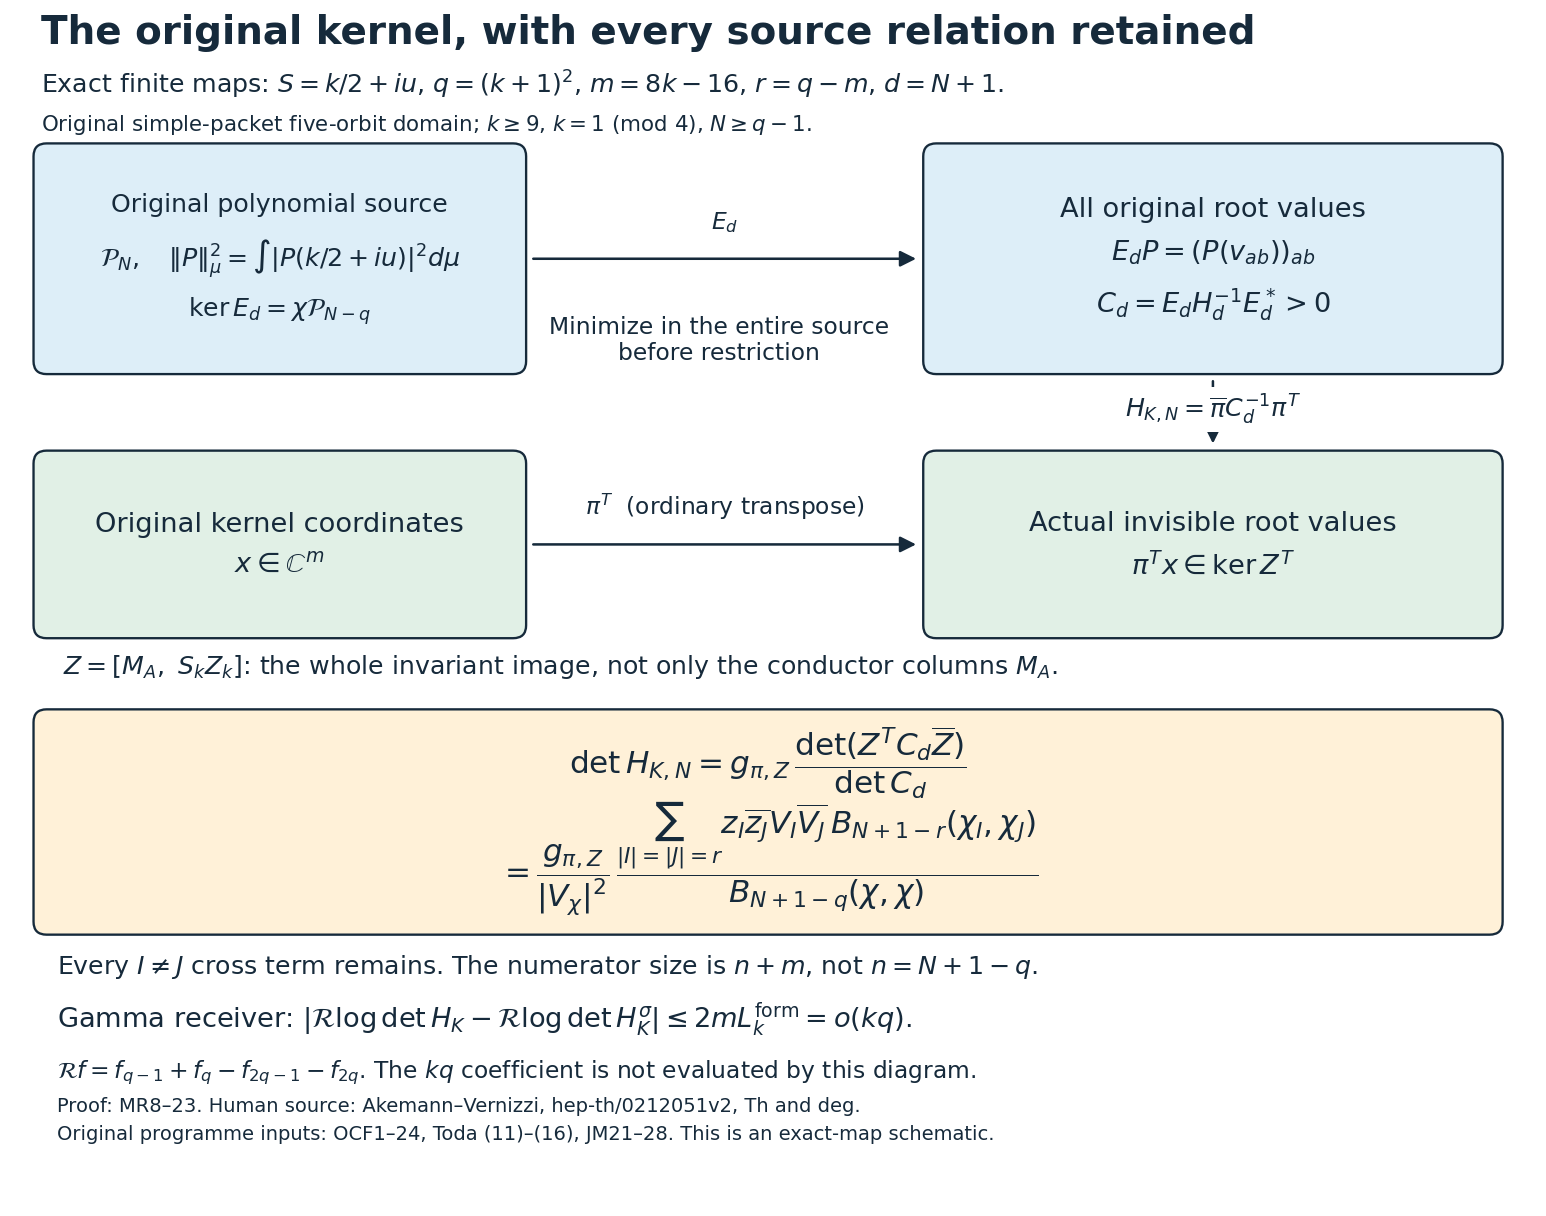
\includegraphics[width=\textwidth,height=.68\textheight,keepaspectratio]{ORIGINAL_KERNEL_MAP.png}\par\par\smallskip\noindent \href{https://github.com/KokunoYumeto/zeta-function-research-reader/blob/5992ad50c0f2a06921f1fcaded7b4e38097c0739/workbenches/splitzero-tandem/continuations/20260920-original-kernel-mixed-determinants/ORIGINAL_KERNEL_MIXED_DETERMINANT.tex\#L36}{Determinant proof MR1--23}; \href{https://github.com/KokunoYumeto/zeta-function-research-reader/blob/5992ad50c0f2a06921f1fcaded7b4e38097c0739/workbenches/splitzero-tandem/continuations/20260920-original-kernel-mixed-determinants/providers/ORIGINAL_CONDUCTOR_STRIP_FRAME.tex\#L27}{Conductor frame OCF1--26}; \href{https://github.com/KokunoYumeto/zeta-function-research-reader/blob/5992ad50c0f2a06921f1fcaded7b4e38097c0739/workbenches/splitzero-tandem/continuations/20260920-original-kernel-mixed-determinants/providers/JOINT_MINIMUM_RECEIVERS.tex\#L286}{Gamma comparison JM21--28}; \href{https://github.com/KokunoYumeto/zeta-function-research-reader/blob/5992ad50c0f2a06921f1fcaded7b4e38097c0739/workbenches/splitzero-tandem/continuations/20260920-original-kernel-mixed-determinants/providers/TODA_VOLUME_CONTROL.tex\#L1}{Original Toda quotient}.\par\smallskip

The diagram records MR1--23, not sampled arithmetic data. Its coefficient
frame contains both the full conductor image and the remaining invariant
directions. The dual map uses an ordinary transpose; the Hilbert Gram uses
adjoints. The positive integral retains every mixed cross term and the
factorial. Its numerator degree is $n+m$, while its denominator degree is
$n$. The preceding Gamma comparison preserves the sought $kq$ coefficient
of the four-cutoff return. The exact finite expression is proved here;
that coefficient has not yet been evaluated.
The human source of the finite characteristic-polynomial identity is
G. Akemann and G. Vernizzi, Nuclear Physics B 660 (2003), 532--556,
arXiv:hep-th/0212051v2, original labels \texttt{Th}, \texttt{Ddef},
\texttt{proof1} and \texttt{deg}. The complete source was read through
its bibliography. The original Toda quotient remains credited to its
preceding programme source, retained in full in the provider directory.
\endgroup
% END COMPLETE ORIGINAL KERNEL MIXED RELATIONS 062

\end{document}
